\documentclass[a4paper,12pt]{report} %use draft mode for rendering tests for formatting but not for the final verson e.g. \documentclass[12pt]

% Figures packages
\usepackage{graphicx}
\usepackage{epstopdf}
\DeclareGraphicsExtensions{.pdf,.gif,.jpg,.eps,.png}
\usepackage{setspace}
\usepackage{float} %needed to force figures in certain place
\usepackage{url}
\usepackage{pdfpages}

% Multi bibliographies
%\usepackage{chapterbib}

% Table packages
\usepackage{booktabs}
\usepackage[flushleft]{threeparttable}
\usepackage{adjustbox}
\usepackage[singlelinecheck=false]{caption}
\usepackage{longtable}
\usepackage{threeparttablex}
\usepackage{rotating}

% %avoid widows and orphans - really important for references
\usepackage[all]{nowidow}

%needed for continuous footnote numbering (requires d/l of chngcntr.sty)
\usepackage{chngcntr}
\counterwithout{footnote}{chapter}

%probably not necessary but may affect output quality if changed
\pdfcompresslevel=1

%set tab to be 0.5 in
\setlength{\parindent}{.5in}

\usepackage{natbib}
\usepackage{chapterbib}

%this makes references be a section style rather than chapter style
%still need to manually add it to TOC in the paper tex file and change the name to REFERNCES
\makeatletter
\renewcommand\bibsection%
{
  \section*{\refname
    \@mkboth{\MakeUppercase{\refname}}{\MakeUppercase{\refname}}}
}
\makeatother
%this removes the ``references'' defined by natbib, and lets you use section names instead,
%which automatically adds it to TOC. Needs the above code to treat refs section as section and not chapter
\renewcommand{\bibsection}{}

%\usepackage{url}
\doublespacing
\usepackage[top=1in, bottom=1in, left=1in, right=1in]{geometry}
\usepackage{amsmath}
\newcommand{\V}[1]{\textup{#1}}
\usepackage{mathtools}
\setcounter{secnumdepth}{5} %this allows use of subsubsections
\setcounter{tocdepth}{5}
\usepackage{graphicx}
%the next three lines are more friendly to foreign (icelandic) fonts
\usepackage[T1]{fontenc}
\usepackage{lmodern} %this is needed with T1
\usepackage[utf8]{inputenc}
\usepackage{listings}

%perform USF style heading formats
%\newcommand{\cchapter}[1]{\chapter[#1]{\centering #1}}
\usepackage{titlesec}

%needed to not center abstact vertically on center of page and bring it to top instead
\usepackage{etoolbox}

%TOC stuff
\usepackage{alltt}
%TOC INDENTATION
\usepackage[titles]{tocloft}

%next three blocks control heading indents	
\titlespacing{\chapter}{0em}{.68in}{2em}
\titleformat{\chapter}
  {\normalfont\bfseries\centering}{\thechapter}{1em}{}

\titlespacing{\section}{0em}{1em}{0em}
\titleformat{\section}
  {\normalfont\bfseries\raggedright}{\thesection}{1em}{}

\titlespacing{\subsection}{.5in}{1em}{0em}
\titleformat{\subsection}
  {\normalfont\bfseries}{\thesubsection }{1em}{}
  
%format the table of contents
\makeatletter
\def\tableofcontents{%
 \newpage
\vspace*{.82in}
 \centerline{\bf Table of Contents}
 \vspace*{2em}
 \@mkboth{CONTENTS}{CONTENTS}
 \@starttoc{toc}
}
\makeatother

%format the list of tables 
\makeatletter
\def\listoftables{%
	\newpage
	\vspace*{.80in}
	\centerline{\bf List of Tables}
	\vspace*{2em}
	\@mkboth{CONTENTS}{CONTENTS}
	\@starttoc{lot}
}
\makeatother

%format the list of figures 
\makeatletter
\def\listoffigures{%
 \newpage
\vspace*{.80in}
 \centerline{\bf List of Figures}
 \vspace*{2em}
 \@mkboth{CONTENTS}{CONTENTS}
 \@starttoc{lof}
}
\makeatother

%get rid of leader dots in TOC and LOF
\renewcommand{\cftdot}{}

%this part of the code ensures that there is a period after the number, e.g. 1. CHAPTERNAME
\makeatletter
\renewcommand{\@makechapterhead}[1]{%
{ \vspace*{.5in} }
{\setlength{\parindent}{0pt} \center \normalfont
\bfseries\thechapter.\ #1
\par\nobreak\vspace*{\baselineskip}}}
\makeatother


%figure stuff - leave as is (may be important if figures are inside the text rather htan at the end of the chapters)
\widowpenalty=10000
\clubpenalty=10000


%this controls the TOC indentation
\renewcommand{\cftsecindent}{.5in}
%\renewcommand{\cftsecnumwidth}{1.9 em}
\renewcommand{\cftsubsecindent}{1in}
%\renewcommand{\cftsubsecnumwidth}{2.8 em}	
\renewcommand{\cfttabfont}{Table }
\renewcommand{\cftfigfont}{Figure }
%these should change the table of contents main headings to not be bold
\renewcommand\cftchapfont{\mdseries}
\renewcommand\cftchappagefont{\mdseries}


%define page nums to be .25" below text
\setlength{\footskip}{0.25in}

%this controls vertical spacing, NECESSARY FOR DOUBLE SPACING BETWEEN TITLES
\setlength{\cftbeforetabskip}{1em}

%this should set indent level for Figure X....(0 inches so that its at left margin)
\setlength{\cftfigindent}{0in}
%note that the Figure X and the rest of the text are tied, so the above value should be 0

%this controls vertical spacing, NECESSARY FOR DOUBLE SPACING BETWEEN TITLES
\setlength{\cftbeforefigskip}{1em}
%this controls distance between figure X: ____ NAME
% \setlength{\cftfignumwidth}{.5in}

%this is needed to keep proper indentation in two-line figure label text
%ALL OF THESE ARE NECESSARY
\renewcommand{\cftfigfont}{}
\renewcommand{\cftfigpresnum}{Figure }             	
\renewcommand{\cftfigaftersnum}{}  
\renewcommand{\cftfigpagefont}{}                      
\renewcommand{\cftfignumwidth}{1in}

%this is needed to keep proper indentation in two-line table label text
%ALL OF THESE ARE NECESSARY
\renewcommand{\cfttabfont}{}
\renewcommand{\cfttabpresnum}{Table }             	
\renewcommand{\cfttabaftersnum}{}  
\renewcommand{\cfttabpagefont}{}                      
\renewcommand{\cfttabnumwidth}{1in}

%this will redefine the width of the pagenumbering on the TOC/LOF (3 font units (e.g. for pages containing three characters like 113)
\makeatletter\renewcommand{\@pnumwidth}{3em}\makeatother

%this lets the chapter names and figure captions end at 0.5 in from the right per usf rules
\makeatletter\renewcommand{\@tocrmarg}{0.5in}\makeatother

%remove extra space in List of Figures between header and the figure list
\addtocontents{lof}{\protect\renewcommand*\protect\addvspace[1]{}}
%MUST DO SAME FOR TOC, NOT YET DONE????????

%control spacing inside LOF
%???????
% \renewcommand{\cftfigafterpnum}{1.25in}
%
%\makeatletter
%\def\@makeschapterhead#1{%
%  \vspace*{.6in}% space before the title
%  {\center
%    \normalfont
% \bfseries  #1\par\nobreak
%    \vskip 12\p@ % space after the title
%  }}
%\makeatother

%this is an OVERFULL eliminator - if black rectangle appears in text, this gets rid of it DO NOT REMOVE THIS 
\setlength{\emergencystretch}{2em}

%needed to not center abstact vertically on center of page and bring it to top instead
% \usepackage{etoolbox}
% \patchcmd{\abstract}{\null\vfil}{}{}{}


\begin{document}

%TITLE PAGE FILE GOES HERE
\begin{titlepage}
\begin{center}
\singlespacing
% { \vspace*{\baselineskip} }
{ \vspace*{\baselineskip} }
{ \vspace*{\baselineskip} }
{ \vspace*{\baselineskip} }
{ \vspace*{\baselineskip} }
Glaciological Applications of Terrestrial Radar Interferometry\\
{ \vspace*{\baselineskip} }
{ \vspace*{\baselineskip} }
{ \vspace*{\baselineskip} }
by\\
{ \vspace*{\baselineskip} }
{ \vspace*{\baselineskip} }
{ \vspace*{\baselineskip} }
Denis Voytenko\\
{ \vspace*{\baselineskip} }
{ \vspace*{\baselineskip} }
{ \vspace*{\baselineskip} }
{ \vspace*{\baselineskip} }
A dissertation submitted in partial fulfillment\\
of the requirements for the degree of\\
Doctor of Philosophy\\
School of Geosciences\\
College of Arts and Sciences\\
University of South Florida\\
{ \vspace*{\baselineskip} }
{ \vspace*{\baselineskip} }
{ \vspace*{\baselineskip} }
Major Professor: Timothy H. Dixon, Ph.D.\\
Rocco Malservisi, Ph.D.\\
Kenneth C. Jezek, Ph.D.\\
H.L. Vacher, Ph.D.\\
Charles L. Werner, Ph.D.\\
{ \vspace*{\baselineskip} }
{ \vspace*{\baselineskip} }
Date of Approval:\\
March 9, 2015\\
{ \vspace*{\baselineskip} }
{ \vspace*{\baselineskip} }
{ \vspace*{\baselineskip} }
Keywords: ground-based interferometry, iceberg tracking, remote sensing, ice-ocean interactions\\
{ \vspace*{\baselineskip} }
%the hspace is needed to put space beween the C and the year, which is not done by default
Copyright \copyright\hspace{1mm}2015, Denis Voytenko\\
\end{center}
\end{titlepage}

%ACKNOWLEDGE PAGE FILE GOES HERE
%\chapter*{Dedication}
\thispagestyle{empty}
\doublespacing
\begin{center}
I dedicate this dissertation to God.

And He said to me, "My grace is sufficient for you, for My strength is made perfect in weakness." (2 CORINTHIANS 12:9)
\end{center}
\chapter*{Acknowledgements}
\thispagestyle{empty}
\doublespacing
This dissertation would not have been possible without the help of so many individuals.  First and foremost, I cannot thank my advisor, Timothy H. Dixon, enough for guiding and supporting me over the years.  I’m grateful to have such an inspiring and encouraging advisor and I truly admire his enthusiasm for sciences. I would like to thank my committee.  To Rocco Malservisi, thank you for helping me with GPS processing and numerical modeling.  To Don Chamber, thank you for your vital contribution to Chapter 4.  To Ping Wang, thank you for your support throughout the stages of this dissertation.
Thanks to my scientific collaborators Shimon Wdwinski, Paul G. Myers, Jennifer Bonin, M.R. van den Broeke, Weon Shik Han, Wenliang Zhao, Falk Amelung who contributed greatly to this dissertation.  To Denis Voydenko, thank you for helping me to solve many technical issues.  To Laura Connor, thank you for maintaining the computer systems at the geodesy lab.  To every member in the geodesy lab, thank you for creating such a positive work environment.
I would like to thank my friends.  To Amanda Piggot, thank you for helping me to improve my English and driving me to school the first semester when I was in the US.  To Meng Wang and Wen Zhao, thank you for taking me in your place and driving me to school when I visited Tampa.
Last, but certainty not least, I would like to thank my families. To my parents and my grandma, thank you for your endless love and support.   To my beloved husband Peng Li, thank you for being so loving and making me complete.  

\pagenumbering{roman}
\begin{singlespace}
%\vspace*{1in}

\tableofcontents

\end{singlespace}


%not sure what this does
\renewcommand{\cftsecleader}{\cftdotfill{\cftdotsep}}



%LOT needs to have singlespacing between lines continued onto a second line. The extra spacing between each figure is forced elsewhere in the preamble.
\begin{singlespace}
\cleardoublepage
\addcontentsline{toc}{chapter}{List of Tables}
\listoftables
\end{singlespace}

%LOF needs to have singlespacing between lines continued onto a second line. The extra spacing between each figure is forced elsewhere in the preamble.
\begin{singlespace}
\cleardoublepage % Start a new page for the list of figures. Make it right handed for two-sided documents.
\addcontentsline{toc}{chapter}{List of Figures} % add to table of contents.
\listoffigures % generate the list of figures
\end{singlespace}

%\patchcmd{\abstract}{\null\vfil}{\vspace*{37pt}}{}{}
\patchcmd{\abstract}{\null\vfil}{\vspace*{30pt}}{}{}
\begin{abstract}
\thispagestyle{plain}
Space geodesy plays an important role in earth observation. This dissertation presents three applications of satellite geodesy in environmental and climate change. Three satellite geodesy techniques are used: high-precision Global Positioning System (GPS), the Gravity Recovery and Climate Experiment (GRACE) and Interferometric Synthetic Aperture Radar (InSAR).  
In the first study, I use coastal uplift observed by GPS to study the annual changes in mass loss of the Greenland ice sheet.  The data show both spatial and temporal variations of coastal ice mass loss and suggest that a combination of warm atmospheric and oceanic condition drove these variations.  
In the second study, I use GRACE monthly gravity change estimates to constrain recent freshwater flux from Greenland.  The data show that Arctic freshwater flux started to increase rapidly in the mid-late 1990s, coincident with a decrease in the formation of dense Labrador Sea Water, a key component of the deep southward return flow od the Atlantic Meridional Overturning Circulation (AMOC). Recent freshening of the polar oceans may be reducing formation of Labrador Sea Water and hence may be weakening the AMOC.  
In the third study, I use InSAR to monitor ground deformation caused by CO$_{2}$ injection at an enhanced oil recovery site in west Texas.  Carbon capture and storage can reduce CO$_{2}$ emitted from power plants, and is a promising way to mitigate anthropogenic warming.  From 2007 to 2011, $\sim$24 million tons of CO$_{2}$ were sequestered in this field, causing up to 10 MPa pressure buildup in a reservoir at depth, and surface uplift up to 10 cm.  This study suggests that surface displacement observed by InSAR is a cost-effective way to estimate reservoir pressure change and monitor the fate of injected fluids at waste disposal and CO$_{2}$ injection sites.  
\setcounter{page}{8} %NEEED TO MANUALLY SET PAGE HERE
\addcontentsline{toc}{chapter}{Abstract}
\end{abstract}

\pagenumbering{arabic}
%use the intro paragraph here, must define chapter and label in the other tex file
%need to remove all of the journal-specific formatting stuff from the tex files in the separate chapter files
\chapter{Introduction}
\section{Overview}
Satellite geodesy is the measurement of the size and shape of the earth as well as its gravity field by means of artificial satellites.  Satellite geodesy is a powerful tool to monitor time variations in the Earth related to plate tectonics, post-glacial rebounds, ocean circulation, ground water extraction, and a host of other natural and anthropogenic processes.  This dissertation focuses on the application of satellite geodesy to studies of environmental and global change.  Data from three techniques are used: high precision Global Positioning System (GPS), Interferometric Synthetic Aperture Radar (InSAR) and the Gravity Recovery and Climate Experiment (GRACE).  

The dissertation has six chapters. Chapter One (this chapter) is an introduction and summary of the work.  Chapter two describes the essentials of three satellite geodesy techniques.  The next three chapters (Chapter Three, Four and Five) are each based on a published, open literature paper.  

Chapter Three focuses on using coastal vertical displacement observed by high precision GPS to study recent mass loss of the Greenland ice sheet.  High precision GPS has been used to study a number of Earth processes, including plate motion, fault-related crustal deformation, and coastal subsidence.  Many of these applications involve looking at secular (long-term) rates of surface deformation, where the displacement rate can be assumed constant over the measurement period, typically several years or longer.  In a number of Earth processes, however, it is also useful to consider short-term fluctuations.  Many of these applications involve changes in Earth's fluid envelope, for example annual loading and unloading of the crust associated with the hydrologic cycle.  Accelerating uplift of the coastal regions of Greenland, where most of the current mass loss is concentrated \cite[e.g.,][]{zwally2005intro,thomas2006intro,luthcke2006intro,rignot2006intro,wouters2008intro}, is well recorded by a network of GPS stations emplaced on the rocky margins \cite[]{bevis2012intro}.  The previous study of \citet{jiang2010intro} focused on decadal scale trends and demonstrated that decadal time series of the vertical position component were well fit by a simple model of constant acceleration.  \citet{jiang2010intro} assumed constant amplitude of annual uplift each year, a common assumption in GPS time series analysis. However, the data show significant annual variation.  More recent measurements suggest that accelerating melting of Greenland ice sheet is continuing, with some melting seasons (for example 2010, 2012) experiencing significant ice mass loss \cite[]{bevis2012intro,nghiem2012intro}.  Thus, the short-term annual variation of coastal uplift measured by GPS can be useful in studying variable and accelerating ice mass loss.

One important aspect of the current retreat phase in Greenland is the role of climate forcing on melting coastal areas of Greenland.  In Greenland, ice mass change is regulated by two climate factors, atmospheric forcing \cite[]{zwally2002intro,hall2008intro} and oceanic forcing \cite[]{van2008intro,holland2008intro,hanna2009intro,straneo2010intro,straneo2012intro,straneo2013intro,seale2011intro}.  Atmospheric forcing can affect surface mass balance (SMB) by changing either or both the snow accumulation rate and the ablation rate. Also, melt water can influence the basal sliding rate. Oceanic forcing can increase submarine melting of marine-terminating outlet glaciers, resulting in rapid changes in calving rate, and inducing dynamic changes upstream, including glacier acceleration and thinning \cite[]{straneo2013intro}.  GRACE satellite data documents mass loss in Greenland over the last decade, and for West Greenland, clearly shows that loss is concentrated along the coast \cite[e.g.,][]{wouters2008intro}.  Unfortunately these data lack the spatial resolution to investigate melting at the scale of individual drainage basins.  However, coastal uplift as measured by GPS is sensitive to ice loss at this scale, which allows assessment of the influence of local climate conditions on melting.   In my dissertation, both short-term and long-term surface deformation processes measured by GPS is utilized to understand the climatic forcing on mass loss. What are the main driving forces for recent accelerated mass loss of Greenland Ice Sheet?  What is the relative contribution of oceanic versus atmospheric forcing on coastal melting?  Those questions will be discussed in my dissertation by using GPS data combined with other oceanographic and meteorological data.

Chapter Four uses GRACE data to estimate the recent freshwater flux from Greenland and investigates its impact on the Atlantic Meridional Overturning Circulation (AMOC).  The AMOC is a major mode of ocean thermo-haline circulation.  It is driven by density differences in the Atlantic Ocean, and is a key component of the global climate system.  Both theoretical and numerical studies show that the AMOC is sensitive to freshwater balance because of the strong influence on sea water density \cite[]{stommel1961intro,rooth1982intro,rahmstorf1995intro,stouffer2006intro}.  Past abrupt climate changes have been linked with changes in the AMOC in response to changes in the freshwater budget \cite[]{manabe1993intro,manabe1995intro,clark2002intro}.  Recent anthropogenic warming and accelerated melting of the Greenland ice sheet is leading to a general freshening of the North Atlantic, raising concerns that the AMOC may soon be disrupted.  

In this dissertation, I estimate Arctic freshwater flux from three sources that are undergoing rapid increases and can be estimated from remote observations: the Greenland ice sheet, CAA glaciers and Arctic sea ice.  Among these, freshwater flux from Greenland is the largest component, and estimated with GRACE data and RACMO2.3 model \cite[]{ettema2009intro,noel2015intro}.  The pattern of coastal currents around Greenland tends to focus coastal waters towards the Labrador Sea, an important ``incubator'' for dense, North Atlantic Deep Water (NADW).  Southward return flow of NADW is an important component of the AMOC, hence any disruption of density balance in the Labrador Sea may be a leading indicator of changes to the AMOC.  In this dissertation, I compare freshwater flux estimates to properties of Labrador Sea Water and suggest that increased freshwater flux here is starting to impact the AMOC.  

Chapter Five focuses on using surface deformation observed by InSAR to study reservoir pressure change caused by fluid injection and production at an enhanced oil recovery field.  Similar to GPS, InSAR has been used to study a number of Earth processes.  Particularly, it has been used to monitor ground subsidence associated with oil and gas extraction \cite[]{tomas2005intro}.  As oil reservoirs have been drawn down in the last few decades, producers have increasingly applied enhanced oil recovery (EOR) techniques to increase the amount of oil that can be extracted from a given oil field.  This usually involves pumping of CO$_{2}$ or saline water into the reservoir, and raising the reservoir pressure.  Similar techniques are used in ``fracking'' (hydraulic fracturing) to stimulate natural gas production, and later, to get rid of water.  In some regions, there is concern that rapid pumping of water fluids into deep reservoirs can stimulate induced seismicity \cite[e.g.,][]{keranen2013intro,mcgarr2015intro}.  Here, there is a need for research into the rock mechanical and fluid mechanical processes involved in such fluid pumping.  There is also interest in pumping CO$_{2}$ from industrial plants into deep geological formations for large-scale Carbon Capture and Storage (CSS), thereby reducing CO$_{2}$ emissions to the atmosphere.  Research is underway to study the geomechanical impact of CCS, including microseismicity, fault reactivation, fracturing and ground deformation \cite[e.g.,][]{streit2004intro,zhou2010intro,mazzoldi2012intro,rinaldi2013intro,vasco2010intro}.  Here, ground deformation associated with fluid injection and production is studied to better understand the links between surface deformation and pressure changes at depth.  A numerical model incorporating rock and fluid properties is constructed to relate surface deformation to pressure changes at depth.  My method offers an inexpensive way to monitor deep reservoir pressure change based on low cost commercial satellite imagery.  

Chapter Six summarizes the main conclusions from the previous chapters, and makes suggestions for future research.  

\section{References}
\bibliographystyle{apalike}  
\bibliography{intro_ref}
\chapter{Technical Background}
\section{Global Positioning System}
The Global Positioning System (GPS) has developed by the U.S Department of Defense (DoD) to provide civilian and military users with worldwide positioning, navigation and timing services.  Here, a brief introduction about principles of GPS and errors sources of GPS position measurement is presented.  For detailed studies, the reader is referred to special literatures, \citet[e.g.,][]{dixon1991chpt2,mao1999noise,hofmann2001gps}
  
\subsection{Struture}
The GPS system consists of three segments: the space segment, the control segment, and the user segment.  The space segment consists of the GPS satellites that transmit radio signals to users.  The nominal GPS constellation consists 24 satellites that are equally spaced in 6 orbital planes with 4 satellites in each plane.  Orbital planes are 60 degree separated and inclined at about 55 degree respect to the equatorial plane.  Each satellite flies in medium Earth orbit at an altitude of about 20200 km and circles the Earth twice a day.  This constellation ensures users can view at least 4 satellites from any point on the earth. The control segment on the ground consists of a system of facilities that receive signals from the satellites, perform analysis to compute satellite orbital data (ephemerides) and clock corrections, and send ephemerides back to each satellite.  The user segment consists of the GPS receivers that receive the signals from the GPS satellite and convert them into three-dimensional position and time. 

\subsection{GPS signal}
Each GPS satellite transmit microwave signal on two carrier frequencies: L1 (1575.42 MHz) and L2 (1227.60 MHz).  Two pseudorandom noise (PRN) codes and navigation message are modulated into the carrier frequencies.  The Coarse/Acquisition (C/A) code is modulated into the L1 carrier. The Precision (P) code is modulated into the L1 and L2 carriers.  The P-code is encrypted into Y-code in the Anti-Spoofing (AS) mode, which denies unauthorized users to use it.  Note that as a major focus of the GPS modernization program, three new civil (L1C, L2C, L5) signals and a new military (M) signal are added to the L1 and L2 carriers. 

\subsection{GPS basic observations}
To determine three-dimensional position of a user, the GPS receiver should compute the range to at least four satellites combing with satellites positions at time of transmitting signals.  However, due to synchronism problem between satellite clock and receiver clock and other factors, the GPS receiver can only provide pseudorange measurements rather than the true geometry range.  GPS receivers are capable to provide two types of pseudorange observations: code pseudorange and carrier phase pseudorange observations.  The code pseudorange is obtained by multiplying the speed of light by the travelling time, where the travelling time is determined by correlating the received code (C/A or P(Y)) from the satellite with the replicas generated by the receiver.  The carrier phase pseudorange is obtained by multiplying the wavelength by difference between carrier phase from the satellite and the carrier phase generated by the receiver.  Carrier phase pseudorange is about two orders of magnitude precise than the code pseudorange, but the carrier phase observation is ambiguous by an integer number of cycles \cite[]{remondi1985global}.  In order to achieve millimeter-precision, the ambiguity problem is needed to be fixed.  Carrier phase ambiguity resolution has been studied by \citet{lichten1987strategies}, \citet{blewitt1989chpt2,blewitt2008chpt2} and \citet{bertiger2010chpt2}. 
 
\subsection{GPS error sources}
There are many sources of error that will contaminate the position measurements. Major GPS error sources are briefly discussed in below.

(i) Satellite clock and orbit errors

GPS satellite clock time should be synchronous with GPS time (the time scale used by the GPS system).  Error in the satellite clock has a major impact on the computed code pseudorange.  Satellite orbits error is the discrepancies between the predicted position of each satellite and the true satellite position, causing error in the computed position.  In this dissertation, we use the precise final orbits and adjusted clock products provided by the Jet Propulsion Laboratory to mitigate satellite clock and orbit errors.  Another source of precise satellite orbits and adjusted clock products is the International GNSS Service (IGS).

(ii) Atmospheric effects  

The GPS signals encounter both inonspheric refraction and tropospheric refraction when propagating through the atmosphere, causing propagation delay.  The ionospheric delay is frequency dependent and can be corrected by using dual frequency (L1/L2).  The tropospheric effect can be reduced by using an elevation mask to avoid receiving signals from satellites lower than a certain elevation.  The tropospheric delay must be modeled.  The tropospheric model consists of mean tropospheric parameters or measurements data (temperature, air pressure, water vapor) and a mapping function \cite[]{niell1996chpt2,bohm2006chpt2,boehm2006chpt2}.  

(iii) Multipath effects

Multipath effects means receiver antenna gets direct signal through straight-line path and reflected signals through multiple paths. Multipath effects on code observation are much larger than on the carrier-phase observation.  Due to the randomness, the multipath effects cannot be modeled.  But it can be reduced with relatively long time observations.  In our processing routine, we estimate observations every 24 hours to minimize the multipath error \cite[]{sella2002chpt2}. 

(iv) Antenna phase center offset and variation 

The electrical antenna phase center (APC) is the point in space where radio signal is received.  However, the position of APC varies depending on the intensity and direction of incoming signal.  Thus, antenna phase center variation (PCV) is defined as the difference between the APC of each measurement and the mean position of the electrical antenna phase center (MPC).   The antenna phase center offset (PCO) is defined as the difference between MPC and antenna reference point (ARP) given by the manufacture.  An absolute phase center correction model estimated by \citet{schmid2007intro} can be use to calibrate both GPS satellite and receiver antennas. 

Note that here only the major error sources are discussed.  Other factors such as receiver clock error, monument movement and software accuracy also cause errors in GPS position results.  Last but not least, deformations due to ocean tidal, earth tidal and atmospheric loading need to be modeled and removed so that the geophysical process of interest (e.g., ice mass loss) can be isolated from other geophysical processes.  
   
\section{Interferometric Synthetic Aperture Radar}

\section{Gravity Recovery and Climate Experiment}

\section{References}
\bibliographystyle{apalike}  
\bibliography{chpt2_ref}
\chapter[Annual Variation of Coastal Uplift in Greenland as an Indicator of Variable and Accelerating Ice Mass Loss]{Annual Variation of Coastal Uplift in Greenland as an Indicator of Variable and Accelerating Ice Mass Loss \footnote{This chapter has been reprinted from Geochemistry Geophysics Geosystems with permission as: Yang, Q., Wdowinski S., Dixon, T. H., (2013), Annual variation of coastal uplift in Greenland as an indicator of variable and accelerating ice mass loss, Geochem. Geophys. Geosyst., 14, 1569–1589, doi:10.1002/ggge.20089.}}

\section{Abstract} 
Seasonal melting of the coastal part of the Greenland ice sheet is investigated using GPS vertical displacement data from coastal stations, combined with data on atmospheric and ocean temperatures.
Using a high pass filter and cubic spline models, we estimate five variables describing seasonal uplift, a proxy for proximal mass loss, including duration of the melt season and the amount of summer uplift. Our analysis shows both temporal and spatial variations of uplift. Southern coastal Greenland experienced
anomalously large uplift in summer 2010, implying significant melting that year. However, the northwest coast did not experience significant change in uplift at that time. Our data suggest that a combination of warm summer air temperature and warm sub-surface ocean water temperature drove the large mass losses in 2010. Using the uplift pattern of 2008–2010, and comparing to atmospheric data and ocean water temperature data, we show that warm Irminger Water (IW) exerted significant influence on coastal melting in southeastern, southern and southwestern Greenland, reaching about 69 \textordmasculine N in 2010. North of this, IW did not exert significant influence, in effect defining the northward limit of the sub-polar gyre for that year. Thus, short-term variability in the coastal GPS uplift signal can be used to infer an oceanographic parameter that has a critical influence on Greenland ice sheet health.

\section{Introduction}
Significant mass loss of the Greenland ice sheet
has been revealed in the last decade by the GRACE
gravity mission \cite[]{velicogna2006acceleration,velicogna2009increasing,chen2006satellite,luthcke2006recent,van2009partitioning,jacob2012recent}, satellite altimetry \cite[]{krabill2004greenland,zwally2005mass,thomas2006progressive},mass accumulation/loss estimates \cite[]{hanna2005runoff,rignot2006changes,rignot2008mass}, and GPS observations of coastal uplift \cite[]{jiang2010accelerating,khan2010spread,bevis2012bedrock}. Recent studies detect considerable spatial
and temporal variability of ice sheet mass change: prior to the 2010 melt season, mass loss appeared to be accelerating along the northwest coast, but slowing down in southeast Greenland since 2007 \cite[]{khan2010spread,murray2010ocean,chen2011interannual}. Subsequently, \cite{box2010greenland} reported
anomalously high air temperatures and melting in summer 2010 for much of coastal Greenland. 

Coastal uplift is a useful proxy for coastal mass loss and perhaps overall Greenland ice mass balance. Previous studies have demonstrated that accumulation and loss in the interior of Greenland are in approximate balance, while recent net losses are focused in marginal coastal areas \cite[e.g.,][]{zwally2005mass,thomas2006progressive,luthcke2006recent,rignot2006changes,wouters2008grace}. These coastal losses result in significant coastal uplift, reflecting the short-term, elastic response of the crust to mass unloading, and are readily measured by high precision GPS \cite[]{jiang2010accelerating,khan2010spread,bevis2012bedrock}. Our previous study focused on decadal scale trends
and demonstrated that decadal time series of the vertical position component were surprisingly well fit by a simple model of constant acceleration, with values for some Greenland stations, up to the end of the 2008 melt season, approaching 1mm yr$^{-2}$ \cite[]{jiang2010accelerating}. More recent measurements suggest that this trend of accelerating melting and uplift is continuing, at least at some locations, with the 2010 melt season recording the largest uplift since measurements began at many localities \cite[]{bevis2012bedrock}.

\cite{jiang2010accelerating} also suggested that there was useful information in the annual variation of coastal
uplift. In Greenland, ice mass change is regulated by two climate factors, atmospheric forcing \cite[]{zwally2002surface,hall2008greenland} and oceanic forcing \cite[]{van2008large,holland2008acceleration,hanna2009hydrologic,straneo2010rapid,straneo2012characteristics,seale2011ocean}. Atmospheric forcing can affect surface mass balance (SMB) by changing either or both the snow accumulation rate and the ablation rate. Also, melt water can influence the basal sliding rate. Oceanic forcing can increase submarine melting of marine-terminating outlet glaciers, resulting in rapid changes in calving rate, and inducing dynamic changes upstream, including glacier acceleration and thinning. For both atmospheric and oceanic forcing, most melting occurs during the warm summer months and at low elevations near the coast. Nevertheless, it may be possible to use the
summer uplift signal to separate the various effects and elucidate controls on mass loss. In this paper, we focus on seasonal uplift patterns in GPS data by using a high pass filter and cubic spline fit to the vertical position time series. We investigate regional and temporal changes in annual uplift and, by implication, coastal melting, and attempt
to separate the relative roles of oceanic versus atmospheric forcing.   
 
\section{Methods}

\subsection{GPS Data and Processing}
We analyzed all publicly available GPS data
up to May 2011. Data from 18 continuous or
semicontinuous GPS sites in the coastal region of
Greenland are now available with at least 3 years of
data, through the establishment of a remarkable
network of reliable, high precision instruments \cite[]{bevis2012bedrock} (Figure \ref{fig:fig1}). We use the
GIPSY-OASIS 5.0 software \cite[]{zumberge1997precise} to process these data. Orbit parameters and
clock products are provided by Jet Propulsion
Laboratory (ftp://sideshow.jpl.nasa.gov/). We use
the Global Mapping Function \cite[]{bohm2006global}
to relate the atmospheric wet delay to elevation
angle. An ocean tidal loading correction is applied
to all sites by using model FES2004 \cite[]{letellier2005etude}. We first generate daily precise point position
solutions for each station. We then adopt the
Ambizap algorithm \cite[]{blewitt2008fixed} to solve integer
ambiguities for each station. The final ambiguity fixed
daily solutions are then aligned to the IGS05
reference frame \cite[]{altamimi2007itrf2005}. Errors
associated with GPS reference frame instability are
probably negligible for the short-term (2008–2010)
comparisons that are the main focus of our study,
although they could affect longer-term (decadal)
time series. 

To isolate the effect of ice load variation from seasonal atmosphere loading, we apply an air pressure loading correction.  We subtract precomputed Atmospheric Loading Displacements (http://gemini.gsfc.nasa.gov/aplo/) \cite[]{petrov2004study}from the GPS vertical displacement time series.  Details of this precedure are described in the supporting information section.  

We also considered the possibility of local snow loading as a source of annual uplift variability. Calculations suggest that the deformation caused by local snow load is less than 1mm at most of our study sites (supporting information), so we have ignored this effect.

\subsection{Seasonal Uplift Analysis}
\cite{jiang2010accelerating} assumed constant amplitude of annual uplift each year, a common assumption in GPS time series analysis. However, the data show significant annual variation, and it is this variation that we seek to quantify. Variable amplitude in the seasonal signal has been addressed in several ways \cite[]{murray2005spatiotemporal,davis2006subcontinental,bennett2008instantaneous,davis2012seasonal}. In this paper, we first use a high pass filter to isolate the seasonal signal by removing the secular component from the GPS time series. We then fit the residual GPS time series with a smoothing cubic spline. Based on the spline model estimate (red solid line in Figure \ref{fig:fig2}), we derive five variables that relate to mass loss: the timing (start and end time) and duration of summer melt season, the total amount of seasonal uplift (which relates to the total mass loss, including surface and sub-surface melting, runoff, calving, and dynamic thinning) for the local basin, and the rate of summer uplift (Figure \ref{fig:fig2}). We chose a cubic spline model because it is straightforward to apply and can identify the minima and maxima for each year without any assumptions concerning specific periodicity, which may vary from year to year. 

A key parameter in the cubic spline model is the smoothing, S. As the value of S increases, misfit decreases, but the “roughness” (complexity) of the model increases; at some point, more than one maxima and minima per year can result, which is generally unrealistic. Thus, there is a trade-off between goodness of fit and smoothing. A sensitivity
study using various values of S allows us to define an optimum value by requiring a single crest and a single trough per year. The optimum smoothing parameter differs somewhat for each site because of variations in data quality and length of time series. We chose a compromise value ($S$=0.91) and applied it to all sites to ensure that relative
variations in estimated parameters can be compared across all the time series and regions in a consistent way. This value generates single minima and single maxima per year for 16 out of 18 sites. For sites THU3 and QAQ1, the analysis yields double peaks in 2007 and 2008, respectively, although one is smaller than the other. For these two sites, we remove the smaller crest and trough, using the larger one to estimate the five parameters of interest. These sites are marked with an asterisk in Table \ref{tab:chpt3_table1}. Note that the seasonal uplift estimated in this way is somewhat conservative, especially for years with significantly different uplift compared to earlier years. This reflects the fact that our technique tends to damps extreme excursions, with the effect increasing as the degree of smoothing increases. All time series and their spline model fits are shown in the supporting information.

Uncertainties for the parameter estimates are determined with a Monte Carlo approach. We report the mean value of a large number of estimates as the best estimate, with uncertainty defined at the one-sigma confidence level based on the bounds containing 68\% of the estimated values. Details of this procedure are described in the supporting information section.

\subsection{Surface Air Temperature Data and Analysis}
We obtained daily surface air temperature data from 11 meteorological stations in coastal Greenland provided by the Danish Meteorological Institute \cite[]{carstensen2011weather}. All the stations are synoptic and observe surface air temperature and other weather parameters at 3 h intervals. We select the meteorological sites that have a similar time span to the GPS data and are closest to the GPS site of interest (Figure \ref{fig:fig1}). Information describing these meteorological stations and respective nearby GPS stations are listed in Table \ref{tab:SI_chpt3_table2}. The time span for available meteorological records near KULU and KELY is 2000–2010; for QAQ1 and THU3, it is 2003 – 2010; for other GPS stations, it is 2008–2010. In order to compare air temperature with annual uplift variability, we calculate the Annual Mean Surface Air Temperature (AMSAT) and Cumulative Annual Positive Degree Days (CAPDD) per year for each meteorological station. CAPDD may be a better indicator of seasonal, atmospheric-forced melting than AMSAT; on the other hand, AMSAT
is a simple indicator of overall climate warming. It is also useful to compare AMSAT with annual mean ocean temperature, discussed later.

\subsection{SMB}
SMB is the difference between net snow accumulation and net runoff of surface meltwater. Since coastal uplift recorded by GPS is caused by both nearby SMB changes and ice dynamic changes (mainly calving and associated thinning),
comparison of the GPS results to SMB changes provides an alternate way to assess atmospheric versus oceanic forcing. We use SMB derived from Regional Atmospheric Climate Model v.2 (RACMO2) \cite[]{ettema2009higher,ettema2010climateA,ettema2010climateB,kuipers2011new,van2012sensitivity} and calculate SMB in the summertime (June to August) in each year during 2000–2010.

\subsection{Sub-surface Ocean Temperature Data and Analysis}
Sub-surface water temperature is obtained from the Hadley Center EN3 model output (http://www.metoffice.gov.uk/hadobs/en3/). The EN3 model consists of two products: (1) in-situ sub-surface ocean temperature and salinity profiles with data quality information; and (2) objective analyses using optimal interpolation of the in-situ data profiles with a quality control system \cite[]{ingleby2007quality}. In this paper, we use the objective analyses product, which contains monthly temperature estimates from 1950 to the present with a spatial resolution of 1 $\textordmasculine$ $\times$ 1 $\textordmasculine$ (about 111 km (N-S) by 38 km (E-W) at 70 $\textordmasculine$ north, neat central Greenland) and 42 depth intervals (5m to 5350 m). Due to the presence of a broad continental shelf, water depth along most of Greenland’s coast is limited, which in turn limits the influence of deep water. We looked at data in the EN3 model from 5m to 447m depth (depth levels 1 to 22), selecting 14 “voxels” (model volume elements) that are close to our GPS stations (Figure \ref{fig:fig1}). To compare sub-surface water temperature with annual uplift and atmospheric mean temperature, we calculate the Annual Mean Sub-Surface Water Temperature (AMSSWT) averaged over this upper 442m of ocean depth range. The deeper parts of this water volume will not necessarily interact with all outlet glaciers due to topographic barriers near a given fjord entrance (usually endmoraines from the Last Glacial Maximum at about 22 ka) and circulation complexities. We have not accounted for such local effects in our analysis.

\section{Results}
\subsection{Seasonal Uplift/Subsidence Pattern}
Figure \ref{fig:fig3} and Table \ref{tab:chpt3_table1} show the five parameters
estimated from the GPS time series for the four
time series that exceed 5 years (QAQ1, KULU,
KELY, and THU3). For KULU, data in the early
part of 2008 is missing; thus, the estimate of start
time in 2008, end time in 2007, and duration and
uplift both in 2007 and 2008 are less reliable.

The distance between a given GPS site and the
locus of nearby mass loss will affect the magnitude
of observed uplift. For example, site HEL2 is located
very close (less than 5 km) to the terminal region
of Helheim, a large outlet glacier in southeast
Greenland, and experienced 19mm uplift in the
summer of 2010, one of the largest values observed
in our study. We estimated distance to the nearest
glacier front for the various stations (Table \ref{tab:chpt3_table2}) but
note that in some cases, the distance is ambiguous,
since more than one nearby outlet glacier may be
influencing measured uplift. For this reason, direct
comparison of uplift magnitude may not be useful.
However, a comparison of year-to-year changes for
a given site will be useful because over short
(several year) time scales, because the distance
change effects are small. For longer (decadal scale
and longer) periods, this could become an issue at
locations with rapidly retreating ice margins unless
sites can be periodically relocated.

In 2010, the beginning of the uplift season for
QAQ1, KULU, and KELY was much earlier than
previous years (QAQ1: 25 days earlier than the
2003–2009 average; KELY: 34 days earlier than
the 1997 – 2009 average; KULU: 59 days earlier
than the 2000 – 2009 average). Note that when
calculating these average values, we do not include
parameter estimates with significant uncertainties.
For example, the anomalous negative duration with
large uncertainty for KULU at 2007 is ignored in
KULU’s average.

In contrast to QAQ1, KULU, and KELY, site
THU3 began uplifting 23 days later than the 2003 –
2009 average. For KELY, the end of the uplift season
was 14 days later in 2010 (KULU: 13 days later than
the 2003–2009 average; KELY: 14 days later than
the 1997 – 2009 average). For QAQ1, uplift ended
in 2010 about the same day as the previous mean
value. However, for KULU and THU3, uplift ended
earlier in 2010 (KULU: 13 days earlier; THU3:
49 days earlier). Hence, for QAQ, KULU, and
KELY, the duration of summer uplift (and presumably
melting) was somewhat longer in 2010
(QAQ1: 23 days; KULU: 46 days; KELY: 48 days)
than the average of previous years. For THU3, the
duration is about 46 days shorter than the average.

The amount of uplift in 2010 for three sites
(QAQ1, KULU, and KELY) in south Greenland
exceeded 10mm and was larger than in the previous
years, implying an increase of ice mass loss in 2010
at these locations,which agrees well with the positive
2010 uplift anomaly in south Greenland observed
by \cite{bevis2012bedrock}. No significant change in
uplift occurred at northwest site THU3 in 2010.
Our analysis differs slightly from that of \cite{bevis2012bedrock} who report a negative 2010 uplift anomaly
in northwest Greenland; our data suggest 2010 uplift
at site THU3 is about the same level as the previous
year (Figures 3 and 5). In agreement with recent
GRACE results \cite[]{schrama2011revisiting,chen2011interannual,khan2010spread}, our data show
decreased uplift for sites KULU and QAQ1 in south
Greenland in 2007 and increased uplift for site
THU3 in northwest Greenland from 2007 to
2009. Uplift correlated strongly ($R$>=0.5, where
$R$ is the correlation coefficient) and significantly
($P$<=0.05, where $P$ is the significance probability)
with duration for sites in southern coastal Greenland,
indicating that the length of summer melting
influences the amount of summer melting in that
area (Figure \ref{fig:fig4}). In addition, the speed of summer
uplift in 2010 for most sites was significantly faster
than previous years, implying more intense summer
melting. From these observations, we can infer that
for most of southern coastal Greenland, the anomalously
high melting in 2010 reflected both a longer
duration melting season and more intense melting.

We also analyzed data from 14 sites with shorter
time spans, May 2008 to May 2011, covering
the 2008, 2009, and 2010 melt seasons (Figure \ref{fig:fig5}).
For most sites in southern Greenland, the largest
uplift occurred in 2010, followed by 2008, with 2009
having the smallest uplift. However, sites
in northern Greenland (KULL, DKSG, THU3, and
MARG) did not experience significant uplift variation
from 2008 to 2010, perhaps indicating less sensitivity
to short-term variations in forcing. Uplift in 2009 was
somewhat higher than the other 2 years for most sites
in northern Greenland. On average, the annual uplift
in southern Greenland is higher than that in northern
Greenland, especially in 2010.

\subsection{Air Temperature Analysis}
Figure 6 shows time series of the two atmospheric parameters for the four meteorological stations closest to QAQ1, KULU, KELY, and THU3, the sites with the longest GPS time series. 2010 AMSAT at KELY was nearly 4 \textordmasculine C above the 2000 – 2009 mean. For QAQ1, THU3, and KULU, the differences between the 2010 AMSAT and the means of their base periods are 2.8 \textordmasculine C, 2.0 \textordmasculine C, and 1.0 \textordmasculine C,respectively (Table \ref{tab:chpt3_table1} and Figure \ref{fig:fig6}a). CAPDD provides an index of surface melting duration, for comparison with the duration of uplift. In 2010, all four sites experienced a longer CAPDD compared to previous years, although the difference was small at THU3 in northwest Greenland (Table \ref{tab:chpt3_table1} and Figure \ref{fig:fig6}b). For QAQ1, there was a dramatic increase in CAPDD for 2010 compared to earlier years. We also observe the expected latitudinal pattern in both atmospheric indices, with southern sites experiencing higher AMSAT and longer CAPDD compared to northern sites.

\subsection{Comparison to SMB}
We compare our GPS observation to SMB
derived from RACMO2 \cite[]{ettema2009higher,ettema2010climateA,ettema2010climateB}. Figure \ref{fig:fig8} shows the difference between Greenland ice sheet SMB in the summertime
(June to August) of 2010 and individual years of
the previous decade. SMB in summer 2010 was
more negative than previous years in Greenland’s
southern coastal areas, indicating significant surface
mass loss at that time. However, the pattern in
northwest Greenland is somewhat different. While
coastal SMB was negative in both 2009 and 2010
(significant summer melting), it was somewhat less
negative in 2010, so that the difference (2010–2009)
is slightly positive (Figure \ref{fig:fig7}). GRACE data actually
suggests slight mass gains in the interior \cite[]{bevis2012bedrock}. We see seasonal uplift at all northwest
Greenland sites (Figure \ref{fig:fig5}) while at site THU3,summer 2010 uplift is both high (Figure \ref{fig:fig3}c) and
intense (i.e., high rate, Figure \ref{fig:fig3}d), which does not
reconcile with the SMB model. Perhaps, oceanic
forcing or dynamical changes (thinning from
longer-term climate trends) are responsible for
some of the coastal mass loss here, by definition
not part of the SMB model, and not sensed by
the lower spatial resolution of GRACE. These
possibilities are discussed in more detail below.

\subsection{Sub-surface Ocean Temperature Analysis}
Figure \ref{fig:fig8} shows the differences between
AMSSWT in 2010 and previous years (2000 to
2009) for Greenland’s coastal areas. Sub-surface
ocean temperature in 2010 is significantly higher than
previous years near both southeast and southwest
Greenland. However, northwest Greenland in 2010
does not experience this temperature anomaly.
Figure \ref{fig:fig9} shows time series of AMSSWT obtained
from voxels near respective GPS stations for the
period 2000–2010. As in Figure \ref{fig:fig8}, high temperature
was observed in 2010 compared with the previous
decade. In addition, the spatial variations of AMSSWT
can be clearly seen: AMSSWT reaches its maximum
in southeast Greenland and decreases to southwest
Greenland, further decreasing in northwest Greenland.

\subsection{Correlation Analysis}
We now investigate a series of correlations
between uplift and atmospheric or oceanic parameters,
in particular looking for short-term (several year)
linear relations between forcing and response. Since
glacier dynamics (a possible influence on coastal
mass loss and uplift) can be highly non-linear, with
response times exceeding decades, we may be able
to infer its influence indirectly by investigating
conditions where correlations between the simple
forcing functions described here (atmospheric or
ocean temperature) are not observed.

\subsubsection{Uplift and Atmospheric Factors}
To investigate the possible relationship between
air surface temperature and seasonal uplift pattern,
we first look at data for sites with more than 5 years
of GPS data. We looked at correlations between
uplift and atmospheric parameters, with uplift
weighted by its uncertainty. We assess a correlation
to be good when the correlation is both strong
(correlation coefficient $R$>=0.5) and significant
($P$<=0.05). Uplift duration and CAPDD are not
well correlated (Figure \ref{fig:fig10}), implying a role for ocean
forcing for at least some sites. Figure \ref{fig:fig11} investigates
correlations between the magnitude of annual
uplift, AMSAT, and CAPDD. Both AMSAT and
CAPDD show good correlation with seasonal uplift
at KELY and QAQ1. However, uplift and the
atmospheric parameters are not well correlated at
THU3, and CAPDD is not well correlated with uplift
at KULU.

We can use the larger GPS dataset to investigate
possible relationships between seasonal uplift and
AMSAT and CAPDD for the years 2008 – 2010
by looking at the pattern of variation (Figure \ref{fig:fig12}). Poor
agreement between uplift and the two atmospheric
parameters is observed at most sites, except for
KELY. Moderate agreements between uplift and
either AMSAT or CAPDD are observed for
QAQ1, KAGA, SRMP, and RINK.

The larger GPS dataset can also be used to
investigate possible temporal variations in the
relationship between seasonal uplift and AMSAT,
CAPDD for 2008–2010 (Figure \ref{fig:fig13}). 2010 uplift
shows stronger correlations with both local
AMSAT and CAPDD compared to previous years.
2009 exhibits especially poor correlation between
uplift and the local atmospheric parameters.


\subsubsection{Uplift and Ocean Warming}
As with the correlation analysis between seasonal
uplift and atmospheric parameters, we first look
at the correlation between seasonal uplift and
AMSSWT for sites with more than 5 years of
GPS data (Figure \ref{fig:fig11}c). Seasonal uplift and
AMSSWT are well correlated only for KELY over
this longer time period. Strong negative correlation
between uplift and AMSSWT is observed at THU3.
However, when we look at the larger GPS data
set for shorter 2008 – 2010 period (Figure \ref{fig:fig12}), a
different pattern emerges. Seasonal uplift has a
pattern similar to AMSSWT for most sites in
southern Greenland. For example, compare the
uplift pattern to AMSSWT for these 3 years at the
seven adjacent sites TIMM, HJOR, TREO, LYNS,
HEL2, KSNB, and PLPK in southeast Greenland
(Figure \ref{fig:fig12}). The temporal variation in uplift closely
matches trends in the ocean parameter (AMSSWT)
but is only in moderate agreement with the
atmospheric parameters (AMSAT and CAPDD).
However, this pattern breaks down for sites in
northwest Greenland (Figure \ref{fig:fig12}). Figure \ref{fig:fig13} suggests
that 2010 uplift is somewhat better correlated with
AMSSWT than CAPDD, although the differences
are small. Nevertheless, these results suggest an
important role for oceanic forcing in the 2010 melt
anomaly, especially for southern sites. As with the
atmospheric parameters, uplift correlates poorly
with AMSSWT in 2009, when uplift is small at
many sites (Figure \ref{fig:fig5}).

\subsection{Uplift Acceleration}
The spatial gradients for air and sub-surface
water temperature differ: surface air temperature
decreases from south to north, while sub-surface
water temperature decreases clockwise around
Greenland from southeast to northwest, following
the path of the Irminger Current (IC) (Figures 6
and 9). Hence, it may be possible to estimate the
relative influence of air and ocean forcing on
the 2010 uplift anomaly by looking at spatial
variations in the short-term changes (acceleration)
of uplift.

Acceleration of vertical crustal motion was
estimated from the GPS time series by fitting a
constant acceleration model, following \cite{jiang2010accelerating}. Here, we focus on two time scales, the
mid-2007 to early 2011 period for all available
stations, and the decadal (or longer) time series
available for four stations.

Figure \ref{fig:fig14} compares the uplift acceleration of 17
GPS sites (between mid-2007 and early 2011) and
both atmospheric and oceanic parameters in 2010.
Although there are relatively good correlations
between acceleration and two atmospheric parameters
(AMSAT and CAPDD), the strongest correlation
is with AMSSWT. Also, the largest acceleration
occurs at site PLPK in southeast Greenland rather
than the southernmost site QAQ1. QAQ1 had the
highest temperature and longest CAPDD in 2010,
yet did not experience the largest uplift anomaly in
that year. This suggests that atmospheric temperature
is not the dominant factor causing the difference in
accelerations. Site PLPK is located close to where
the IC first approaches the coast of Greenland
(Figure \ref{fig:fig1}). Hence, the observed uplift acceleration
in 2010 may reflect the influence of warm Irminger
Water (IW), through its melting of sub-surface ice in
marine-terminating glaciers \cite[]{holland2008acceleration,straneo2010rapid,straneo2012characteristics}.

During the period mid-2007 to early 2011, all
sites in south and central Greenland show positive
accelerations, with the highest accelerations recorded
at sites in southeast Greenland. In contrast, sites in
northwest Greenland show negative acceleration
(Figure \ref{fig:fig14} and Table \ref{tab:chpt3_table3}a). This marks a significant
change from our earlier study \cite[]{jiang2010accelerating}
which showed accelerating uplift in northwest
Greenland up until 2008. Comparing with the
result of \cite{jiang2010accelerating}, our data show higher
accelerations for sites in south Greenland until
May 2011, reflecting the enhanced 2010 uplift.
Figure \ref{fig:fig15} shows the relative difference between
uplift in 2010 compared to 2008 and 2009. Over
this period, uplift (and presumably mass loss)
increases in southern Greenland, but decreases or
is essentially unchanged in northwest Greenland.

\subsection{Comparison to GRACE}
Our GPS data are in agreement with GRACE
observations showing significant anomalous mass
loss in southern Greenland in 2010, as observed
by \cite{bevis2012bedrock}. However, we do not observe
mass gain in northern Greenland suggested by the
GRACE observations. As pointed out by \cite{bevis2012bedrock}, this difference likely reflects the spatial
resolution of GRACE, giving this sensor sensitivity
to mass gain in the interior of Greenland (to which
coastal GPS would not be sensitive) and perhaps
sensitivity to mass changes on the other side of
Baffin Bay (Devon, Ellesmere Islands).

It is also useful to compare our GPS results with
GRACE over various time spans. Accelerations of
the four GPS time series with longer time spans are
shown in Table \ref{tab:chpt3_table3}b. From 2007 to 2009, ice loss
slowed down in the southeast and sped up in the
northwest \cite[]{schrama2011revisiting,chen2011interannual,khan2010spread}, while the new GPS
data detected acceleration beginning again in the
south Greenland with the intense 2010 melt season.
Thus, the positive accelerations in southeast
Greenland and negative or zero accelerations in
northwest Greenland between middle 2007 and
early 2011 are dominated by variations of mass
loss in the summer of 2010.

In terms of annual variations, \cite{wouters2008grace} detected large mass loss along the coasts of
southeastern and northwestern Greenland in the summers
of 2003, 2005, and 2007. Our data show high
uplift at northwest and southeast GPS site in 2003
and 2005 but not in 2007. The different spatial scales
of GPS and GRACE could cause this difference.

\section{Discussion}
Seasonal uplift in coastal Greenland, as measured
by high precision GPS and our cubic spline time
series model, shows considerable site-to-site and
year-to-year variation, which we believe correlates
with variations in the mass loss of nearby outlet
glaciers. This provides a useful tool for investigating
the conditions of melting, and overall mass
balance in Greenland, since most ice melting is
concentrated in low elevation coastal ablation
zones. The coastal “necklace” of high precision
GPS stations emplaced and maintained by various
geodetic institutions \cite[]{bevis2012bedrock} thus provides
an important tool for monitoring the health
of the Greenland ice sheet.

The role of warm sub-surface water in accelerating
melting of marine-teminating glaciers was
noted in Alaska \cite[]{motyka2003submarine} and Antarctica
\cite[]{payne2004recent,shepherd2004warm}. Warming
ocean currents have been implicated in Greenland’s
accelerating mass loss since the late 1990s, through
increased submarine melting, increased calving, and
related dynamic effects \cite[]{myers2007irminger,holland2008acceleration,straneo2010rapid,straneo2012characteristics,seale2011ocean,joughin2012ice}. \cite{amundson2010ice} pointed out that melting of the mélange in front of
a calving glacier would reduce flow resistance for
inland ice. \cite{motyka2011submarine} proposed that basal
melting of a floating ice tongue would also increase
calving and acceleration of inland ice. The warmest
water found along the Greenland margin is fed by
the IC, a branch of the North Atlantic Current,
ultimately sourced from the Gulf Stream. The IC
carries warm and saline subtropical water into
subpolar basins and forms a key part of the
subpolar gyre. As it approaches the Greenland
coast, it meets cold, fresh polar melt water coast
that is lower in density, flowing south along the
Greenland coast. At this point, the IC becomes a
sub-surface current. The depth range of the IC is
variable, but it typically occupies the depth range
100m – 600m \cite[e.g.,][]{myers2007irminger,holland2008acceleration,straneo2012characteristics}. While cold, fresh
polar water transported by the East and West
Greenland Currents (EGC and WGC) is in direct
contact with Greenland fjords (Figure \ref{fig:fig16}), IW can
nevertheless enter at the bottom of some glacier
fjords, especially along the southeast and southwest
coasts of Greenland, because it is more dense,
reflecting its higher salinity.

Our GPS data clearly illustrate the spatial
distribution of IW influence: from mid-2007 to early
2011, on average, uplift acceleration is maximum
for stations in southeast Greenland, where the IC
first advects heat to coastal Greenland and then
decreases as the current flows clockwise around
Greenland (Figures 14c and 16a). Presumably, the
influence of warm IW decreases to the northwest
because it becomes diluted by mixing with cold
coastal waters and exchange with cold atmosphere.

There is a significant year-to-year variation in
the amplitude of annual uplift in the southern coastal
areas, with the variability decreasing to the north
(Figures 5 and 12). The behavior of most sites in
southeast and southwest Greenland closely follows
the pattern of sub-surface ocean temperature variation
between 2008 and 2010. In contrast, sites north of KAGA (69.2 \textordmasculine N) do not experience significant influence from warm IW during 2008 – 2010.
Perhaps, the bathymetry of Davis Strait reduces IW
influence north of that location. The bathymetry of
Disco Bay, and the long, deep fjord of Jakobshavn
Isbrae (near where KAGA is located) may also
limit further northward penetration of warm water,
by promoting mixing with cold surface waters. This
is consistent with the oceanographic data of \cite{straneo2012characteristics} showing only cold (< 3 \textordmasculine C) intermediate
water north of this location and consistent with the
Hadley EN3 model output (Figure \ref{fig:fig8}).

Figure \ref{fig:fig16}b shows mass loss in equivalent water
height over Greenland between February 2003 and
January 2008 observed by GRACE \cite[]{wouters2008grace}. The location of maximum mass loss for
this earlier period correlates with the point where the
IC first turns towards Greenland, while mass loss decreases
progressively northward along the west coast,
implying that this is a long-lived (at least on the
decadal time scale) pattern. The northern limit of IW
influence on melting in northwest coastal Greenland
will be an important variable for future monitoring.

For the longer period of our observations, uplift
and oceanic forcing are not well correlated
(Figure \ref{fig:fig11}c), suggesting nonlinearity between ice
mass loss and oceanic forcing. One curious exception
is KELY (Table \ref{tab:chpt3_table2} and Figure \ref{fig:fig11}c). This site is located
near a land-terminating glacier and exhibits good
correlations between uplift and both CAPDD and
AMSSWT, on both shorter (3 year) and longer
(decadal) time scales (Figures 11 and 12). This
station is located far from the coast (Figure \ref{fig:fig1} and
Table \ref{tab:chpt3_table2}), implying that mass loss should mainly
be sensitive to atmospheric conditions. Its apparent
correlation with offshore intermediate water
temperature is puzzling.

THU3, although located near marine-terminating
glaciers, exhibits negative correlationwith sub-surface
water temperature (Figure \ref{fig:fig11}). Also, small seasonal
uplift variations are observed for other sites in
northwest Greenland (KULL, DKSG, and MARG),
and correlations between uplift and atmospheric or
ocean temperature are not observed for these sites
(Figure \ref{fig:fig12}). Both air and water temperatures at these
high latitudes are so low for most of the year that
small fluctuations in these parameters may have little
or no effect on summer melting. Perhaps longer-term
ice dynamics plays an important role, e.g., ocean or
atmosphere changes a decade ago or longer caused
changes in the flow regime that are just now
showing up. \cite{pritchard2009extensive} pointed out that
unlike southeast Greenland, dynamic thinning in
the northwest is caused by dynamic imbalance. This
dynamic imbalance may be associated with changes
of ice thickness and surface slope \cite[]{huybrechts1999dynamic} caused by past climate forcing and
may be a major influence on current mass loss
and coastal uplift at these northwest sites, with
warm summer conditions playing a secondary role.

Using passive microwave data, \cite{box2010greenland}
observed a longer duration melt season in 2010,
with an earlier start (end of April) and later ending
(mid September), compared to the 1997–2009
average value. Our data suggest longer melting
season duration at some sites. However, the GPS
uplift data also show anomalously fast uplift in
2010 (Figure \ref{fig:fig3}d and Table \ref{tab:chpt3_table1}), suggesting that ice
melting proceeded not only by a lengthening of the
melt season, but also by more intense summer
melting. Anomalously warm atmospheric conditions
in 2010 could be a contributing factor to intense
summer melting, potentially increasing surface melt
in the ablation zone \cite[]{zwally2002surface}. Reduced
albedo during the long melt season, with more days
with exposed bare rock, may also have contributed
to local mass loss \cite[]{tedesco2011role}.

\cite{murray2010ocean} showed that mass losses
and speed of tidewater glaciers in southeast Greenland
increased for 2003 – 2006 and then decreased
for 2007–2008. Similarly, our GPS data show large
uplift for 2003 – 2006 and small uplift for 2007 –
2008 at QAQ1 and KULU (Figure \ref{fig:fig3}c). \cite{murray2010ocean} suggest that there is a negative feedback loop
between calving and ocean temperature, as the icebergs
eventually cool the water. This causes a ~2 year
lag between initial speed up and mass loss (caused by
influx of warm water) and subsequent slow down and
decreased mass loss (caused by cooling of fjord and
coastal water). Such “predator–prey” feedback relations
are observed in many natural systems \cite[e.g.,][]{walker1981negative,douglass2005climate,koren2011aerosol}. Future studies may be able to better examine such variations, since regional changes in short-term glacier response can now be studied in some detail using the techniques outlined here.

\section{Conclusions}
We describe a new technique for investigating
spatial and temporal variations of crustal uplift along
coastal Greenland, allowing us to study annual
variations in ice melting on a basin scale. Our data
show large magnitude uplift for most GPS sites in
2010, indicating significant ice mass loss in that year,
with the largest accelerations in southeast Greenland,
decreasing clockwise to the northwest, suggesting the
influence of the warm IC. The pattern of relative uplift
in 2008, 2009, and 2010 correlates with sub-surface
ocean temperature until about 69 \textordmasculine N(near KAGA),
indicating that warm IW is sufficiently diluted with
colder water north of this latitude that it has negligible
influence on melting of marine-terminating
outlet glaciers north of this point, during this time
period. Ocean forcing is the dominant factor in
coastal melting south of this point for both eastern
and western Greenland. On the other hand, a few
stations near land terminating glaciers also show
large uplift, and by implication large mass losses in
2010. Thus, a combination of warm water and warm
air contributed to the anomalously large ice mass loss
in Greenland in 2010. Poor correlation between
uplift and air temperature or ocean temperature at
northwestern sites suggests that longer-term ice
dynamics may be a significant controlling factor for
ice mass change in northwestern Greenland.  

\section{Acknowledgements} 
We thank Michael Bevis at Ohio State University, Shfaqat
Abbas Khan at the Technical University of Denmark, and
other investigators of the Greenland GPS Network (GNET)
for providing high quality GPS data. The GPS data used in this
study are archived at UNAVCO and SOPAC. We thank the
Danish Meteorological Institute for providing weather and
climate data for Greenland for the period 1958–2010. We thank
Michiel R. van den Broeke and Jan van Angelen at Utrecht
University for providing us with the RACMO2 SMB model
output, and Dr. Matt King and the other anonymous reviewer
for helpful comments on this manuscript. This research was
supported in part by a NASA grant to THD.
\clearpage

\section{References}
\bibliographystyle{apalike}  
\bibliography{chpt3_ref}

\clearpage
\begin{sidewaystable}[h!]
\centering
\caption{Parameters describing seasonal uplift and atmospheric/oceanic condition at KELY, KULU, QAQ1 and THU3.}
\begin{adjustbox}{width=1\textwidth}
\begin{threeparttable}
\begin{tabular}{lcccccccccccccc}
\midrule
Year&1997&1998&1999&2000&2001&2002&2003&2004&2005&2006&2007&2008&2009&2010\\
\midrule
KELY& & & & & & & & & & & & & &\\&&&&&&&&&&&&&&\\
Start time (doy)&91$\pm$12&139$\pm$7&153$\pm$8&139$\pm$9&169$\pm$12&149$\pm$15&133$\pm$23&106$\pm$21&119$\pm$40&151$\pm$9&134$\pm$5&153$\pm$28&205$\pm$74&108$\pm$36\\
End time (doy)&218$\pm$14&356$\pm$9&333$\pm$9&330$\pm$16&357$\pm$12&336$\pm$30&304$\pm$45&259$\pm$13&314$\pm$29&350$\pm$10&288$\pm$7&356$\pm$21&373$\pm$54&335$\pm$12\\
Duration (days)&128$\pm$15&217$\pm$10&180$\pm$9&191$\pm$15&188$\pm$13&187$\pm$28&171$\pm$43&153$\pm$22&195$\pm$37&198$\pm$10&154$\pm$6&203$\pm$29&169$\pm$75&228$\pm$35\\
Uplift (mm)&2.9$\pm$1.0&10.0$\pm$1.3&8.8$\pm$1.5&10.3$\pm$1.7&7.5$\pm$1.6&4.3$\pm$1.4&3.4$\pm$1.3&3.4$\pm$1.1&3.1$\pm$1.0&5.6$\pm$1.0&7.0$\pm$1.0&6.4$\pm$2.2&2.1$\pm$2.2&14.1$\pm$2.5\\
Uplit rate ($10^{-2}$ mm day$^{-1}$)&2.2$\pm$0.6&4.6$\pm$0.6&4.9$\pm$0.8&5.4$\pm$0.8&4.0$\pm$0.8&2.3$\pm$0.7&2.0$\pm$0.7&2.2$\pm$0.6&1.6$\pm$0.5&2.9$\pm$0.5&4.5$\pm$0.5&3.2$\pm$0.4&1.2$\pm$0.5&6.2$\pm$0.6\\
AMSAT ($\textordmasculine$ C)&N/D&N/D&N/D&-3.3&-4.3&-5.6&-2.7&-5.0&-2.6&-4.4&-4.2&-4.4&-4.7&-0.2\\
CAPDD (days)&N/D&N/D&N/D&166&172&155&175&162&161&170&156&163&148&196\\
AMSSWT  ($\textordmasculine$ C)&N/D&N/D&N/D&2.4&2.7&2.3&2.6&2.9&2.8&2.4&2.4&2.5&2.3&3.1\\
& & & & & & & & & & & & & &\\
KULU& & & & & & & & & & & & & &\\
Start time (doy)&&&&152$\pm$8&144$\pm$6&172$\pm$11&155$\pm$6&140$\pm$12&187$\pm$9&245$\pm$11&188$\pm$15&77$\pm$10&193$\pm$11&172$\pm$3\\
End time (doy)&&&&338$\pm$7&322$\pm$8&294$\pm$10&365$\pm$14&396$\pm$7&389$\pm$9&400$\pm$9&315$\pm$23&355$\pm$4&369$\pm$3&356$\pm$2\\
Duration (days)&&&&185$\pm$8&177$\pm$8&122$\pm$33&210$\pm$13&255$\pm$13&203$\pm$10&154$\pm$11&127$\pm$24&278$\pm$11&176$\pm$11&185$\pm$3\\
Uplift (mm)&&&&9.9$\pm$1.2&7.0$\pm$1.1&2.6$\pm$0.8&10.3$\pm$1.1&7.4$\pm$1.0&9.1$\pm$1.0&4.5$\pm$0.8&1.4$\pm$0.8&11.1$\pm$0.7&7.2$\pm$0.6&14.7$\pm$0.7\\
Uplit rate ($10^{-2}$ mm day$^{-1}$)&&&&5.3$\pm$0.5&4.0$\pm$0.6&2.1$\pm$0.5&4.9$\pm$0.6&2.9$\pm$0.4&4.5$\pm$0.5&2.9$\pm$0.5&1.1$\pm$0.5&4.0$\pm$0.3&4.1$\pm$0.4&7.9$\pm$0.4\\
AMSAT ($\textordmasculine$ C)&&&&-0.5&-0.5&0.2&1.2&0.1&0.5&-0.5&0.1&-1.4&-1.0&0.5\\
CAPDD (days)&&&&185&208&203&215&200&184&184&189&155&155&195\\
AMSSWT  ($\textordmasculine$ C)&&&&4.9&5.1&5.0&5.4&5.6&5.5&5.1&5.5&5.5&5.2&5.9\\
& & & & & & & & & & & & & &\\
QAQ1& & & & & & & & & & & & & &\\
Start time (doy)&&&&&&&144$\pm$14&192$\pm$8&198$\pm$7&219$\pm$6&194$\pm$56&165$\pm$37&225$\pm$23&165$\pm$11\\
End time (doy)&&&&&&&336$\pm$19&376$\pm$9&404$\pm$5&384$\pm$6&298$\pm$65&350$\pm$19&384$\pm$13&370$\pm$8\\
Duration (days)&&&&&&&192$\pm$18&183$\pm$9&206$\pm$7&165$\pm$7&101$\pm$40&185$\pm$36&159$\pm$21&204$\pm$12\\
Uplift (mm)&&&&&&&4.6$\pm$0.9&6.8$\pm$0.8&8.3$\pm$0.8&5.8$\pm$0.7&0.6$\pm$0.4&3.6$\pm$1.6&5.1$\pm$1.5&12.4$\pm$1.7\\
Uplit rate ($10^{-2}$ mm day$^{-1}$)&&&&&&&2.4$\pm$0.5&3.7$\pm$0.4&4.0$\pm$0.4&3.5$\pm$0.4&0.5$\pm$0.3&1.9$\pm$0.4&3.2$\pm$0.4&6.1$\pm$0.4\\
AMSAT ($\textordmasculine$ C)&&&&&&&2.6&2.1&2.6&1.6&2.0&0.5&1.4&4.6\\
CAPDD (days)&&&&&&&240&242&258&215&229&219&194&272\\
AMSSWT  ($\textordmasculine$ C)&&&&&&&4.9&4.9&4.8&4.7&4.6&4.6&4.3&4.9\\
& & & & & & & & & & & & & &\\
THU3& & & & & & & & & & & & & &\\
Start time (doy)&&&&&&&161$\pm$20&330$\pm$30&154$\pm$7&185$\pm$24&149$\pm$11&76$\pm$277&218$\pm$37&211$\pm$16\\
End time (doy)&&&&&&&377$\pm$10&426$\pm$9&392$\pm$7&384$\pm$11&420$\pm$126&367$\pm$29&398$\pm$23&350$\pm$11\\
Duration (days)&&&&&&&217$\pm$20&97$\pm$32&238$\pm$9&194$\pm$32&268$\pm$125&333$\pm$257&184$\pm$36&139$\pm$16\\
Uplift (mm)&&&&&&&5.1$\pm$1.0&1.3$\pm$0.6&6.0$\pm$0.9&1.4$\pm$0.8&2.5$\pm$1.4&3.5$\pm$3.4&5.6$\pm$2.0&5.7$\pm$1.9\\
Uplit rate ($10^{-2}$ mm day$^{-1}$)&&&&&&&2.4$\pm$0.5&1.3$\pm$0.5&2.5$\pm$0.4&0.7$\pm$0.4&0.9$\pm$0.3&1.2$\pm$0.3&3.1$\pm$0.4&4.1$\pm$0.5\\
AMSAT ($\textordmasculine$ C)&&&&&&&-7.8&-9.6&-8.7&N/D&-8.5&-9.2&-9.0&-6.8\\
CAPDD (days)&&&&&&&117&113&119&N/D&103&113&107&116\\
AMSSWT  ($\textordmasculine$ C)&&&&&&&0.3&0.3&0.3&0.4&0.4&0.3&0.1&0.2\\
\midrule
\end{tabular}
\begin{tablenotes}
\small
\item Note: Uncertainty is defined at the 68\% confidence interval (Appendix A).  Units for start time and end time are day of year (doy). End times exceeding 365/366 indicate that seasonal uplift continues to the following year. N/D – no data.  
\end{tablenotes}
\end{threeparttable}
\end{adjustbox}
\label{tab:chpt3_table1}
\end{sidewaystable}

\clearpage
\begin{center}
\begin{table}[h!]
\caption{Recent uplift history and glacier proximity for all GPS sites considered in this study.}
\begin{threeparttable}
\begin{tabular}{lccccccc}
\midrule
     &         & Distance & \multicolumn{3}{c}{Uplift(mm)} & \multicolumn{2}{c}{2010 Uplift Increase(\%)}\\
     \cmidrule(l){4-6} 
     \cmidrule(l){7-8} 
Site & Glacier & (km) & 2008 & 2009 & 2010 & 2010/2008 & 2010/2009\\
\midrule 
DKSG&M&5&5.2$\pm$0.8&8.3$\pm$0.7&8.1$\pm$1.0&35.8$\pm$12.7&-2.5$\pm$15.3\\
HEL2&M&3&12.2$\pm$0.7&9.0$\pm$0.7&19.0$\pm$0.7&35.80$\pm$4.4&52.6$\pm$4.1\\
HJOR&M&15&12.5$\pm$0.7&7.0$\pm$0.6&18.3$\pm$0.7&31.7$\pm$4.6&61.7$\pm$3.6\\
KAGA&M&7&7.6$\pm$0.7&8.3$\pm$0.7&16.7$\pm$0.8&54.5$\pm$4.7&50.3$\pm$4.8\\
KELY&L&30&6.4$\pm$1.0&2.1$\pm$1.0&14.1$\pm$1.1&54.6$\pm$7.9&85.1$\pm$7.2\\
KSNB&M&50&9.6$\pm$0.8&7.6$\pm$0.6&12$\pm$0.8&20.0$\pm$8.5&36.7$\pm$6.5\\
KULL&M&25&6.0$\pm$0.7&8.5$\pm$0.7&6.5$\pm$0.7&7.7$\pm$14.7&-30.8$\pm$17.7\\
KULU&M&50&2.3$\pm$3.4&2.9$\pm$0.7&11.9$\pm$0.8&80.7$\pm$28.6&75.6$\pm$6.1\\
LYNS&M&20&11.1$\pm$0.7&7.2$\pm$0.6&14.1$\pm$0.7&21.3$\pm$6.3&48.9$\pm$5.0\\
MARG&M&2&4.6$\pm$0.9&7.2$\pm$0.7&6.9$\pm$0.8&33.3$\pm$15.2&-4.3$\pm$15.8\\
PLPK&M&2&9.8$\pm$0.8&5.8$\pm$0.7&14.2$\pm$1.0&31.0$\pm$7.4&59.2$\pm$5.7\\
QAQ1&M/L&50/45&3.6$\pm$0.7&5.1$\pm$0.6&12.4$\pm$0.7&71.0$\pm$5.9&58.9$\pm$5.4\\
RINK&M&7&6.9$\pm$0.8&7.3$\pm$0.7&10.0$\pm$0.8&31.0$\pm$9.7&27.0$\pm$9.1\\
SENU&M/L&12/3&N/D&11.5$\pm$0.6&19.3$\pm$0.7&N/D&40.4$\pm$3.8\\
SRMP&M&2&6.9$\pm$0.7&7.7$\pm$0.7&11.6$\pm$0.8&40.5$\pm$7.3&33.6$\pm$7.6\\
THU3&M&25&3.5$\pm$1.5&5.6$\pm$0.8&5.7$\pm$0.8&38.6$\pm$27.7&1.8$\pm$19.6\\
TIMM&M&35&10.4$\pm$0.7&8.4$\pm$0.7&13.7$\pm$0.7&24.1$\pm$6.4&38.7$\pm$6.0\\
TREO&M&9&14.7$\pm$0.7&5.4$\pm$0.6&17.6$\pm$0.8&16.5$\pm$5.5&69.3$\pm$3.7\\
\midrule
\end{tabular}
\begin{tablenotes}
\small
\item Note: M represents marine-terminating glacier, L represents land-terminating glacier. Percentage differences between uplift in 2010 and uplift in two earlier years are shown in last two columns. 
\end{tablenotes}
\end{threeparttable}
\label{tab:chpt3_table2}
\end{table}
\end{center}

\clearpage
\begin{table}[h!]
\centering
\caption{GPS uplift data fit to a model of constant acceleration.}
\begin{adjustbox}{width=1\textwidth}
\begin{threeparttable}
\begin{tabular}{ccccccccccc}
\midrule
a & Site & Longitude & Longitude & T$_{\V{start}}$ & T$_{\V{stop}}$ & N & V$_{0}$ & Acceleration & Amp &RMS\\
  &      & (deg N)   & (deg E)   & (yr)   & (yr)  & (Day) & (mm yr$^{-1}$) & (mm yr$^{-2}$) & (mm) & (mm)\\
\midrule
&DKSG & 76.35 & -61.67 & 2007.64 & 2011.39 & 1263 & 21.3$\pm$0.8 & -1.6$\pm$0.4 & 4.3 & 7.4\\
&HEL2&66.40&-38.22&2007.65&2011.39&1324&4.3$\pm$0.8&6.9$\pm$0.4&8.1&7.4\\
&HJOR&63.42&-41.15&2007.62&2011.39&1134&1.1$\pm$0.9&4.3$\pm$0.5&7.4&7.9\\
&KAGA&69.22&-49.81&2007.36&2011.39&1418&11.1$\pm$0.9&4.3$\pm$0.4&6.5&8.1\\
&KELY&66.99&-50.94&2007.64&2011.39&1062&0.0$\pm$0.9&2.7$\pm$0.4&4.9&7.2\\
&KSNB&66.86&-35.58&2007.64&2011.39&1271&2.2$\pm$0.7&5.5$\pm$0.4&5.1&6.9\\
&KULL&74.58&-57.23&2007.62&2011.39&1311&12.2$\pm$ 0.8&-0.9$\pm$0.4&3.9&7.4\\
&KULU&65.58&-37.15&2007.61&2011.39&1171&4.9$\pm$0.8&2.6$\pm$0.4&3.7&7.2\\
&LYNS&64.43&-40.20&2007.66&2011.39&1341&7.1$\pm$0.9&2.0$\pm$0.5&5.4&8.5\\
&MARG&77.19&-65.69&2007.67&2011.39&1349&10.8$\pm$0.8&-0.3$\pm$0.4&2.9&7.8\\
&PLPK&66.90&-34.03&2007.61&2011.18&1235&-1.3$\pm$0.8&7.0$\pm$0.5&4.8&7.4\\
&QAQ1&60.72&-46.05&2007.65&2011.39&1250&-0.9$\pm$0.8&3.3$\pm$0.4&3.7&7.0\\
&RINK&71.85&-50.99&2007.67&2011.39&1346&4.2$\pm$0.8&3.4$\pm$0.4&4.7&7.9\\
&SENU&61.07&-54.39&2008.38&2011.39&1053&-5.4$\pm$1.0&11.8$\pm$0.6&11.5&6.9\\
&SRMP&72.91&-47.14&2007.62&2011.39&1365&15.1$\pm$0.7&1.6$\pm$0.4&4.7&7.4\\
&THU3&76.54&-68.83&2007.64&2011.39&1195&11.0$\pm$0.8&-1.2$\pm$0.4&2.6&7.8\\
&TIMM&62.54&-42.29&2007.65&2011.28&1115&3.1$\pm$1.0&3.1$\pm$0.5&6.6&8.7\\
&TREO&64.28&-41.38&2007.67&2011.39&1273&1.6$\pm$0.9&5.0$\pm$0.4&6.4&8.2\\
\midrule
b&KELY&66.99&-50.94&1996.04&2011.39&4564&-3.2$\pm$0.1&0.6$\pm$0.1&3.8&7.5\\
&KULU&65.58&-37.15&1999.88&2011.39&3696&3.5$\pm$0.2&0.8$\pm$0.1&3.8&8.3\\
&QAQ1&60.72&-46.05&2002.39&2011.39&3034&1.8$\pm$0.3&0.5$\pm$0.1&3.5&6.9\\
&THU3&76.54&-68.83&2002.40&2011.39&3017&4.5$\pm$0.4&0.7$\pm$0.1&1.9&7.8\\
\midrule
\end{tabular}
\begin{tablenotes}
\small
\item T$_{\V{start,end}}$: start and end time of GPS time series, in years.
\item N: number of days of data in GPS time series.
\item Amp: amplitude of annual variation.
\item RMS: root mean square misfit of the constant acceleration model to the time series.
\item V$_{0}$: vertical velocity at the beginning of time series. 
\end{tablenotes}
\end{threeparttable}
\end{adjustbox}
\label{tab:chpt3_table3}
\end{table}

\clearpage
\begin{figure}
 \centering
 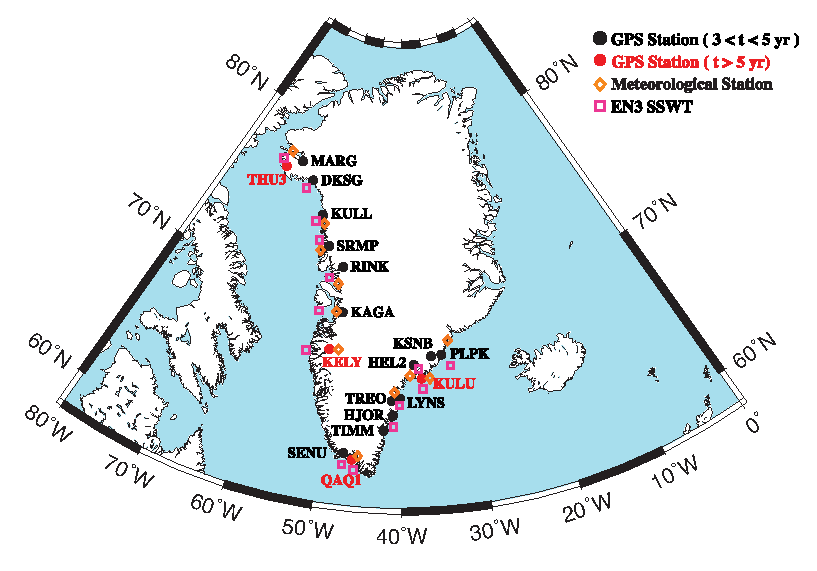
\includegraphics{figs_chpt3/2012GC004432-p01.eps} 
 \caption[Map of Greenland showing location of GPS sites, meteorological stations, and other data used in this study.]{Map of Greenland showing location of GPS sites, meteorological stations, and other data used in this study. Red circles indicate GPS sites with more than 5 years of data. Black circles indicate sites with 3 to 5 years of data. Orange diamonds indicate meteorological stations. Pink squares indicate pixels of sub-surface water temperature produced by EN3 model.}
 \label{fig:fig1}
\end{figure}

\clearpage
\begin{figure}
 \centering
 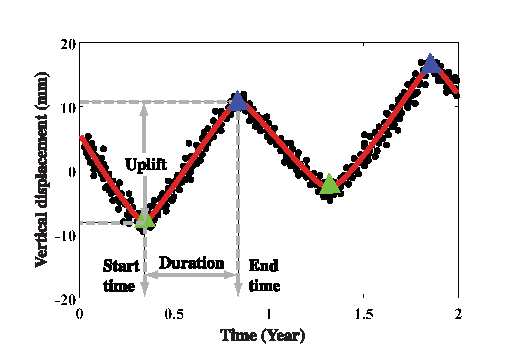
\includegraphics{figs_chpt3/2012GC004432-p02.eps} 
 \caption[Hypothetical 2 year time series showing four parameters (start time, end time, duration, and uplift) defined for a melt season.]{Hypothetical 2 year time series showing four parameters (start time, end time, duration, and uplift) defined for a melt season. Each black dot represents daily vertical position estimate. Red curve is best fit model. Blue triangles mark the maximum position value per year, and green triangles are the minimum value per year. A fifth parameter (rate of summer uplift) is the average slope of the curve between the start time and end time of uplift.}
 \label{fig:fig2}
\end{figure}

\clearpage
\begin{figure}
 \centering
 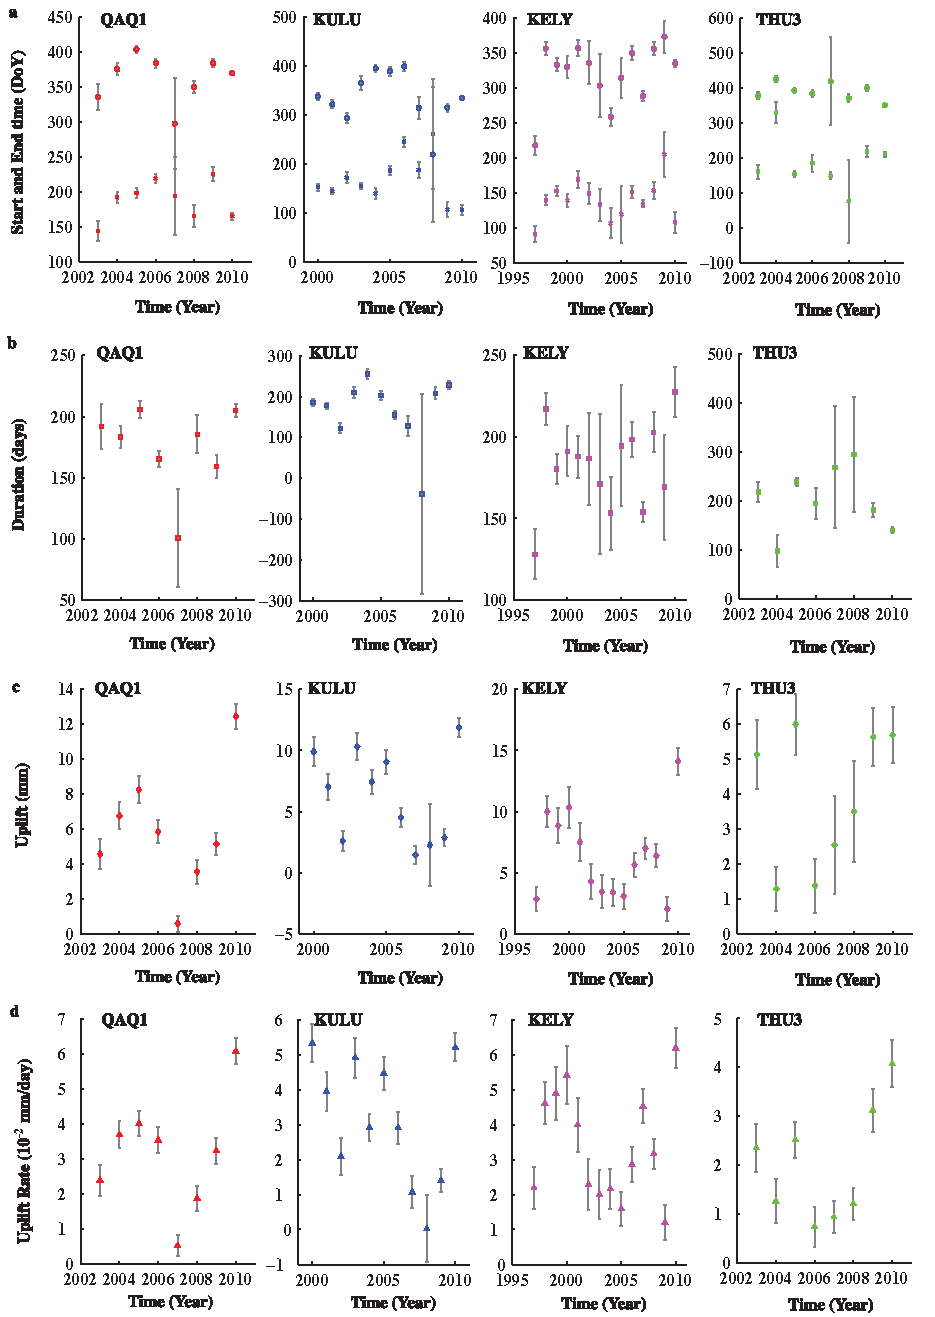
\includegraphics{figs_chpt3/2012GC004432-p03.pdf} 
 \caption[Annual variations of the five parameters defining seasonal uplift calculated for the four sites with longest observation record (red circles in Figure \ref{fig:fig1}).]{Annual variations of the five parameters defining seasonal uplift calculated for the four sites with longest observation record (red circles in Figure \ref{fig:fig1}). (a) Uplift start time (cross) and end time (circle), (b) uplift duration, (c) uplift magnitude, and (d) uplift rate. Gray line represents uncertainty.}
 \label{fig:fig3}
\end{figure}

\clearpage
\begin{figure}
 \centering
 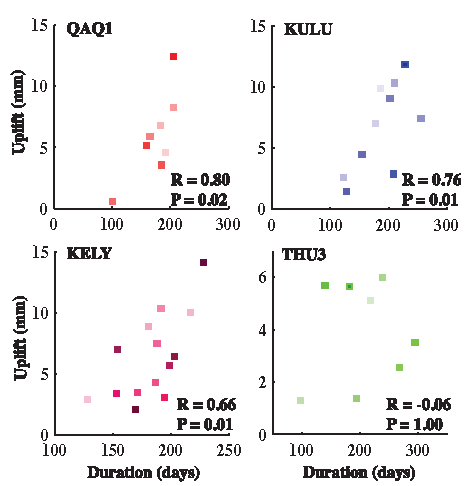
\includegraphics{figs_chpt3/2012GC004432-p04.pdf} 
 \caption[Uplift versus duration for the four sites with longest observation record.]{Uplift versus duration for the four sites with longest observation record. Colors varying from light to dark represent data from earlier to more recent.}
 \label{fig:fig4}
\end{figure}

\clearpage
\begin{figure}
 \centering
 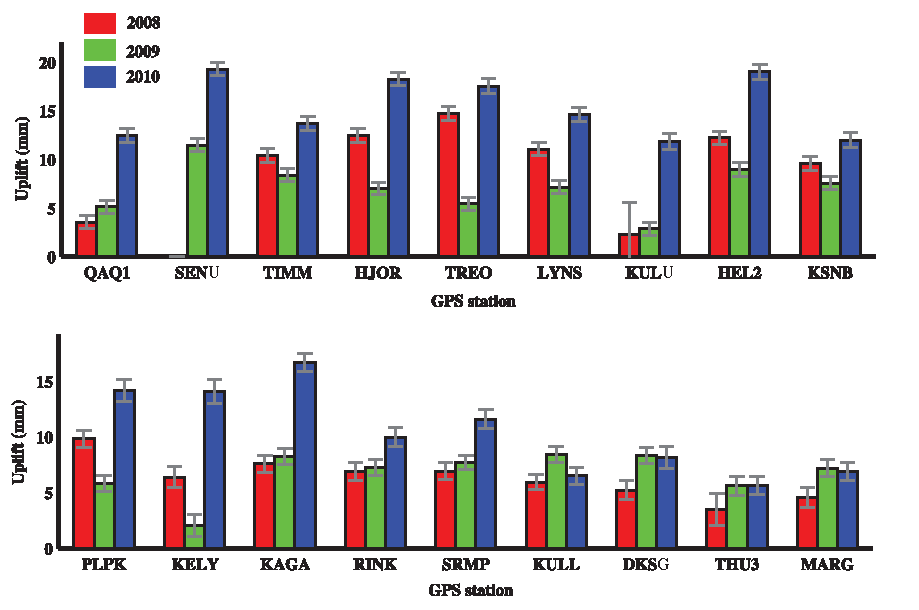
\includegraphics{figs_chpt3/2012GC004432-p05.pdf} 
 \caption[Seasonal uplift patterns for 2008–2010.]{Seasonal uplift patterns for 2008–2010. GPS sites are ordered by latitude, from south to north. Note change between KAGA (69.2 \textordmasculine N) and RINK (71.9 \textordmasculine N) with lower amplitude and lower variability uplift at the more northern sites.}
 \label{fig:fig5}
\end{figure}

\clearpage
\begin{figure}
 \centering
 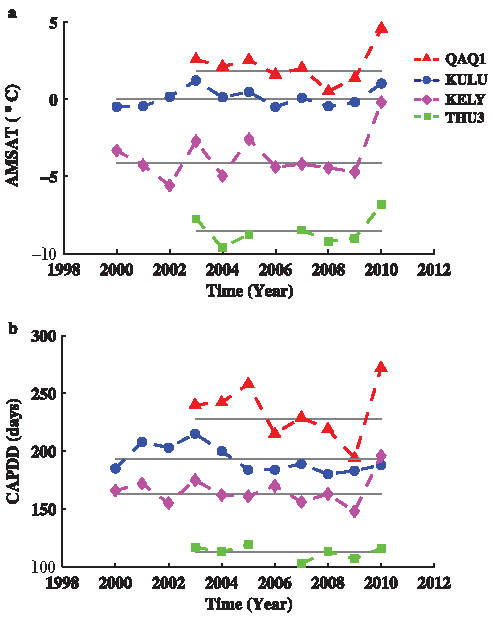
\includegraphics{figs_chpt3/2012GC004432-p06.pdf} 
 \caption[(a) AMSAT (Annual mean surface air temperature). (b) CAPDD (Cumulative annual positive degree days) for the four GPS stations with longest observation record.]{(a) AMSAT (Annual mean surface air temperature). (b) CAPDD (Cumulative annual positive degree days) for the four GPS stations with longest observation record. Solid gray line represents the mean value of reference period.}
 \label{fig:fig6}
\end{figure}

\clearpage
\begin{figure}
 \centering
 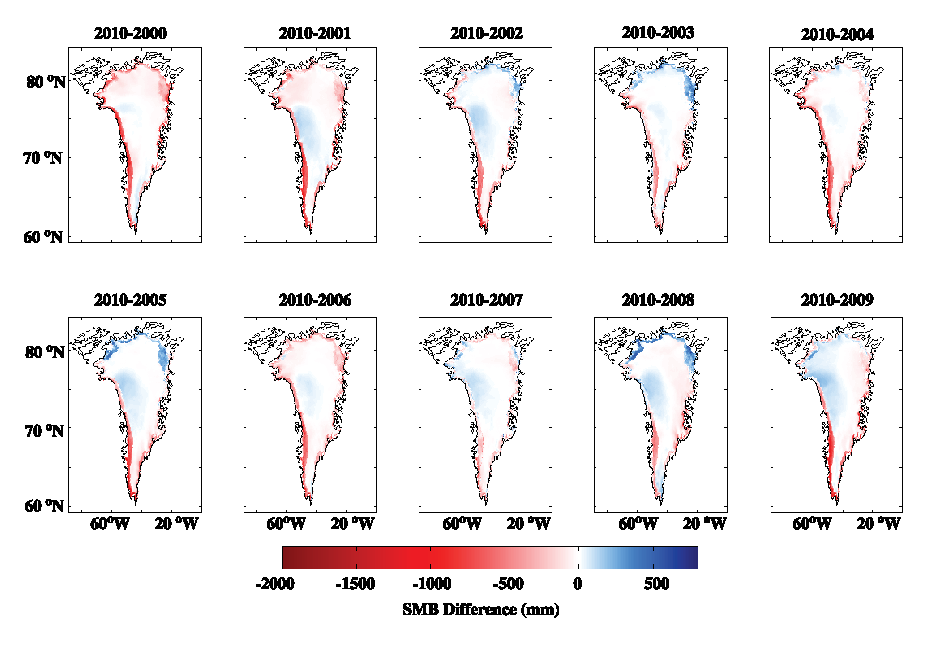
\includegraphics{figs_chpt3/2012GC004432-p07.eps} 
 \caption[Difference of Surface Mass Balance (SMB model from RACMO2) in summertime (June to August) between 2010 and 20XX (XX= 00–09) for the Greenland region.]{Difference of Surface Mass Balance (SMB model from RACMO2) in summertime (June to August) between 2010 and 20XX (XX= 00–09) for the Greenland region. Red color indicates that 2010 had a relatively negative SMB (more surface mass loss or less surface mass gain) compared to previous years, and blue color indicates that 2010 had a relatively positive SMB (less surface mass loss or more surface mass gain) compared to previous years.}
 \label{fig:fig7}
\end{figure}

\clearpage
\begin{figure}
 \centering
 \includegraphics{figs_chpt3/2012GC004432-p08.eps} 
 \caption[Difference of AMSSWT (Annual mean, sub-surface water temperature, depth range 5 m – 447 m) between 2010 and 20XX (XX = 00–09) for the Greenland region.]{Difference of AMSSWT (Annual mean, sub-surface water temperature, depth range 5m – 447 m) between 2010 and 20XX (XX = 00–09) for the Greenland region. Warmer colors indicate that 2010 was warmer than the previous year at a given location.}
 \label{fig:fig8}
\end{figure}

\clearpage
\begin{figure}
 \centering
 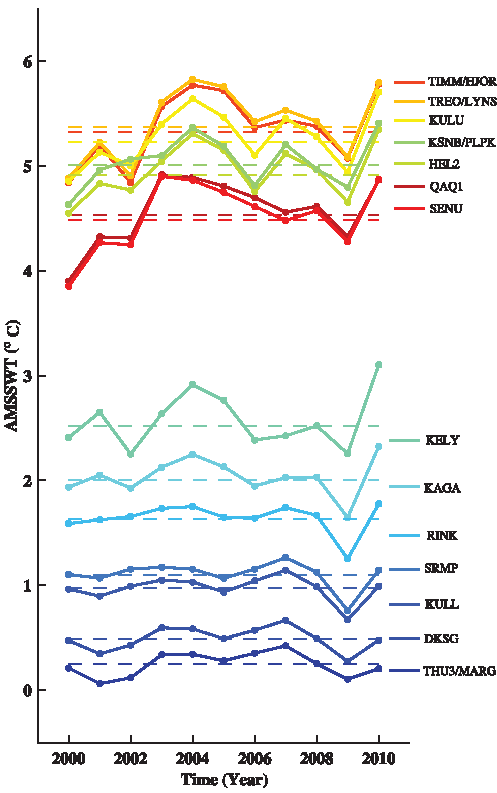
\includegraphics{figs_chpt3/2012GC004432-p09.pdf} 
 \caption[AMSSWT (Figure \ref{fig:fig8}) for “voxels” (model volume elements) nearest a given GPS station.]{AMSSWT (Figure \ref{fig:fig8}) for “voxels” (model volume elements) nearest a given GPS station. Warmer colors indicate southern latitudes, cooler colors indicate northern latitudes. Dashed color line represents 2000–2009 means. Note the pronounced 2010 anomaly for most locations, decreasing in intensity to the north.}
 \label{fig:fig9}
\end{figure}

\clearpage
\begin{figure}
 \centering
 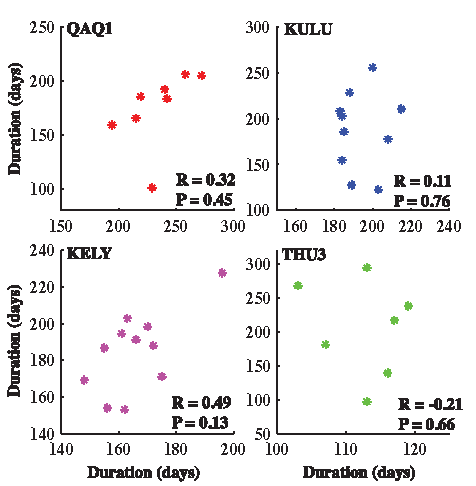
\includegraphics{figs_chpt3/2012GC004432-p10.pdf} 
 \caption{Uplift duration versus CAPDD (Figure \ref{fig:fig6}).}
 \label{fig:fig10}
\end{figure}

\clearpage
\begin{figure}
 \centering
 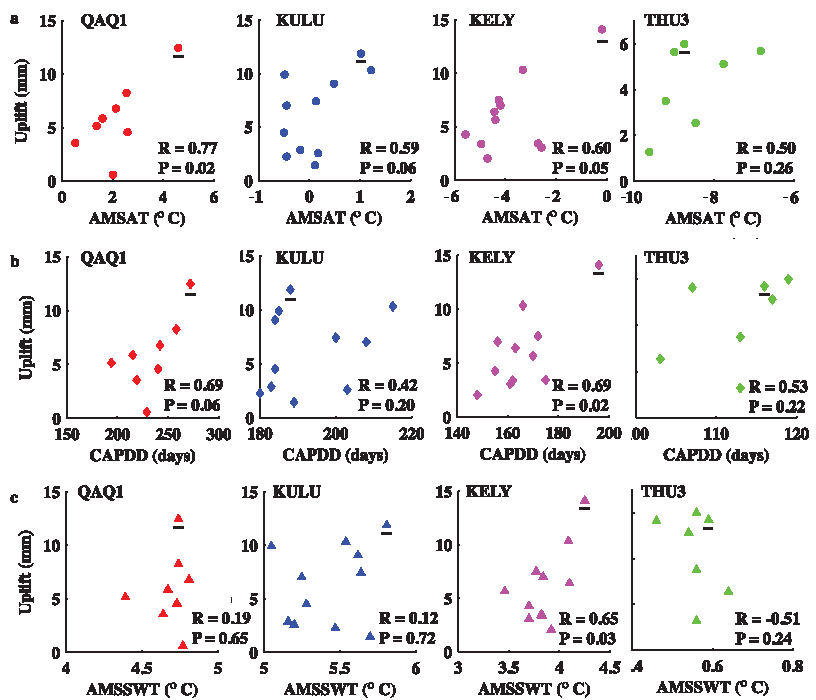
\includegraphics{figs_chpt3/2012GC004432-p11.pdf} 
 \caption[Spatial variation of seasonal uplift for four stations with longest time span related to (a) AMSAT (Figure \ref{fig:fig6}); (b) CAPDD (Figure \ref{fig:fig6}); and (c) AMSSWT (Figure \ref{fig:fig8}).]{Spatial variation of seasonal uplift for four stations with longest time span related to (a) AMSAT (Figure \ref{fig:fig6}); (b) CAPDD (Figure \ref{fig:fig6}); and (c) AMSSWT (Figure \ref{fig:fig8}). Underlined symbol is 2010.}
 \label{fig:fig11}
\end{figure}

\clearpage
\begin{figure}
 \centering
 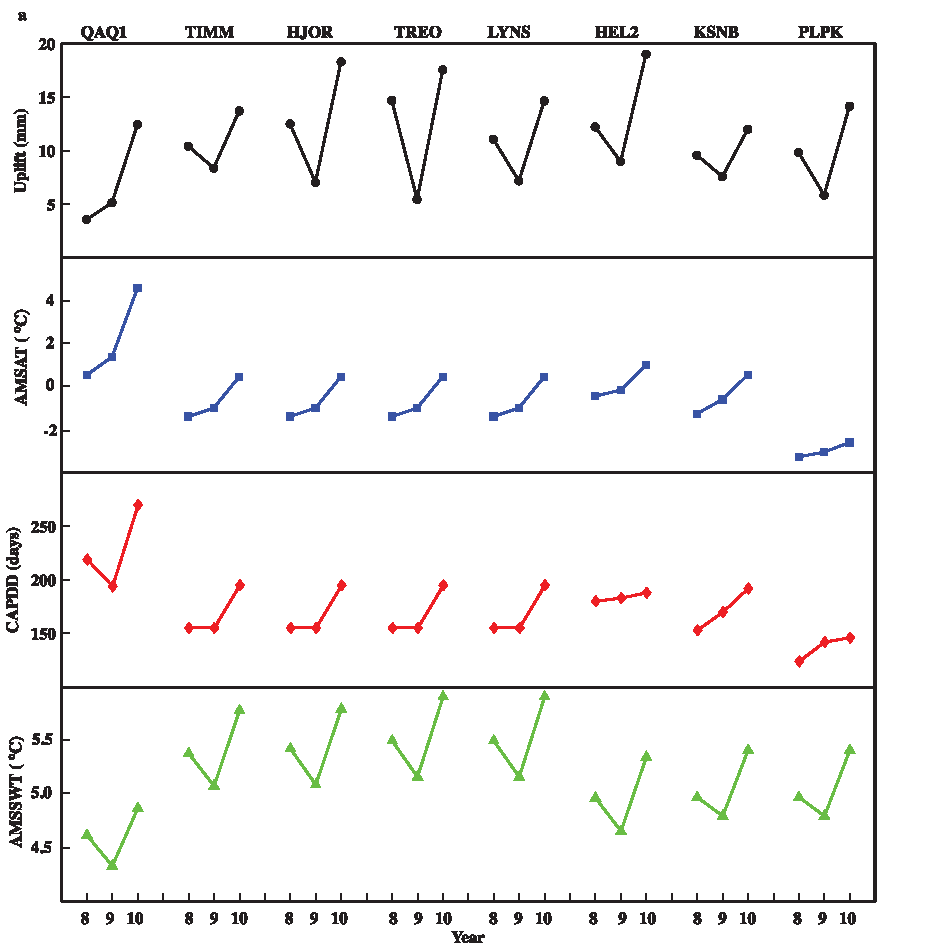
\includegraphics{figs_chpt3/2012GC004432-p12a.pdf} 
\end{figure}

\begin{figure}
 \centering
 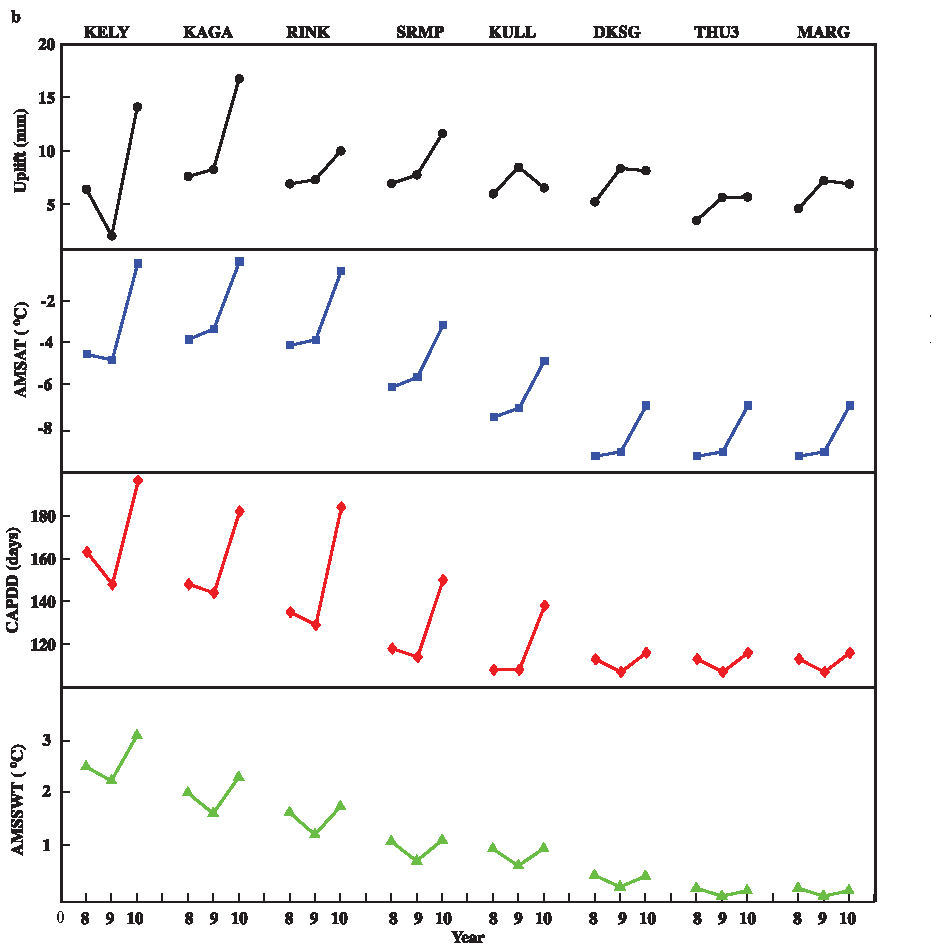
\includegraphics{figs_chpt3/2012GC004432-p12b.pdf} 
 \caption[Comparison between seasonal uplift patterns and atmospheric parameters (AMSAT and CAPDD, Figure \ref{fig:fig6}) as well as the ocean temperature parameter (AMSSWT, Figure \ref{fig:fig8}) for 2008–2010.]{Comparison between seasonal uplift patterns and atmospheric parameters (AMSAT and CAPDD, Figure \ref{fig:fig6}) as well as the ocean temperature parameter (AMSSWT, Figure \ref{fig:fig8}) for 2008–2010. Uplift pattern as shown in Figure \ref{fig:fig5}. SENU and KULU are eliminated here due to lack of data in 2008. GPS stations are ordered from south to north.}
 \label{fig:fig12}
\end{figure}

\clearpage
\begin{figure}
 \centering
 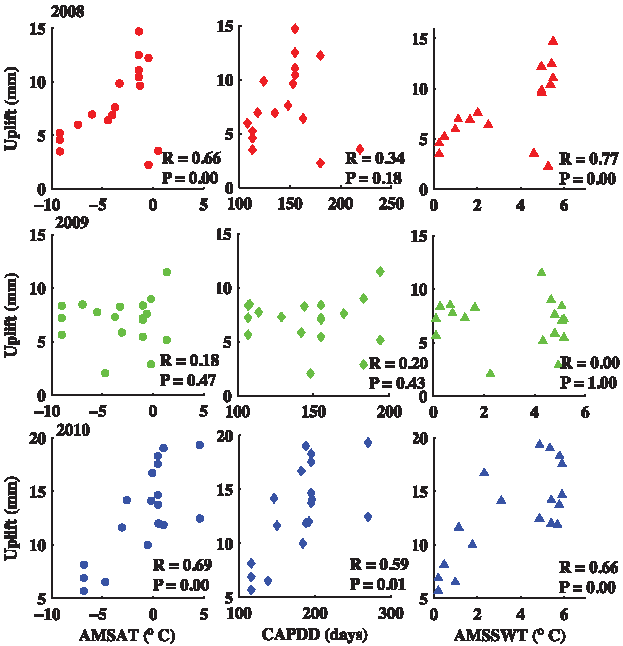
\includegraphics{figs_chpt3/2012GC004432-p13.pdf} 
 \caption{Temporal variation of seasonal uplift for all stations for 2008–2010 as a function of AMSAT
(Figure \ref{fig:fig6}), CAPDD (Figure \ref{fig:fig6}), and AMSSWT(Figure \ref{fig:fig8}).}
 \label{fig:fig13}
\end{figure}

\clearpage
\begin{figure}
 \centering
 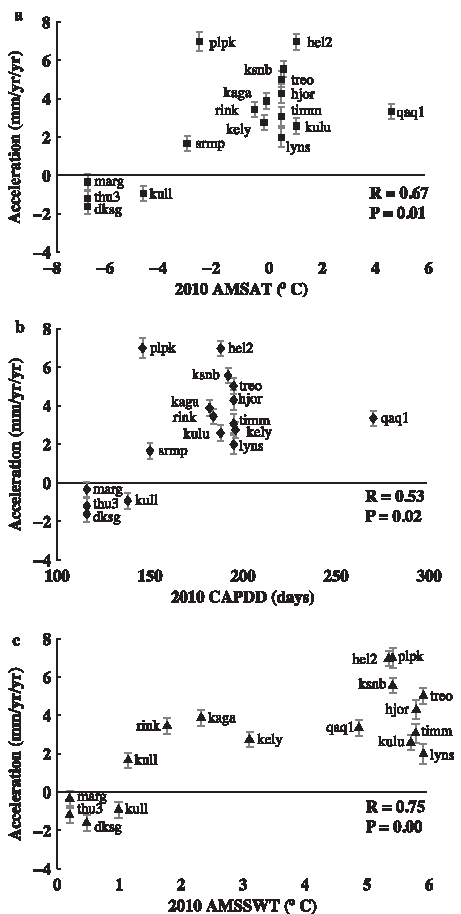
\includegraphics{figs_chpt3/2012GC004432-f14.pdf} 
 \caption{Spatial variation of uplift accelerations as a function of (a) AMSAT (Figure \ref{fig:fig6}), (b) CAPDD (Figure \ref{fig:fig6}), and (c) AMSSWT (Figure \ref{fig:fig8}) of 2010.}
 \label{fig:fig14}
\end{figure}

\clearpage
\begin{figure}
 \centering
 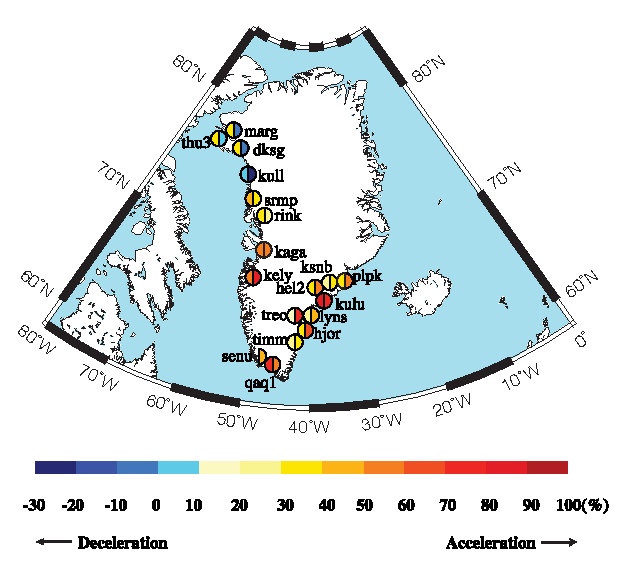
\includegraphics{figs_chpt3/2012GC004432-p15.pdf} 
 \caption[Site map of relative difference between uplift in 2010 and uplift in 2008 and 2009.]{Site map of relative difference between uplift in 2010 and uplift in 2008 and 2009. The left half circle shows percentage difference between the uplift in 2008 and 2010: $\triangle$U$_{10/08}$ = (U$_{10}$ - U$_{08}$)/U$_{10}$; right half circle shows percentage difference between uplift in 2009 and 2010: $\triangle$U$_{10/09}$ = (U$_{10}$ - U$_{09}$)/U$_{10}$.}
 \label{fig:fig15}
\end{figure}

\clearpage
\begin{figure}
 \centering
 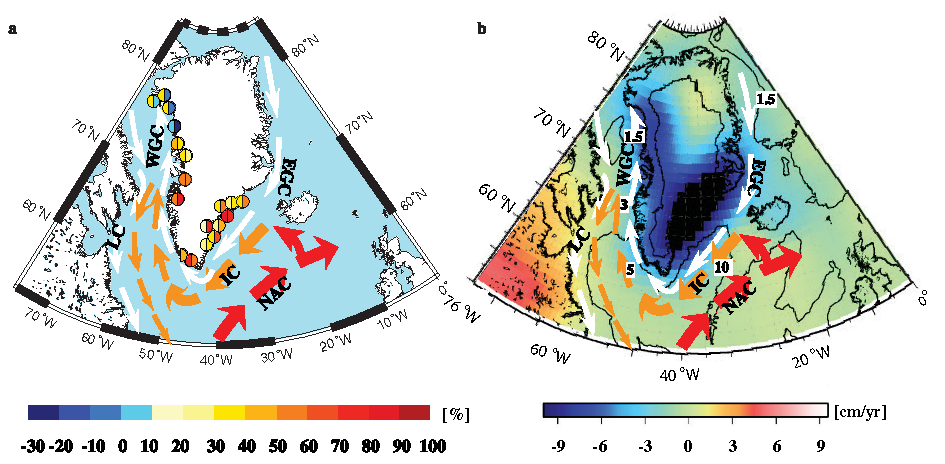
\includegraphics{figs_chpt3/2012GC004432-p16.pdf} 
 \caption[Relation between ocean currents, coastal uplift, and ice mass balance of coastal Greenland.]{Relation between ocean currents, coastal uplift, and ice mass balance of coastal Greenland. Red arrows indicate the mean path of the warm North Atlantic Current (NAC); orange arrows indicate Irminger Current (IC), white arrows indicate East Greenland Current (EGC), West Greenland Current (WGC) and Labrador Current (LC). (a) Relative difference between uplift in 2010 and that in 2008 and 2009 as shown in Figure 15. Names of GPS stations were omitted here. (b) Mass loss in equivalent water height over Greenland between February 2003 and January 2008 observed by GRACE \cite[]{wouters2008grace}. Numbers indicate the mean temperature (\textordmasculine C) of Atlantic-sourced waters on the Greenland shelf \cite[]{straneo2012characteristics}.}
 \label{fig:fig16}
\end{figure}
\chapter[Recent increases in Arctic freshwater flux affects Labrador Sea convection and Atlantic overturning circulation]{Recent increases in Arctic freshwater flux affects Labrador Sea convection and Atlantic overturning circulation \footnote{This chapter has been reprinted from Nature Communications with permission as: Yang, Q., Dixon, T. H., Myers, G. P., Bonin, J., Chambers, D., van den Broeke, M. R., (2016), Recent increases in Arctic freshwater flux affects Labrador Sea convection and Atlantic overturning circulation, Nat. Commun. 7:10525 doi: 10.1038/ncomms10525.}}

\section{Abstract}
The Atlantic Meridional Overturning Circulation (AMOC) is an important component of ocean thermohaline circulation.  Melting of Greenland’s ice sheet is freshening the North Atlantic, but whether the augmented freshwater flux is disrupting the AMOC is unclear.  Dense Labrador Sea Water (LSW), formed by winter cooling of saline North Atlantic water and subsequent convection, is a key component of the deep southward return flow of the AMOC.  Although LSW formation recently decreased, it also reached historically high values in the mid-1990s, making the connection to freshwater flux unclear.   Here we derive a new estimate of recent freshwater flux from Greenland using updated GRACE satellite data, present new flux estimates for heat and salt from the North Atlantic into the Labrador Sea, and explain recent variations in LSW formation.  We suggest that changes in LSW can be directly linked to recent freshening, and suggest a possible link to AMOC weakening.

\section{Introduction}
It has long been accepted that the AMOC has two stable modes \cite[]{stommel1961,rooth1982,broecker1985} and that anthropogenic warming could weaken or shut down the AMOC \cite[]{broecker1987,wood1999}.  Recent accelerated melting of the Greenland ice sheet is freshening the North Atlantic \cite[]{jiang2010,rignot2011,enderlin2014,velicogna2014regional,yang2013}.  So-called “hosing experiments”, where freshwater may be distributed over broad or narrow regions of the North Atlantic in numerical models, have been used to study the sensitivity of the AMOC to freshwater flux \cite{fichefet2003,jungclaus2006,stouffer2006,hu2011,swingedow2013,ridley2005,brunnabend2015}.  Some of these studies suggest that AMOC strength is sensitive to Greenland melting \cite[]{fichefet2003,brunnabend2015} while others do not \cite[]{jungclaus2006,hu2011,ridley2005}.  A few studies suggest that freshwater additions of 0.1 Sv (100 mSv) \cite[]{rahmstorf1995,rahmstorf2005,hawkins2011} or possibly less \cite[]{fichefet2003,brunnabend2015}could affect the AMOC. 

Changes in the AMOC are difficult to measure directly: currents that comprise the deeper, southward flowing portions can be diffuse and/or spatially and temporally variable, and instrumental drift can mask subtle, long term changes in oceanic properties.  It is also challenging to separate changes forced by anthropogenic warming from natural variability.  The AMOC is difficult to model numerically: model grids may be too coarse to reflect realistic oceanic processes and geographic constraints, and feedbacks among atmosphere, ocean and cryosphere (land and sea ice) are poorly known. 

The Labrador Sea is a key location for the formation of one of the dense, deep water components of the AMOC via winter convection, but the process is sensitive to surface conditions \cite[]{yashayaev2009}.  \citet{wood1999} suggest the possibility of a shutdown in Labrador Sea convection in response to global warming.  \citet{kuhlbrodt2001} provide a theoretical stability analysis, and suggest that winter convection in the Labrador Sea can be turned off by increased freshwater input. Unfortunately, winter convection here is difficult to observe directly due to extreme conditions and its small spatial scale. 

Here we consider recent Labrador Sea changes associated with increased freshwater flux.  We derive a new estimate for recent increased freshwater flux into the sub-polar North Atlantic, and suggest that because of the clockwise nature of ocean circulation around Greenland \cite[]{joyce2007}, most of this increase is being focused towards the Labrador Sea (Figure \ref{fig:chpt4_fig1}), magnifying its impact and increasing the likelihood of significant effects on the AMOC.

\section{Results}
\subsection{Recent accelerated melting of the Greenland ice sheet}
Numerous studies have described recent acceleration of Greenland’s ice mass loss \cite[]{jiang2010,rignot2011,enderlin2014,velicogna2014regional,yang2013}.  We use GRACE data updated to October 2014 to derive a new acceleration estimate and its onset time (Methods).  GRACE data and uncertainty estimates follow \citet{bonin2013}.  We fit a constant acceleration model to the data, and extrapolate the best-fit model back to the time of zero mass loss rate, obtaining 20 Gt yr$^{-2}$ acceleration with a start time of 1996 $\pm$ 1.4 years (Figure \ref{fig:chpt4_fig2}).  Several lines of evidence suggest that the ice sheet was relatively stable from 1980 to the early 1990s \cite[]{howat2011,box2013}, and we use that assumption in our modeling of GRACE data and freshwater flux calculations (below and Methods section). 

\subsection{Irminger Water heat and salt fluxes}
Warming of sub-polar mode waters including Irminger Water in the mid- to late-1990s \cite[]{myers2007b,thierry2008}is thought to influence coastal mass loss in Greenland by increasing submarine melting of outlet glaciers and related dynamic effects \cite[]{holland2008,joughin2012,straneo2013}.  Here, we examine the variability of heat and salt fluxes of Irminger Water along three sections (Figure \ref{fig:chpt4_fig1}) offshore southwest coastal Greenland for the period 1949 – 2013 (Methods).  Currents associated with the sub-polar gyre here are quite compact as they round the southern tip of Greenland, limiting spatial variability and facilitating accurate flux measurements, because the cross section area of current is well defined.  Note that while flux (sensu stricto) is flow rate per unit area, and transport (or total flux) represents the flux integrated over the larger area of interest, the terms “flux” and “ transport” are often used interchangeably in the oceanographic literature.  We follow the broader (sensu lato) usage here.  

We carry out our analysis on the upper 700 m, the greatest depth common to all years, binned on a 2 m vertical grid.   Time series of heat flux and salt flux at the three sections are shown in Figure \ref{fig:chpt4_fig3}.  At the southernmost Cape Farewell section, both heat flux and salt flux experienced a large multi-year anomaly around 1995, followed by another in the late 1990s.  The heat flux was 80\% higher than a previous multi-year anomaly in the 1960s.  Similar variability is seen at the more northerly Cape Desolation section, although salinities and heat are generally lower, and only exceed previous levels after 2000.  No significant anomalies were observed at the northernmost Paamiut section during these times, but the heat and salt fluxes are still roughly 50\% higher after 2000 than they were in the 1980s, and approach levels not seen since the 1960s. Thus, we conclude that Irminger Water became warmer and saltier in the mid-late 1990s, which agrees well with the onset time of recent accelerated Greenland mass loss (Figure \ref{fig:chpt4_fig2}2).  This is consistent with the idea that accelerating ice mass loss in the mid-late 1990s reflects, at least in part, the appearance of warmer Irminger Water on the peripheral continental shelf at that time \cite[]{holland2008}.  The anomalous heat flux we observe off southern Greenland in the mid-1990s can be directly tied to warming of the North Atlantic (Figure \ref{fig:SI4_fig2}; see also \citet{straneo2013}). 

Northward reduction in heat and salt transport between the Cape Desolation and Paamiut sections likely reflects strong offshore eddy transport \cite[]{jakobsen2003}, advecting Irminger Water into the interior of the Labrador Sea.   However, since the sections are only occupied once a year in summer, some seasonal aliasing is possible.  The eddies also transport fresh shelf water into the Labrador Sea \cite[]{myers2009}. 
  
\subsection{Estimates of freshwater flux into the Labrador Sea}
Major sources of freshwater entering the Labrador Sea include precipitation, oceanic transport, and melt from the Greenland ice sheet, glaciers in the Canadian Arctic Archipelago (CAA) and Arctic sea ice. Precipitation in the Labrador Sea region is about 20 – 30 mSv \cite[]{myers2007a} , and there has been a general increase over the North Atlantic region in the last few decades as the hydrologic cycle accelerates \cite[]{josey2005}.  Oceanic transport from the Arctic Ocean is the largest source of Labrador Sea freshwater, and is derived from several sources, including the difference between precipitation and evaporation, river discharge, and fractionation associated with annual sea ice formation.  \citet{peterson2002} show that the average annual river discharge from six rivers in Eurasia into the Arctic Ocean has increased by 7\% ($\sim$4 mSv) from 1936 to 1999.  The Arctic Ocean exports low salinity water to the North Atlantic through two main pathways: Fram Strait east of Greenland, and the CAA west of Greenland.  The CAA pathway has three main routes: Barrow Strait, Nares Strait, and Cardigan Strait-Hell Gate.  Roughly 100 mSv of freshwater is exported through each of the east and west pathways, relative to a reference salinity of 34.80 \cite[]{haine2015}.  Within broad error bars, oceanic transport from the Arctic Ocean is relatively stable on the decadal time scale, although there has been some reduction through the CAA and then Davis Strait, and shorter term fluctuations are common \cite[]{haine2015,castro2015,curry2014}.  

Here we focus on three Arctic freshwater sources that are undergoing rapid increases, that likely contribute freshwater to the Labrador Sea, and that can be estimated from remote observations: the Greenland ice sheet, CAA glaciers, and Arctic sea ice.  We also consider snowmelt runoff from tundra in Greenland and the CAA as they follow directly from the same models used to quantify Greenland ice sheet and CAA glacier melt \cite[]{bamber2012,lenaerts2013}.  As we are not considering the large Arctic oceanic transport term and several other sources, our estimate is a minimum estimate.

Freshwater flux from Greenland is composed of ice and tundra runoff plus ice discharge; this quantity is equal to accumulation minus mass balance (Methods).  We derive mass balance for Greenland from GRACE, while accumulation is obtained from the RACMO2.3 model \cite{ettema2009,noel2015}.  Our GRACE data suggest that mass loss of the Greenland ice sheet accelerates from 1996 onward (Figure \ref{fig:chpt4_fig2},  Methods).  Our mass balance estimate agrees with the estimate of Box and Colgan26, with the Greenland ice sheet in near balance from 1980 to about 1996, after which it starts to lose mass (Figure \ref{fig:chpt4_fig3}).  Therefore, we assume that between 1980 and 1996, freshwater flux from Greenland is approximately equal to accumulation;  after 1996, freshwater flux from Greenland equals the sum of mass loss and accumulation (Figure \ref{fig:chpt4_fig3}).  Since the accumulation is highly variable from year to year, we smooth it with a 5-year running mean.  Figure 4 shows the resulting freshwater flux estimates from Greenland.  This approach yields freshwater flux estimates that agree  with those of \citet{bamber2012} during the period of data overlap, once a correction for solid ice discharge is applied8 (Figure \ref{fig:chpt4_fig4}).  Freshwater from the CAA is approximated by ice and tundra runoff predicted by RACMO2.3 since ice discharge (0.16 mSv) is negligible \cite[]{gardner2011}.  

Large amounts of Arctic sea ice and freshwater are exported from the Arctic Ocean to the North Atlantic through several pathways.  Of these, Fram Strait and the CAA are the major ones; nearly all ($\sim$98\%) Arctic Ocean export drains through them \cite[]{haine2015}. However, there are large uncertainties in these fluxes \cite[]{haine2015}.  We focus on changes in freshwater flux as inferred from recent accelerated melting of Arctic sea ice, assuming that the change is partitioned the same way as total export, i.e., 98\% of the change is advected through Fram Strait and the CAA.  Changes in the annual minimum of Arctic sea ice volume are a relevant indicator (see Methods and Appendix B).  We first use the annual minimum volume predicted by the Pan-Arctic Ice Ocean Modeling and Assimilation System (PIOMAS) model \cite[]{zhang2003}.   We also apply the same method to the Arctic sea ice extent and sea ice area data sets \cite[]{fetterer2002}, where “extent” defines a region as either “ice-covered” or “not ice-covered” using a threshold of 15\%; “area” is a more conservative estimate, defined as the percentage of actual sea ice within a given data cell.  We assume a standard ice thickness of 2 m \cite[]{laxon2003} to convert ice extent and ice area to volume, obtaining results that are somewhat smaller than the PIOMAS volume model.  Figure \ref{fig:chpt4_fig4} shows results from the PIOMAS volume model.  Results from the other two approaches are shown in Figures \ref{fig:SI4_fig5} and \ref{fig:SI4_fig6}.  

Figure 4 also shows the summed result from these various freshwater sources (recall that this summed value does not include several major sources and is therefore a minimum estimate), which is our estimate of the freshwater flux into the sub-polar North Atlantic. Freshwater flux from Greenland is relatively stable from 1979 to the mid-late 1990s and then increases.  Freshwater flux from the CAA is relatively stable until the early 2000s and then increases.  Freshwater flux from Arctic sea ice increases mainly during the period 1990 to 2000.  The total freshwater flux for the sub-polar North Atlantic from these sources is about 60 mSv by 2013 with an increase of 20 mSv during the last two decades. Of this $\sim$12 mSv comes from the Greenland ice sheet and CAA glaciers, while $\sim$8 mSv represents excess melting of Arctic sea ice. 

Focused freshwater flux into the Labrador Sea has the potential to disrupt the AMOC by increasing the buoyancy of surface waters and reducing the formation of dense, deep water \cite[]{stouffer2006}. How much of the enhanced freshwater flux that we calculate actually winds up in the Labrador Sea?

\citet{myers2009,myers2005} showed that a significant fraction of freshwater originating in and around Greenland is transported to the Labrador Sea: melt water from eastern Greenland is entrained in the East Greenland Current, where it moves south and merges with the Irminger Current as it rounds Cape Farewell; melt water from southwestern Greenland joins the West Greenland Current, similarly merging with the Irminger Current (Figure \ref{fig:chpt4_fig1}).  Meltwater from the CAA enters the Labrador Sea through Davis and Hudson straits, either directly or indirectly \cite[]{mcgeehan2012}.  The pattern of boundary currents and eddy activity around Greenland and Labrador insures that at least 75 percent of the freshwater flux from the Greenland ice sheet and CAA eventually winds up in the Labrador Sea (Appendix B).  Freshwater and sea ice drained from the Arctic Ocean moves south through Fram Strait and the CAA37, also contributing to freshening of the Labrador Sea both remotely and locally \cite[]{koenigk2006,peterson2006}.  We estimate that at least 65 percent of freshwater and sea ice exported from the Arctic Ocean through Fram Strait and the CAA ultimately makes it to the Labrador Sea (Appendix B).  Assuming these estimates are correct, of the 20 mSv freshwater flux increase that we estimate, at least 14mSv (70\%) winds up in the Labrador Sea (Appendix B).  Given typical coastal current velocities, most of this freshwater is transported to the Labrador Sea within 3 - 12 months.  Some freshwater from the CAA may take 2 – 3 years to reach the Labrador Sea due to recirculation and storage in Baffin Bay and/or recirculation in the sub-polar gyre. 

\subsection{Impact of increased freshwater flux on deep water formation}
To investigate effects of increased freshwater flux on deep water formation in the Labrador Sea, we can either look at the mean density of LSW within a given depth range, or look at the thickness of LSW as defined by a given density range.  We used both approaches, obtaining similar results. Figure \ref{fig:chpt4_fig5} shows results from the second approach, where we calculate the thickness of LSW, defined by   kg m$^{-3}$, from 1950 to 2013, using the objective analyses of the EN4.0.2 data set from the UK Met Office Hadley Center \cite[]{good2013}.  The data set includes monthly temperature and salinity with a spatial resolution of 1 $\textordmasculine$ $\times$ 1 $\textordmasculine$ and 42 depth intervals (5 m to 5350 m) from 1900 to present.  Results for density over a fixed depth range (1000 m – 2500 m) are shown in Figure \ref{fig:SI4_fig8}.
  
Figure \ref{fig:chpt4_fig5} shows the time series of LSW thickness, compared to our estimate of freshwater flux and to the Irminger salt flux time series.  From 1950 to the mid-1990s, Irminger salt flux and LSW thickness are weakly correlated ($R$ = 0.3, $P$ = 0.03), and both show multidecadal oscillations, with highs in the 1960s, lows in the 1980s, and highs in the 1990s.  In particular, LSW thickness increased significantly (by 65\%) between 1990 and 1995 when salt flux increased, consistent with the idea that dense deep water in the Labrador Sea originates from warm, saline North Atlantic water that subsequently experiences winter cooling.  However, this relationship begins to break down in the mid-to-late 1990s, when freshwater flux from Greenland and other sources increased rapidly.  Since then, LSW thickness decreased continuously, reaching lows not observed since the early 1970s, despite continued high salt flux.  One interpretation of this is that increased freshwater flux has now overwhelmed increased salt flux from the Atlantic, and has begun to influence LSW formation.  Recall that increased salt flux from the Atlantic is accompanied by increased heat flux (Figure \ref{fig:chpt4_fig3}) which promotes melting of marine-terminating outlet glaciers in southern Greenland \cite[]{holland2008,rignot2006}, and increased freshwater flux.  

Our data are consistent with recent studies showing a decline in the thickness of the dense mode of LSW since 1994/95, with a switch to a less dense and presumably fresher and warmer upper mode \cite{rhein2011,kieke2015}. \citet{yashayaev2015} show declining upper salinity since the mid-2000s and suggest that salinity is the controlling factor for ocean stratification in this region.  Declining upper layer salinity would weaken or even prevent Labrador Sea convection.  However, cold winter air also plays a role in LSW formation.  Severe winter conditions and strong air-sea heat exchange for the period 1990 – 1995 may have contributed to the increased LSW thickness \cite[]{lazier2002}, while milder winter conditions and weaker cooling since 1995 may have contributed to LSW decline \cite{vage2009}.  The Labrador Sea is also sensitive to multidecadal climate variations.  Hydrographic properties in the Labrador Sea exhibit multidecadal variability that resemble the Atlantic Multidecadal Oscillation (AMO) and the North Atlantic Oscillation (NAO) \cite[]{yashayaev2015}, and these variations are obvious in the flux (Figure \ref{fig:chpt4_fig3}) and LSW thickness (Figure \ref{fig:chpt4_fig5}) time series.  Bidecadal variability in the Labrador Sea forced by volcanic activity has also been proposed \cite[]{swingedouw2015}.  Despite these complications, our data clearly show a steep, recent increase in freshwater flux into the Labrador Sea and a steep decline in LSW thickness (and density) at the same time (Figure \ref{fig:chpt4_fig5}), which is inconsistent with the estimated salt flux into the region.  This suggests a potential impact on formation of North Atlantic Deep Water.  

\section{Discussion}
Our reconstructed annual freshwater flux for the sub-polar North Atlantic reaches 60 mSv in 2013 with an increase of 20 mSv in the last two decades (Figure \ref{fig:chpt4_fig4}).  At least 70 percent (14 mSv) of this increased freshwater is focused towards the Labrador Sea (Appendix B).  This is a minimum estimate since we do not consider other major sources.  LSW formation may reflect a delicate balance between this cold freshwater and warm, salty North Atlantic water from the Irminger Current.  The flux of freshwater from Greenland may in turn be influenced by warm Atlantic water and its influence on the regional ocean and atmosphere, a potentially important feedback in the system.  

Since LSW is an important component of the dense southward return flow of the AMOC, factors influencing LSW formation may in turn impact the AMOC.  Hosing experiments show different sensitivities of the AMOC to freshwater fluxes at high latitudes \cite[]{fichefet2003,jungclaus2006,stouffer2006,hu2011,swingedow2013,ridley2005,brunnabend2015}11-17.  \citet{hu2011} suggest that freshwater inputs much larger than we observe are required.  On the other hand, \citet{fichefet2003} suggest that freshwater flux anomalies as small as 15 mSv will affect the AMOC.   \citet{brunnabend2015} suggest that freshwater flux anomalies as small as 7 mSv applied over 30 years could impact the AMOC.  Different model outcomes partly reflect their spatial resolution, the degree to which freshwater fluxes are focused towards the Labrador Sea, and the time scale over which anomalous flux is applied.  \citet{swingedow2013} compared different model responses to freshwater release around Greenland, assuming freshwater focusing into the Labrador Sea.  They show significant AMOC weakening after several decades with a flux anomaly of 100 mSv.

If our inference that the sub-polar gyre’s coastal currents focus melt water from Greenland, CAA glaciers and Arctic sea ice into the Labrador Sea is correct, then present rates of increased freshwater flux may be sufficient to influence convection in the Labrador Sea and by implication the AMOC. Northward decreases in heat and salt flux across our three sections in southwest Greenland indicate strong mixing of coastal water and westward advection into the Labrador Sea.  Eddy kinetic energy reaches a local maximum offshore Cape Desolation and Paamiut, where a front develops between Irminger Water and fresh shelf water, promoting baroclinic instability and eddy formation; these eddies propagate westward into the Labrador Sea.  Local bathymetric structures, especially the sill at Davis Strait, also promote westward propagation of coastal water from southwestern Greenland.  Recent high-resolution eddy permitting or eddy-resolving numerical models support this type of spatial focusing, and indicate decline or even shutdown of Labrador Sea convection with enhanced freshwater flux from Greenland \cite[]{weijer2012} or from the Arctic Ocean through the CAA \cite[]{mcgeehan2011}.   Since freshwater lenses can retain their integrity for some time, “temporal focusing” may also be important.  Summer (June, July, August) freshwater fluxes from Greenland and CAA’s ice and snow runoff greatly exceed the annual mean. Summer freshwater flux from Greenland and the CAA increased by about 50 mSv from mid-late 1990s to 2013, reaching a high of 150 mSv in 2012 (Figure \ref{fig:SI4_fig9}), potentially limiting convection during the subsequent winter. 

We suggest that recent freshening in the vicinity of Greenland is reducing formation of dense LSW, potentially weakening the AMOC.   Recent observations are beginning to document declines in the AMOC \cite[]{robson2013,smeed2014,rahmstorf2015}, consistent with our hypothesis.  Longer time series will be required to confirm this link, but our preliminary results suggest that detailed studies of Labrador Sea hydrography and proximal sources of freshwater, including Greenland, have the potential to improve our understanding of AMOC variability and sensitivity to anthropogenic warming.
 
\section{Methods}
\subsection{GRACE data}
The GRACE time series were created via the least squares inversion method described in \citet{bonin2013}.  Release-05 GRACE data from the Center for Space Research (CSR) were used, with the standard post-processing applied as described in that paper: C20 is replaced by Satellite Laser Ranging (SLR) estimates, a geocenter model is added, GIA is corrected for, and the monthly averages of the Atmosphere and Ocean Dealiasing (AOD) product are restored.

The inversion technique is designed to localize the mass change signal, such that coastal mass loss from Greenland does not leak into the ocean or into interior Greenland due to GRACE’s inherently low spatial resolution.  Briefly, the method involves breaking Greenland and the surrounding area into pre-defined regions (Greenland drainage basins; Figure \ref{fig:SI4_fig10}).  Each region is assumed to have a uniform mass distribution when gridded as 1 $\textordmasculine$ $\times$ 1 $\textordmasculine$-binned kernels.  The transformation to degree/order 60 spherical harmonics is then made upon each individual regional kernel, resulting in a smoothed version of each region that mimics what GRACE would see from its limited resolution, if a uniform mass of 1 was placed over the kernel, with zeroes elsewhere.

The goal is to find a set of multipliers for each region which most closely describes mass distribution over Greenland, given the assumption of uniform weights across each pre-defined shape.  A least squares method is used to fit an optimal multiplier to each basin simulataneously, such that the combination of the multipliers times the smoothed basin kernels best fits the actual (smoothed) GRACE data for that month.  An optimal amount of process noise is added to stabilize the solution \cite[]{bonin2013}. 

The GRACE mass balance in this paper is the sum of the individual signals from the 16 Greenland regions (Figure \ref{fig:SI4_fig10}).

\subsection{Irminger Water heat and salt flux analysis}
Details of the data collection and analysis are discussed in \citet{myers2007b} and summarized here.  Prior to 1984 the estimates are based on a climatological analysis of the Labrador Sea.  The 1984 – 2013 observations are collected on a set of standard sections by the Danish Meteorological Institute.   Each section (Figure \ref{fig:chpt4_fig1}) involves the same 5 stations, but in some years only 3 or 4 stations could be occupied.  The sections are occupied annually in most years, in late June or early July.  Direct sampling using bottles was performed in 1984-87, while CTD (Conductivity-Temperature-Depth) data were collected in later years.  We carry out our analysis on the upper 700 m, the deepest depth common to all years, binned on a 2 m vertical grid.  For current motions, we determine the geostrophic velocity, relative to 700 dbar ($\sim$700 m depth) or the bottom in shallower water, for each pair of stations at each depth, and add an estimate of the barotropic velocity \cite[]{myers2009}.  If data are missing, we do not include that point in the calculation.  We calculate heat flux (\textit{Q}$_{\V{t}}$) and salt flux (\textit{Q}$_{\V{s}}$) at each depth and then sum those whose temperature and salinity are consistent with Irminger Water to obtain the total transport:
\begin{equation}
\begin{aligned}
Q_{\V{t}}=\rho \cdot C_{\V{p}} \cdot \int_{s=1}^{s=5} \int_{z=-700}^{z=0} \upsilon(s,z) \cdot (T(s,z)-T_{\V{ref}})dzds
\end{aligned} 
\end{equation} 

\begin{equation}
\begin{aligned}
Q_{\V{s}}=\int_{s=1}^{s=5} \int_{z=-700}^{z=0} \upsilon(s,z) \cdot (S(s,z)-S_{\V{ref}})dzds
\end{aligned} 
\end{equation}
where $\rho$ and $C_{\V{p}}$ are ocean water density and heat capacity respectively, $\upsilon(s,z)$,$T(s,z)$ and $S(s,z)$ are velocity, temperature and salinity in station $s$ at depth $z$ respectively, $T_{\V{ref}}$ is the reference temperature (0 \textordmasculine C) and $S_{\V{ref}}$ is the reference salinity(34.80).  Here, we choose a broad definition including both pure and modified Irminger Water, with temperature warmer than 3.5 \textordmasculine C and salinity higher than 34.88 \cite[]{myers2007b}.

\subsection{Freshwater flux}
To estimate the freshwater flux from Greenland, we first use a simple constant acceleration model to fit the monthly GRACE mass balance data:  
\begin{equation}
\begin{aligned}
M(t_{i})=a+bt_{i}+\frac{1}{2}ct_{i}^{2}
\end{aligned} 
\end{equation}
where $M(t_{i})$ ($i$=1,2,3...n) are GRACE monthly solutions, $a$ is the initial mass of Greenland, $b$ is the initial mass balance, and $c$ is the acceleration term.  Given the estimated parameters, the mass balance ($MB$) of Greenland can be represented by:
\begin{equation}
\begin{aligned}
MB(t_{i})=b+ct_{i}
\end{aligned} 
\end{equation}
The start time of recent accelerated mass loss is the time $t_{i}$ when $MB(t_{i})$ is zero.  The mass balance of Greenland is:
\begin{equation}
\begin{aligned}
MB=SMB-D
\end{aligned} 
\end{equation}
where $SMB$ is surface mass balance and $D$ is discharge, related to freshwater flux ($FWF$) by:
\begin{equation}
\begin{aligned}
SMB=A-R
\end{aligned} 
\end{equation}
\begin{equation}
\begin{aligned}
FWF=R+D
\end{aligned} 
\end{equation}
where $A$ is the accumulation and $R$ is runoff.

We then calculate freshwater flux from Greenland using the above relations, rewriting them as:
\begin{equation}
\begin{aligned}
FWF=A-MB
\end{aligned} 
\end{equation}
where accumulation ($A$) is predicted by RACMO2.3 and mass balance ($MB$) is estimated from the GRACE data.  Note that accumulation is defined over ice and tundra and mass balance is the total mass balance of Greenland, including ice and tundra.  Therefore, freshwater flux from Greenland is composed of ice mass loss and tundra runoff (Figure \ref{fig:SI4_fig11}).  Mass balance is considered equal to zero prior to the recent acceleration phase, beginning in 1996.  Since mass balance is the long-term average, accumulation is smoothed with 5-year running average.

For the CAA, we assume $FWF=R$ when estimating freshwater flux since ice discharge from the CAA is negligible compared to runoff \cite[]{gardner2011}. Thus, freshwater flux from the CAA is derived from runoff predicted by RACMO2.3.  Note that both ice runoff and tundra runoff are considered in the freshwater flux calculation (Figure \ref{fig:SI4_fig12}).

For Arctic sea ice, we focus just on recent accelerated melting of multi-year ice, which results in loss of ice area and extent, rather than the much larger contribution from the annual freeze-thaw cycle, which forms significant freshwater through fractionation (Appendix B), but is more difficult to quantify with remote methods.  We use three data sets (area, extent and volume; see Appendix B and Figure \ref{fig:SI4_fig5}) to estimate freshwater flux from accelerated melting of Arctic sea ice.  All three approaches give similar results (Figure \ref{fig:SI4_fig6}). The one based on volume is shown in Figure \ref{fig:chpt4_fig4}.  To convert area and extent to mass, we assume sea ice thickness is 2 m \cite[]{laxon2003} and sea ice density is 900 kg m$^{-3}$.  Annual melting of Arctic sea ice is estimated by fitting annual minimum Arctic sea ice mass estimates with a linear state space model (Appendix B).

\section{Acknowledgements}
West Greenland Current data were provided by the Danish Meteorological Institute (DMI), as well as the Greenland Institute of Natural Resource (GINR) for more recent years. We thank three anonymous reviewers for their insightful comments.  This research was funded by NASA grants to THD and DC.
 
\section{References}
\bibliographystyle{apalike}  
\bibliography{chpt4_ref}

\clearpage
\begin{figure}
	\centering
	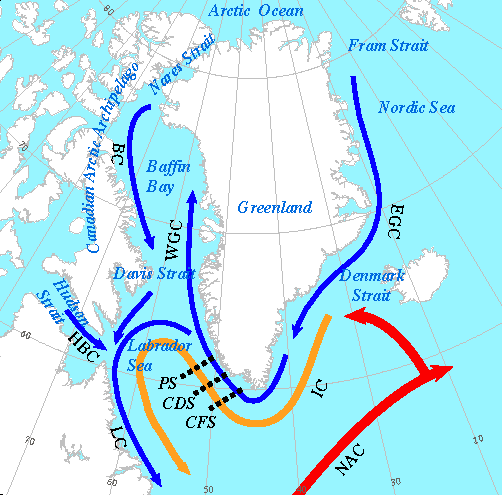
\includegraphics{figs_chpt4/Fig1.pdf}	
	\caption[Study region showing oceanographic sections and major currents around Greenland.]{Study region showing oceanographic sections and major currents around Greenland.  Red and orange arrows indicate Atlantic-origin water, blue arrows indicate Arctic-origin water.   NAC is North Atlantic Current; IC is Irminger Current; EGC is East Greenland Current; WGC is West Greenland Current; BC is Baffin Current; HBC is Hudson’s Bay Current; LC is Labrador Current; CFS is Cape Farewell Section; CDS is Cape Desolation Section; PS is Paamiut Section.  3-D structure of major water masses in the Labrador Sea is shown in Figure \ref{fig:SI4_fig1}.}
	\label{fig:chpt4_fig1}
\end{figure}

\clearpage
\begin{figure}
	\centering
	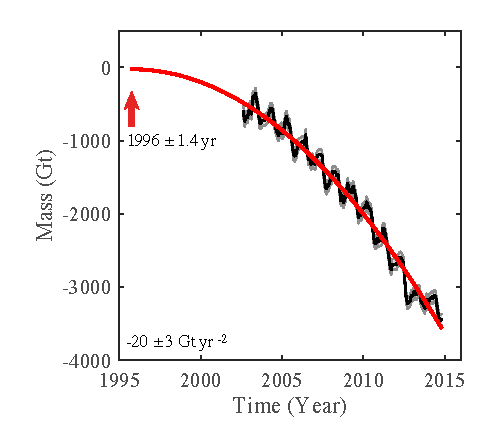
\includegraphics{figs_chpt4/Fig2.pdf}	
	\caption[Mass change of Greenland estimated from GRACE for the period 2002 - 2014.]{Mass change of Greenland estimated from GRACE for the period 2002 - 2014.  Black curve shows data, grey shading indicates monthly uncertainty, and red curve shows the best fitting constant acceleration model.  Onset time of acceleration defined when rate of mass change is zero, in 1996 (red arrow), with mass arbitrarily set to zero.}
	\label{fig:chpt4_fig2}
\end{figure}

\clearpage
\begin{figure}
	\centering
	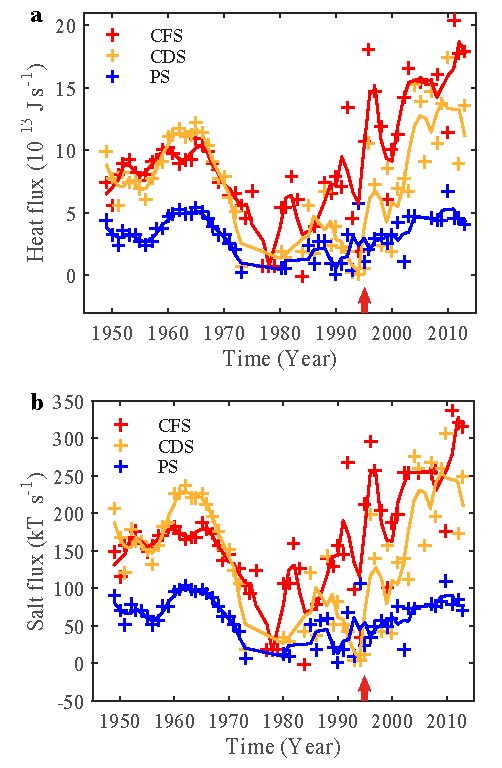
\includegraphics{figs_chpt4/Fig3.pdf}	
	\caption[Heat and salt fluxes of Irminger Water for the period 1949 – 2013.]{Heat and salt fluxes of Irminger Water for the period 1949 – 2013. (a) Heat and (b) salt fluxes of Irminger Water are measured at three sections in southwest Greenland.  Locations of three sections are shown in Figure \ref{fig:chpt4_fig1}.  CFS is Cape Farewell Section; CDS is Cape Desolation Section; PS is Paamiut Section.  Solid line represents a 3-year running average, yearly data shown by plus signs.  Red arrow marks the onset time of accelerated mass loss for Greenland estimated from GRACE (Figure \ref{fig:chpt4_fig2}).}
	\label{fig:chpt4_fig3}
\end{figure}

\clearpage
\begin{figure}
	\centering
	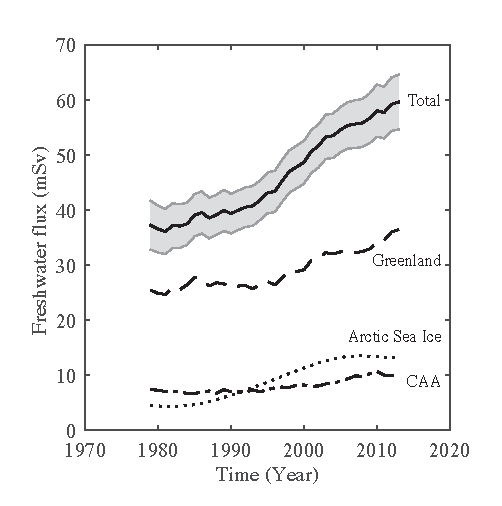
\includegraphics{figs_chpt4/Fig4.pdf}	
	\caption[Freshwater flux from Greenland and CAA and Arctic sea ice for the period 1979 – 2013.]{Freshwater flux from Greenland and CAA and Arctic sea ice for the period 1979 – 2013.  For Arctic sea ice, we plot only changes in flux (see text). The sum of these sources (“Total”) is also plotted.  Grey shading indicates propagated uncertainty (see Appendix B).}
	\label{fig:chpt4_fig4}
\end{figure}

\clearpage
\begin{figure}
	\centering
	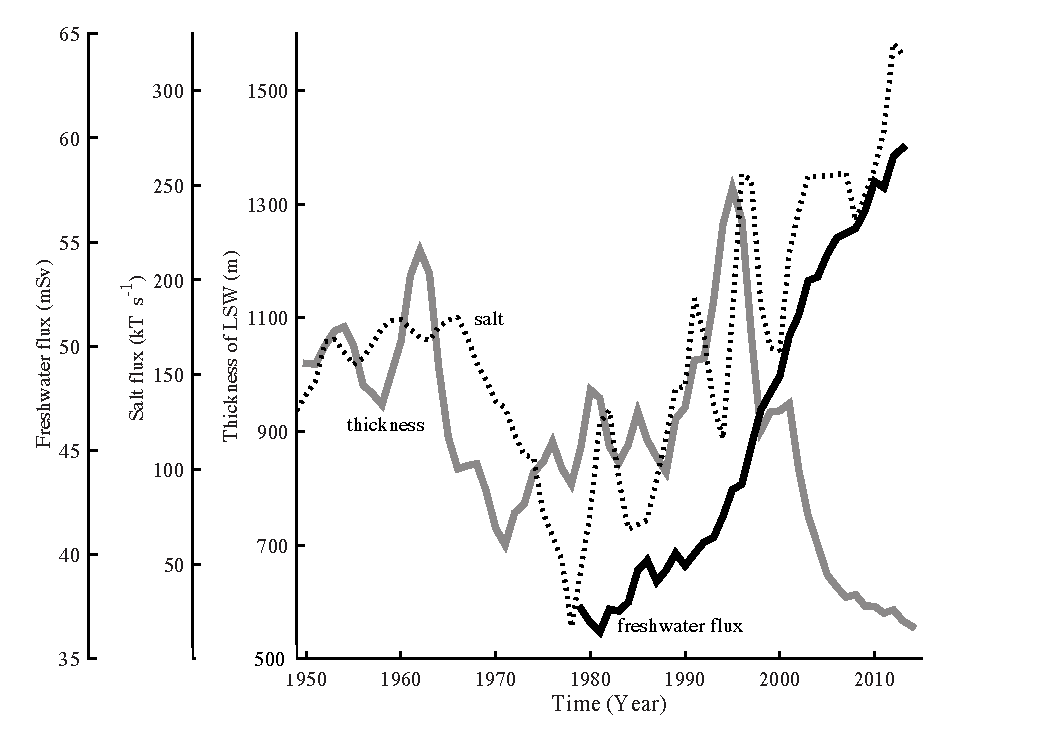
\includegraphics{figs_chpt4/Fig5.pdf}	
	\caption[Thickness of LSW and total freshwater flux and salt flux of Irminger Water.]{Thickness of LSW and total freshwater flux and salt flux of Irminger Water.  Grey solid line indicates thickness of LSW, black solid line indicates total freshwater flux, and dotted line indicates salt flux of Irminger Water.  Thickness and salt flux are smoothed with a 3-year running mean.  Thickness is obtained from the objective analysis of EN4.0.2 dataset from the UK Met Office Hadley Center \cite[]{good2013}. Thickness is averaged over 50 $\textordmasculine$ N - 65 $\textordmasculine$ N and 38 $\textordmasculine$ W – 65 $\textordmasculine$ W.  Expression of salt flux in terms of freshwater flux is shown in Figure \ref{fig:SI4_fig7}.}
	\label{fig:chpt4_fig5}
\end{figure}
\chapter[InSAR Monitoring of Ground Deformation Due to CO$_{2}$ injection at an Enhanced Oil Recovery Site, West Texas]{InSAR Monitoring of Ground Deformation Due to CO$_{2}$ injection at an Enhanced Oil Recovery Site, West Texas \footnote{This chapter has been reprinted from the International Journal of Greenhouse Gas Control with permission as: Yang, Q., Zhao, W. L., Dixon, T. H., Amelung, F., Han, W. S., Li, P., (2015), InSAR Monitoring of Ground Deformation Due to CO$_{2}$ injection at an Enhanced Oil Recovery Site, West Texas, Int. J. Greenhouse Gas Control, 41, 20-28. Copyright 2015 by Elsevier. doi:10.1016/j.ijggc.2015.06.016.}}

% 
% \author[Voytenko and others]{Denis VOYTENKO,$^1$ Alon STERN,$^2$ David M. HOLLAND,$^2$ Timothy H. DIXON,$^1$ Knut CHRISTIANSON,$^2$ Ryan T. WALKER$^{3,4}$}
% 
% \affiliation{%
% $^1$School of Geosciences,
% University of South Florida, Tampa, Florida, USA.\\
% E-mail: qianyang@mail.usf.edu\\
% $^2$Courant Institute of Mathematical Sciences, New York University, New York, New York, USA\\
% $^3$Cryospheric Sciences Laboratory, NASA Goddard Space Flight Center, Greenbelt, Maryland, USA\\
% $^4$Earth System Science Interdisciplinary Center, University of Maryland, College Park, Maryland, USA
% }

\section{Abstract} 
Interferometric Synthetic Aperture Radar (InSAR) measurements have been used to measure ground deformation associated with fluid injection/production at an Enhanced Oil Recovery (EOR) field in Scurry County, West Texas. 100 million tons (Mt) of supercritical CO$_{2}$ have been sequestered here since 1972, of which about half has been sequestered since 2004.  InSAR data show surface uplift up to 10 cm in the field between January 2007 and March 2011.  We evaluated data concerning injection and production of CO$_{2}$, water, oil and hydrocarbon gas from 2004 to 2011 to investigate causes of the observed uplift.  An analytical model is used to calculate reservoir pressure change and surface displacement.  Our simulations show up to 10 MPa pressure buildup in the reservoir over four years of net injection and production.  Surface displacement predictions agree well with the InSAR observations.  Water injection alone cannot explain the 2007 – 2011 surface uplift because the net injected water ($\sim$1~Mt) is negligible compared to the net injected CO$_{2}$ ($\sim$24~Mt).  The predicted total pressure buildup (up to 10 MPa) consists of net CO$_{2}$ injection (up to 12 MPa), net water injection (up to 2 MPa), and oil and gas production (up to -0.4 MPa).  Hence, observed ground uplift was mainly caused by CO$_{2}$ injection.
% \maketitle


\section{Introduction}

An important aspect of large-scale Carbon Capture, Utilization and Storage (CCUS) is the ability to assess the fate of injected CO$_{2}$ and test for leakage.  These so-called Monitoring, Verification and Accounting (MVA) activities typically involve active seismic surveys and down-hole techniques for precise tracking of CO$_{2}$ plume migration, both of which can be expensive.  Since the economic viability of CCUS is impacted by the cost of MVA activities, development of lower cost approaches is desirable.

Injection of CO$_{2}$ or other fluid into a reservoir at depth increases fluid pressure in the reservoir, causing deformation in the overlying strata and inducing surface deformation.  If the pressure change is large enough, the surface deformation may be measurable.  In principle, the measured surface deformation can be inverted to estimate pressure changes at depth and track the CO$_{2}$ plume \cite[e.g.,][]{vasco2008reservoir,vasco2010satellite,rinaldi2013modeling,white2014geomechanical,karegar2015gps}.  Over long periods (decades or centuries), chemical reactions that result in formation of mineral phases will cause pressure and volume reduction and subsidence, and could not be distinguished from migration or leakage with this technique alone.  On the other hand, surface deformation can be measured at relatively low cost, the interpretation is relatively straightforward, and the technique gives useful information in the critical few years immediately following injection.

Enhanced Oil Recovery (EOR) refers to techniques for increasing the amount of oil extracted at depleted or high viscosity oil fields.   CO$_{2}$-Enhanced Oil Recovery (CO$_{2}$-EOR) has been used by the oil and gas industry for over 40 years \cite[]{orr1984use}, but only recently has its potential as a promising method of carbon sequestration been realized and investigated \cite[]{bryant2007geologic}.  Considering the potential of CO$_{2}$-EOR for implementation of large-scale carbon emission reduction \cite[]{metz2005carbon}, it is important to test surface deformation MVA techniques in a CO$_{2}$-EOR field.

Interferometric Synthetic Aperture Radar (InSAR) technique has been successfully used to monitor surface deformation associated with CO$_{2}$ injection at the In Salah field in Algeria \cite[]{mathias2009approximate,morris2011study,shi2012assessment,verdon2013comparison}.  In this paper, we use InSAR to study surface deformation associated with a CO$_{2}$-EOR project in West Texas.  We use an analytical model and historical injection and production data to estimate CO$_{2}$ plume extent and reservoir pressure change constrained by surface deformation observations. The study reveals that ground uplift between January 2007 and March 2011 is mainly caused by CO$_{2}$ injection.   The maximum pressure change due to net injection and production of CO$_{2}$, water, oil and hydrocarbon gas is up to 10 MPa.

\section{Study area description}
The CO$_{2}$-EOR field is located in Scurry County, West Texas (Figure \ref{fig:chpt5_fig1b}).  The reservoir is the southeastern segment of the Horseshoe Atoll play within the Midland basin, one of the largest subsurface limestone reef mounds in the world \cite[]{galloway1983atlas}.  It is a chain of oil fields with the major one being the Kelly-Snyder field.  The producing zones are Pennsylvanian-aged Cisco and Canyon formations, and are comparable to a large class of potential brine storage reservoirs.  Average depth of the producing zones is 2000 m \cite[]{vest1970oil,raines2001review} with average reservoir pressures of 16 MPa and a temperature of 41.5 \textordmasculine C \cite[]{raines66}.  The rock formation porosity (0 – 22.5\%) and permeability (0.1 md – 1760 md) are described in \citet{raines66}.  The reported average porosity and permeability are 9.8\% and 19 mD respectively.  Overlying the producing zone is the Permian-aged Wolfcamp formation, providing a very low permeability seal above the Cisco and Canyon Groups.  The physical properties of the field make it a good candidate for CO$_{2}$-EOR as well as CO$_{2}$ sequestration.

Three production phases occurred in the oil field after it was discovered in 1948 (Figure \ref{fig:chpt5_fig2}).  The primary recovery phase was 1948 – 1951.  During this phase, 5 percent of original oil in place (2.73 billion barrels) was produced by the solution gas driven mechanism, resulting in decline of the original reservoir pressure by 50 percent, from 21.5 MPa to 11.4 MPa \cite[]{dicharry1973evaluation,brummett1976reservoir}.  The secondary recovery phase began in 1954.  During this phase, water-flooding technology was used to produce oil and maintain reservoir pressure.  133 MCM (Million Cubic Meters) of water was injected into the reservoir, and reservoir pressure increased from 11.4 MPa to 16.2 MPa. However, after 17 years of water injection, over 40 percent of original oil in place was still left in the reservoir.

The tertiary/enhanced oil recovery phase started in 1972 \cite[]{crameik1972carbon}.  During this phase, CO$_{2}$ was injected continuously into the reservoir to increase oil production.  From 1972 to 2003, the CO$_{2}$ monthly injection rate was quite stable, with a mean value of 0.28 MCM per month.  The CO$_{2}$ injection rate has increased since 2004.  The mean value of the CO$_{2}$ monthly injection rate in 2004 – 2011 was about six times higher compared to 1972 – 2003.  Although water was also injected into the unit during the third phase, the sequestered water was small compared to the sequestered CO$_{2}$ since injected and produced volumes of water are approximately equal (Figure \ref{fig:chpt5_fig2}).  \citet{raines66} suggested that approximately 55 Mt (70 MCM) of CO$_{2}$ was sequestered in the reservoir from 1972 to 2005 based on a simple mass-balance model.  Our study updates the injection and production data sets to 2011, and suggests that about 100 Mt (128 MCM) of CO$_{2}$ were sequestered in the reservoir from 1972 to 2011, with about 50 percent accumulated from 2004 to 2011. Note that in this paper, all the volume numbers are reported at the reservoir depth with pressure equal to 16 MPa and temperature equal to 41.5 \textordmasculine C.  

\section{Observed ground deformation}
Advanced Land Observing Satellite (ALOS) image data from the Japan Aerospace Exploration Agency (JAXA) are used to monitor surface displacement above the CO$_{2}$-EOR field.  The satellite repeat cycle is 46 days.  Thirteen images were acquired from January 08, 2007 to March 06, 2011 on ascending path 184, frame 640, from which 53 interferograms were generated.  The small Baseline Subset technique \cite[]{berardino2002new} is applied to generate displacement time series.  By using L-band SAR data, the interferometric phase tends to remain coherent even in vegetated areas. To reduce errors caused by phase unwrapping, we use the temporal coherence method \cite[]{pepe2006extension} to mask out pixels with unwrapping error.  SRTM version 4 \cite[]{reuter2007evaluation} 3 arc second DEM data were interpolated to 1 arc second ($\sim$30~m) resolution to remove topographic effects (Figure \ref{fig:chpt5_fig3}). 

A total displacement of up to $\sim$10~cm LOS (line of sight) is detected (Figure \ref{fig:chpt5_fig1b}a).  Note that part of the oil field is not covered by our interferograms.  No active injection or production occurred in this section during the InSAR observation period (discussed in section \ref{section4.3}, Figure \ref{fig:chpt5_fig5}).  Thus, we expect only moderate displacement here associated with nearby injection and production activity.   

Figure \ref{fig:chpt5_fig4}a shows time series of LOS displacement at Snyder, Texas (red star marked in Figure \ref{fig:chpt5_fig1b}).  Increasing LOS displacement is observed from 2007 to 2011 when the cumulative volume of sequestered CO$_{2}$ increased.  From 2007 to 2011, about 31 MCM ($\sim$24~Mt) CO$_{2}$ is stored in the reservoir, significantly larger than the amount of stored water ($\sim$~MCM/1 Mt) (Figure \ref{fig:chpt5_fig4}b), suggesting that the observed surface uplift is mainly caused by CO$_{2}$ injection. 

\section{Simulation}
\subsection{Analytical solution for ground displacement}
An analytical solution for ground displacement associated with injection or withdrawal of fluid at depth may be derived in two steps: a) the approximate solution for reservoir pressure change due to fluid injection \cite[]{mathias2009approximate,mathias2009screening} and production \cite[]{theis1935relation}; and b) the solution for surface deformation due to pressure change in depth estimated in an elastic half space \cite[]{xu2012fluid}.

First, we calculate the reservoir pressure change field due to fluid injection.  Here, the approximate solution of \citet{mathias2009approximate} is adopted to calculate pressure buildup due to injection of CO$_{2}$ in rock formations with large spatial extent.  This solution is derived using the method of matched asymptotic expansions and accounts for two-phase Forchheimer flow (supercritical CO$_{2}$ and water), allowing for slight compressibility of fluid and rock formation.  We also use the solution of Mathias to calculate pressure buildup due to water injection.  Note that the Mathias solution reduces to the \citet{theis1935relation} solution for calculating pressure change due to water injection (single-phase flow) \cite[]{mathias2009approximate}.  We adopt the Theis solution to estimate pressure decline caused by fluid extraction (oil, hydrocarbon gas, water and CO$_{2}$).  \citet{theis1935relation} provides a simplified model to estimate pressure drawdown due to pumping in a homogeneous, isotropic and infinite areal extent reservoir.   We apply the Mathias solution to each injection well and calculate pressure change field caused by CO$_{2}$ injection and water injection respectively.  Note that for wells injecting both CO$_{2}$ and water, we calculate the induced pressure buildup separately regardless of the mixing nature.  As with pressure change due to injection, we apply the Theis equation to calculate pressure change field caused by pumping of each type of fluid (oil, hydro-carbon gas, water and CO$_{2}$) at every individual production well.  In summary, in this step we estimate a pressure change field caused by every single fluid element injected/extracted at an individual well, in preparation for surface displacement calculation in the next step. 

Here we summarize the main formulations of the analytical solution for pressure buildup $P_{inj}(r,t)$  at radial distance $r$ (note that $x$ is dependent on r) and time t due to fluid (CO$_{2}$/water) injection  \cite[]{mathias2009approximate} (equation \ref{eq:chpt5_1}-\ref{eq:chpt5_2}) and the Theis solution for pressure drawdown P\_pro (r,t) due to fluid (CO$_{2}$/water/oil/HC gas) production (eq. \ref{eq:chpt5_3}).

\begin{equation} \label{eq:chpt5_1}
\begin{aligned}
P_{inj}(r,t) & = P_{0}\{\dfrac{1}{2\gamma}Ei(\dfrac{\alpha x}{4\gamma})+\dfrac{1}{2\gamma}(\ln(\dfrac{\alpha x}{4\gamma})+0.5772)\} \\
& + P_{0}
\left\lbrace
  \begin{array}{lr}
  -\dfrac{1}{2}\ln(\dfrac{x}{2\gamma})-1 + \dfrac{1}{\gamma} - \dfrac{1}{\gamma}(\ln(\dfrac{\alpha x}{2\gamma^2})+0.5772) & x\leq 2\gamma \\
  -(\dfrac{x}{2\gamma})^{0.5} + \dfrac{1}{\gamma} - \dfrac{1}{2\gamma}(\ln(\dfrac{\alpha x}{2\gamma^2})+0.5772) & 2\gamma \leq x\leq \dfrac{2}{\gamma} \\
  -\dfrac{1}{2\gamma}(\ln(\dfrac{\alpha x}{4\gamma})+0.5772) & x\geq \dfrac{2}{\gamma} 
  \end{array}
\right\rbrace 
\end{aligned} 
\end{equation} 

where:
$Ei$ is the exponential integral operator.
\begin{equation} \label{eq:chpt5_2}
\begin{aligned}
& P_{0} = \dfrac{Q_m\mu_f}{2\pi H \rho_{f} \kappa} \\
& \gamma = \dfrac{\mu_{f}}{\mu_{brine}} \\
& x = \dfrac{(r/r_w)^2}{tQ_m/(2\pi\omega H(r_w)^2 \rho_f)} \\
& \alpha = \dfrac{Q_m \mu_f (c_{rock}+c_{brine})}{2\pi H \kappa}
\end{aligned}
\end{equation}
where: 
$r$ is the radial distance to injection well ($m$); $r_w$ is the injector well radius, and we use $r_w = 0.1\ m$ for our calculation; $\rho_f$ is the density of injected fluid ($kg/m^3$); $\mu_f$ is the viscosity of injected fluid ($Pa\cdot s$); $Q_m$ is the mass injection rate ($kg/s$); $t$ is the injection time ($s$); $c_{rock}$ is the formation compressibility ($Pa^{-1}$); $\kappa$ is the formation permeability ($m^2$); $\mu_{brine}$ is the brine compressibility ($Pa^{-1}$); $H$ is the formation thickness ($m$). 

\begin{equation} \label{eq:chpt5_3}
\begin{aligned}
P_{pro}(r,t) = -\dfrac{Q_{\nu} \mu_{f}}{4 \pi \kappa H}
				Ei(-\dfrac{\mu_f(\phi c_f + c_{rock}) r^2}{4 \kappa t})
\end{aligned}
\end{equation}
where:
$Q_{\nu}$ is the volume injection rate ($m^3/s$); $\mu_f$ is the viscosity of produced fluid ($Pa\cdot s$); $c_f$ is the compressibility of produced fluid ($Pa^{-1}$);  $\phi$ is the formation porosity; other parameters are the same as in equation \ref{eq:chpt5_1} and equation \ref{eq:chpt5_2}.   Values of those parameters used in computing the pressure change are listed in Table \ref{tab:table1} - \ref{tab:table2}.  

Second, given the calculated fluid pressure field, we then calculate induced surface displacement.  \citet[]{xu2012fluid} provide an analytical elastic solution for displacement in a half space forced by an arbitrary pressure distribution in the reservoir.  Since the pressure caused by injection/production at individual well can be approximated as radial distribution, we first use Xu's solution to estimate surface displacement centered at each well according to the radial distributed pressure field of that well.  Then, surface displacement of each well is linearly summed up to get the total surface displacement field due to all injection and production activities.  

The main formulations of the analytical solution for vertical displacement $u_{z}(r)$ and horizontal displacement $u_{r}(r)$ at the radial distance r at the free surface results from the cumulative contribution of all the rings of dilation at radius $r_{0}$ and depth $z'$ \cite[]]{xu2012fluid}.

\begin{equation} \label{eq:chpt5_4}
\begin{aligned}
& u_{z}(r)=-\frac{2(1+\nu)(1-2\nu)}{\pi E} \iiint \limits_{0 0 Z_1}^{\ \ \ \infty \pi Z_2} 
\frac{p(r_{0},t) z'}{(z'^{2} + r^2 + r_{0}^2 - 2rr_{0}cos\varphi)^{1.5}} r_{0} dz' d\varphi dr_{0} \\
& u_{r}(r)= \frac{2(1+\nu)(1-2\nu)}{\pi E} \iiint \limits_{0 0 Z_1}^{\ \ \ \infty \pi Z_2} 
\frac{p(r_{0},t) (r-r_{0}cos\varphi)}{\rho'^3 (z'^{2} + r^2 + r_{0}^2 - 2rr_{0}cos\varphi)^{1.5}} r_{0} dz' d\varphi dr_{0}
\end{aligned}
\end{equation}

where:
$\nu$ is the Poisson’s ratio; E is the Young’s modulus (GPa); $p(r_0,t)$  is the pressure change ($Pa$) at radial distance $r_0$ and time $t$,  $\phi$ is the difference of azimuthal angle between surface point and the dilation center; $z_1$ is the depth of reservoir lower bound ($m$) and $z_2$ is the depth of reservoir upper bound ($m$). 

Each of these solutions has been validated through numerical simulations \cite[]{xu2012fluid,mathias2009approximate} or comparison with in situ observation \cite[]{theis1935relation}. However, the analytical model used in our paper has its limitations relating to the complexity of subsurface structure and deformation processes.  But the simple analytical allows us to estimate large-scale pressure change and surface displacement by considering the realistic injection and production history for hundreds of operation wells.  The calculation time is fast compared to more complex models, and as we shall show, provides an adequate fit to our data. 

\subsection{Input parameters of the analytical simulations}
The depth and thickness of the reservoir are irregular \cite[]{han2010evaluation}.  In our model, we use an average thickness of 200 m, ranging from depth 2000 m to 2200 m, based on the depths of injection wells provided by Railroad Commission of Texas (RRC) and personal communication with the operator of the field.  The average porosity (9.8\%) and permeability (19 mD) reported by \citet{raines66} were measured from a core-flooding test, which typically does not include reservoir scale imperfections such as fractures and other forms of secondary porosity. Obviously, the reservoir is very heterogeneous \cite[]{han2010evaluation} but our analytical solution only requires mean porosity and permeability values.  To better represent its variation, we choose three levels of porosity and permeability (low, medium and high), and predict three corresponding sets of pressure change and surface displacement.  We utilize the relationship between porosity and permeability for the Canyon formation (the third sequence) given by \citet{lucia2004permeability} to calculate permeability based on three-levels of porosity (Table \ref{tab:table1}).  Rock formation (limestone) compressibility is obtained from \citet{newman1973pore}.  These and other properties of the reservoir formation are summarized in Table \ref{tab:table1}.  We further assume that the extracted hydrocarbon gas is purely methane, and that the salt concentration of injected water is 0.15 kg/l.

Fluid properties (CO$_{2}$, water, methane and oil) at reservoir pressure (16 MPa) and temperature (41.5 \textordmasculine C) are summarized in Table \ref{tab:table2}.  Properties of supercritical CO$_{2}$ and methane are obtained from the NIST fluid properties website (http://webbook.nist.gov/chemistry/fluid/).  Properties of salt water are derived based on the empirical correlations with pressure, temperature and salt concentration shown in \citet{mathias2009screening}.  Density and viscosity of the produced oil are obtained from \citet{vest1970oil}.  Oil compressibility is obtained from \citet{satter2008practical}.

Two geomechanical parameters, Young’s modulus and Poisson’s ratio, are needed for surface displacement calculation.  However, there are no publicly available data for these two geomechanical properties for the overlaying Walfcamp shale.  Since surface displacement is less sensitive to Poisson’s ratio, a common result in many Earth deformation problems \cite[e.g.,][]{bevis2005seasonal}, we set the value of Poisson’s ratio to 0.25, and then forward model to estimate the value of Young’s modulus that best fits the surface displacement observed by InSAR. We selected a profile across the significant inflation area for comparison between model simulation and InSAR observation (Figure \ref{fig:chpt5_fig1b}).  Grid search ranges are 1 – 50 aa with search increments of 1 GPa.  Goodness of fit is assessed using the standard chi-square statistic.

\subsection{Injection and production data during 2004 - 2011} \label{section4.3}
Monthly injection and production rates during 2004 to 2011 at individual wells in the field were provided by the field operator. Information concerning locations and depths of individual wells is provided by the RRC.  Both CO$_{2}$ and water were injected into the reservoir from 2004 to 2011 (Figure \ref{fig:chpt5_fig2}).  In detail, 409 wells injected CO$_{2}$; 217 wells injected water and 603 wells extracted oil and HC gas.  In this field, injected CO$_{2}$ is often mixed with water, and extracted oil and HC gas are often mixed with CO$_{2}$ and water.  Location of active injection and production wells during 2004 - 2011 is shown in Figure \ref{fig:chpt5_fig5}.  

To reduce the computation we divide the field into grids of 500 m width (Fig. \ref{fig:chpt5_fig6}). We then approximate the injection/production history by placing a virtual well at the center of each grid.  For CO$_{2}$ and water, we calculate the mean injection/extraction rate by adding the net fluid injection and extraction for that grid respectively.  For oil and HC gas, the production rate is set equal to the net fluid extracted for that grid. 

To compare with InSAR observations, we should predict surface displacement from January 2007 to March 2011.  However, pressure change due to constant rate injection/production is not linear with time: fluid pressure changes significantly in the first few months and then slows down \cite[]{rohmer2012applicability}.  Thus, for a well being operated before 2007, pressure change during 2007 to 2011 cannot be simply calculated by just using data from January 2007 to March 2011.  To address this problem, we check the injection/production history of every well to see if there is any operation before 2007.  If there is, we calculate pressure changes during two periods for that well: one period from the beginning of operation to March 2011 and second period from the beginning of operation to December 2006. We then subtract the pressure change during the second phase from the pressure change during the first phase to derive pressure change between January 2007 and March 2011 (the period of InSAR observations).   If there is no operation prior to 2007, pressure change is calculated using data from January 2007 to March 2011.  It is worth noting that fluid production and injection in the field started in 1948 and 1954 respectively, and we only have injection/production data for each well from 2004. Thus, in our simulation, the operational beginning of each well is not earlier than 2004.  

\section{Simulation results}
Figure \ref{fig:chpt5_fig7} shows the simulated changes in reservoir pressure due to different fluid injection/extraction rates for three assumed values of rock formation porosity and permeability.  The local maxima and minima patterns are similar for the different values of porosity and permeability.  Calculated pressure change in the reservoir decreases for higher values of porosity and permeability.  Net CO$_{2}$ injection/production significantly affects reservoir pressure.  Since volumes of water injection and production are approximately the same (Figure \ref{fig:chpt5_fig2}, Figure \ref{fig:chpt5_fig4}b), pressure changes due to net water injection are negligible compared to those caused by net CO$_{2}$ injection, indicating that surface uplift observed by InSAR is dominated by CO$_{2}$ injection. Net water injection/production causes pressure buildup/drawdown in different areas of the field.  Net oil and hydrocarbon gas production generally causes pressure drawdown in the field.  In summary, pressure changes due to CO$_{2}$ injection and production are much higher than that caused by water injection/production and oil/hydrocarbon gas production.

Figure \ref{fig:chpt5_fig8} shows the simulated total pressure buildup due to all fluid injection and oil/hydrocarbon gas production production for three assumed values of porosity and permeability. The low value of porosity and permeability condition yields pressure buildup up to 10 MPa, while the high value yields up to 2 MPa pressure buildup. Maximum pressure buildup is more spread out for the high porosity and permeability values.

Based on the simulated pressure change field, a grid search method was used to estimate the value of Young’s modulus that best fits the InSAR observations along the profile marked in Figure \ref{fig:chpt5_fig1b}.   To compare with InSAR LOS displacement, we convert the predicted surface displacement to LOS displacement using satellite azimuth and incidence information.  Figure \ref{fig:chpt5_fig9} shows goodness of fit versus Young’s modulus at three levels of pressure change.  The best-fit values for Young’s moduli are listed in Table \ref{tab:table3}.  Predicted LOS displacements using the best-fit Young’s modulus at the three levels of pressure change are compared to the InSAR data along the profile (Figure \ref{fig:chpt5_fig10}).  All three predictions agree well with InSAR observations along the profile.  The high-pressure condition provides the smallest misfit between model prediction and observation, but the difference with the other models is small.  The low and medium pressure conditions also provide a good fit between model prediction and observation.  However, the best-fit Young’s moduli derived from the low and medium pressure conditions (6 GPa  and 10 GPa) are quite small compared to the best-fit Young’s modulus derived from the high-pressure condition (18 GPa), and are on the low side of plausible crustal values.   A similar deformation study in south Texas \cite[]{karegar2015gps} where pressure data were available for calibration gave a best estimate of average Young’s modulus of 55 GPa +80/-20 GPa; at 95\% confidence, the minimum estimate obtained in that study was 15 GPa, similar to our high estimate.  We therefore take the estimate of 18 GPa as the most plausible value for Young’s modulus and the corresponding estimate of the high-pressure buildup condition (up to 10 MPa) as the best pressure change estimate.

We then predict 2D LOS displacement fields for the three models of pressure change respectively using the best-fit Young’s modulus derived from the profile fitting analysis.  Simulated 2D LOS displacement at the high-pressure change condition and the residual between InSAR observation and model prediction are shown in Figure \ref{fig:chpt5_fig11}.  Our simulation is able to match most of the uplift signal observed by InSAR.  However, up to 4 cm of residual uplift remains.  The residuals likely reflect a combination of atmospheric and reservoir heterogeneity.  The former reflects deviations from the assumption used in our data analysis that atmospheric properties are laterally uniform.  The latter reflects deviations from the assumption used in our modeling that the rheological properties of the reservoir are vertically and horizontally uniform. 

\section{Discussion}
We modeled a reservoir as a simplified body with uniform properties.  In fact, it almost certainly has significant spatial variation in porosity, permeability and elastic properties.  We have also ignored inter-well pressure interaction when simulating reservoir pressure change.  Despite these simplifications, we are able to obtain good fits to the surface deformation data and obtain useful information on the reservoir.  This reflects the fact that the free surface is 2000 m above the reservoir, hence the effects of reservoir heterogeneity and inter-well pressure interactions on surface deformation are relatively small.  In effect, the intervening crustal material acts like a low pass filter, attenuating short wavelength strain effects associated with spatial complexities of the reservoir and the injected fluid.  

The relatively large uncertainty in our estimate of Young’s modulus reflects the weak resolving power of surface deformation data for this parameter.  Independent determination of Young’s modulus from down-hole measurements, 3-D seismic surveys, or laboratory experiments on well bore samples would allow a more quantitative link between surface deformation and reservoir pressure change.

\citet{gan2013gas} suggested that increasing earthquakes in the Cogdell field, north of our study area, during 2006 – 2011 were likely triggered by CO$_{2}$ injection.  However, our study area, which has also experienced significant fluid injection over the same time period, has not experienced a significant increase in seismicity.  Meanwhile, InSAR data show no surface uplift in the Cogdell field, while measurable uplift is observed in our study area.  The different seismic and deformation responses to fluid injection between these two fields may reflect differences in regional subsurface structures.  Our study area has been mapped as a single large reef mound, but structures in the Cogdell field show more spatial variation \cite[]{vest1970oil}. The Cogdell limestone may have experienced more intense weathering and karsting compared to our study area \cite[]{reid1991cogdell}, potentially creating more heterogeneous structures, and potential faults and fractures.  The recent earthquakes suggest the presence of faults in the Cogdell field.   The absence of mapped faults and earthquake activity in our study area suggests no active faulting.  Perhaps triggered earthquakes occur when injected gas or fluid reaches suitably orientated pre-existing faults, reducing the resolved normal stress and hence the effective friction, and promoting seismic slip on pre-existing faults.  

\section{Conclusions}
We evaluated injection and production data for CO$_{2}$, water, oil and hydrocarbon gas at individual wells in a CO$_{2}$-EOR field between 2004 and 2011. Approximately 50 Mt of CO$_{2}$ were sequestered between 2004 and 2011, equal to the total sequestered CO$_{2}$ between 1972 and 2003.  InSAR data observe up to 10 cm line of sight displacement between January 2007 and March 2011 in this field.  Water injection alone cannot explain surface uplift between January 2007 and March 2011 because net injected water ($\sim$1~Mt) is negligible during this period.  However, significant amounts of CO$_{2}$ ($\sim$24~Mt) were injected into the reservoir, contributing to observed surface uplift.  An analytical simulation relating reservoir pressure and surface displacement using realistic injection and production data from individual wells predicts up to 10 MPa pressure buildup due to net fluid injection and production in 2007- 2011, using assumed average values of porosity and permeability.  With better information on the mechanical properties of the reservoir, InSAR data could directly estimate reservoir pressure changes with time.  

\section{Acknowledgements}
We thank the field operator for providing historical injection and production data. We also thank the Railroad Commission of Texas for providing information on the location and depth of individual wells in our study area. This research was supported by DOE grant DE-FE0001580. We thank Karen Kluger for support and advice throughout our project and two anonymous reviewers for thoughtful comments.  

\section{References}
\bibliographystyle{apalike}  
\bibliography{chpt5_ref}


\clearpage
\begin{table}[h!]
	\begin{center}
		\begin{threeparttable}
			\caption{Reservoir homogeneous properties used for pressure change calculation.}
			\label{tab:table1}
			\begin{tabular}{cccccc}
				\midrule
				Reservoir Property & Symbol & Value & & & Unit\\
				\midrule
				Porosity & $\varphi$ & 0.2(L) & 0.25(M) & 0.3(H) & \%\\
				Permeability & $\kappa$ & 17(L) & 57(M) & 152(M) & mD\\
				Initial pressure & \textit{P$_{0}$} & 16 & & & MPa\\
				Temperature & \textit{T} & 41.5 & & & $^{\circ}$C\\
				Depth (reservoir upper bound) & \textit{Z$_{1}$} & -2000 & & & m\\
				Depth (reservoir lower bound) & \textit{Z$_{2}$} & -2200 & & & m\\
				Thickness & \textit{H} & 200 & & & m\\
				Formation compressibility & \textit{C$_{rock}$} & 5.3E-10 & & & 1/Pa\\
				\midrule
			\end{tabular}
			\begin{tablenotes}
				\small
				\item Note: \textit{L}, \textit{M} and \textit{H} represent low level, medium level and high level of porosity and permeability, respectively.
			\end{tablenotes}
		\end{threeparttable}
	\end{center}
\end{table}

\clearpage
\begin{table}[h!]
	\begin{center}
		\caption{Fluid properties at depth (16MPa,41.5 $^{\circ}$C).}
		\label{tab:table2}
		\begin{tabular}{ccccccc}
			\midrule
			Fluid property & Symbol &\multicolumn{4}{c}{Value} & Unit \\
			\cmidrule(l){3-6}
			&& Brine & CO2 & Methane & Oil &\\
			\midrule
			Density & $\rho$ & 1105 & 784 & 115 & 818 & kg/m$^{3}$\\
			Viscosity & $\mu$ & 9.41E-04 & 6.85E-05 & 1.67E-05 & 3.75E-04 & Pa$\cdot$s\\
			Compressibility & C & 3.40E-10 & 2.10E-08 & 5.43E-08 & 2.17E-09 & 1/Pa\\
			\midrule
		\end{tabular}
	\end{center}
\end{table}

\clearpage
\begin{table}[h!]
	\begin{center}
		\begin{threeparttable}
		\caption{Highest pressure buildup and best-fit Young's modulus at three levels of porosity and permeability.}
		\label{tab:table3}
		\begin{tabular}{cccc}
			\midrule
			Level of porosity and permeability & Highest $\triangle$\textit{P} (MPa) & Best-fit \textit{E} (GPa) & $\chi$$^{2}$\\
			\midrule
			Low & 10.32 & 18 & 0.78\\
			Medium & 4.32 & 10 & 0.80\\
			High & 2.10 & 6 & 0.83\\
			\midrule						
		\end{tabular}
		\begin{tablenotes}
			\small
			\item Note: \textit{E} represents Young's modulus. $\triangle$\textit{P} represents calculated pressure change. $\chi$$^{2}$ represents normalized chi square value.
		\end{tablenotes}
		\end{threeparttable}
	\end{center}
\end{table}

\clearpage
\begin{figure}
\centering
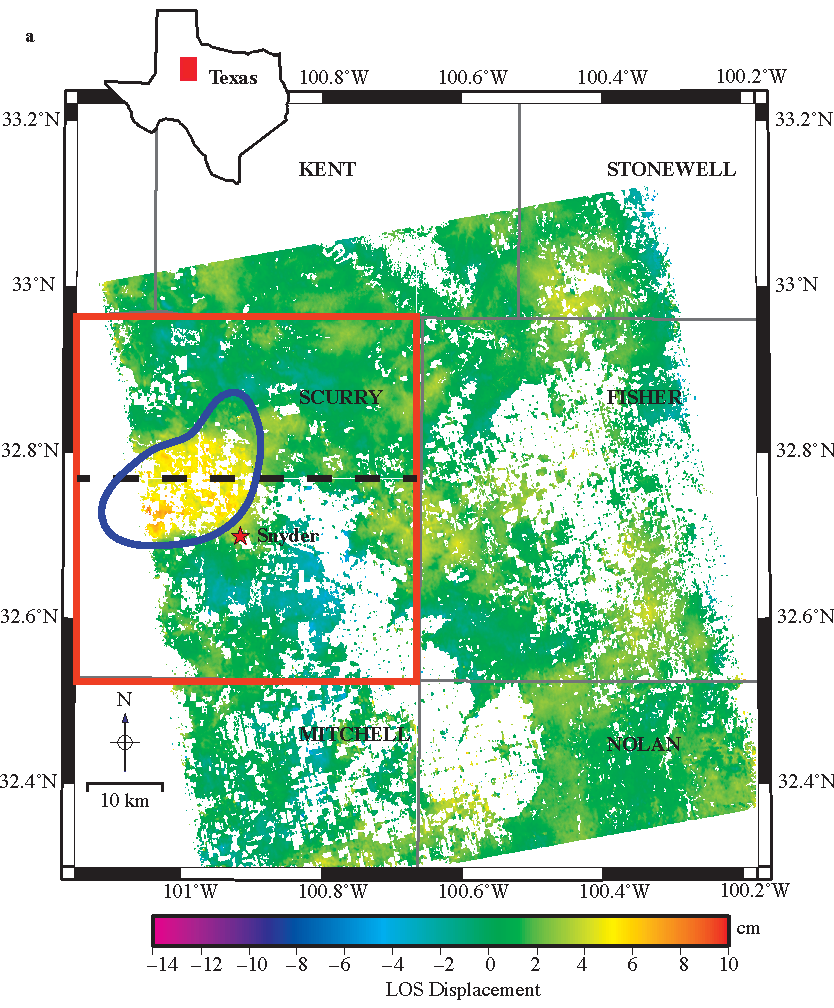
\includegraphics{figs_paper3/Fig1a.pdf}
\label{fig:chpt5_fig1a}
\end{figure}

\clearpage
\begin{figure}
\centering
\includegraphics{figs_paper3/Fig1b.pdf}	
\caption[(a) Total LOS (line of sight) displacement from from January. 08, 2007 to March. 06, 2011. (b) A SAR intensity image of the study area.]{(a) Total LOS (line of sight) displacement from from January. 08, 2007 to March. 06, 2011. (b) A SAR intensity image of the study area.  Red star represents location of the town of Snyder, Texas.  Light grey lines are county boundaries and county names are labeled.  Red lines are the boundaries of our study area, Scurry County.  Blue line is the approximate boundary of the oil field in the study area.  Black dashed line represents location of a profile for surface displacement modeling in the following sections.}
\label{fig:chpt5_fig1b}
\end{figure}

\clearpage
\begin{figure}
	\centering
	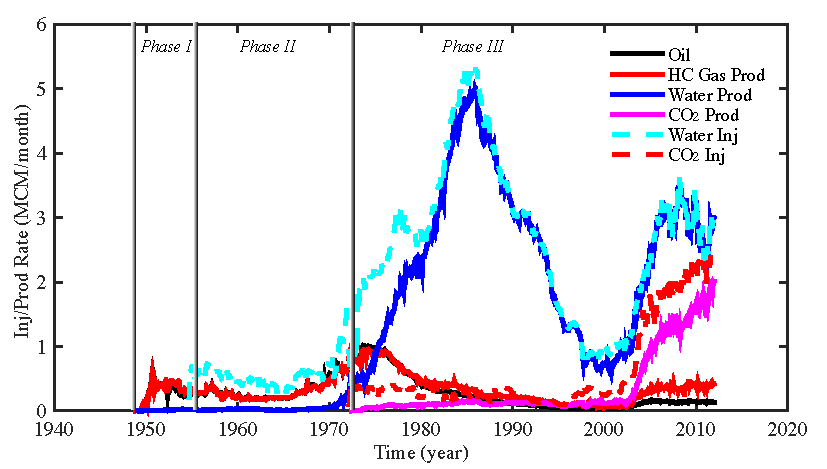
\includegraphics{figs_paper3/Fig2.pdf}	
	\caption[Injection and production history of the study site.]{Injection and production history of the study site.  Phase I is the primary recovery phase.  Phase II is the secondary recovery phase.  Phase III is the tertiary/enhanced oil recovery phases.  Volumes of fluid injection and production are reported at 16 MPa, 41.5 \textordmasculine C (pressure and temperature at reservoir depth). HC is hydrocarbon.}
	\label{fig:chpt5_fig2}
\end{figure}

\clearpage
\begin{figure}
	\centering
	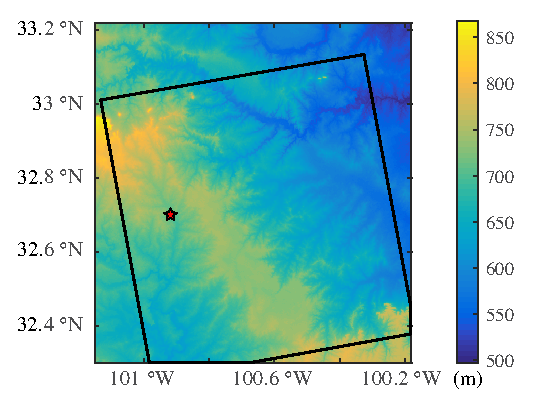
\includegraphics{figs_paper3/Fig3.eps}	
	\caption[DEM of our study area.]{DEM of our study area.  Black lines are the boundaries of the area covered by the interferogram.  Red star represents location of the town Snyder, Texas.}
	\label{fig:chpt5_fig3}
\end{figure}

\clearpage
\begin{figure}
	\centering
	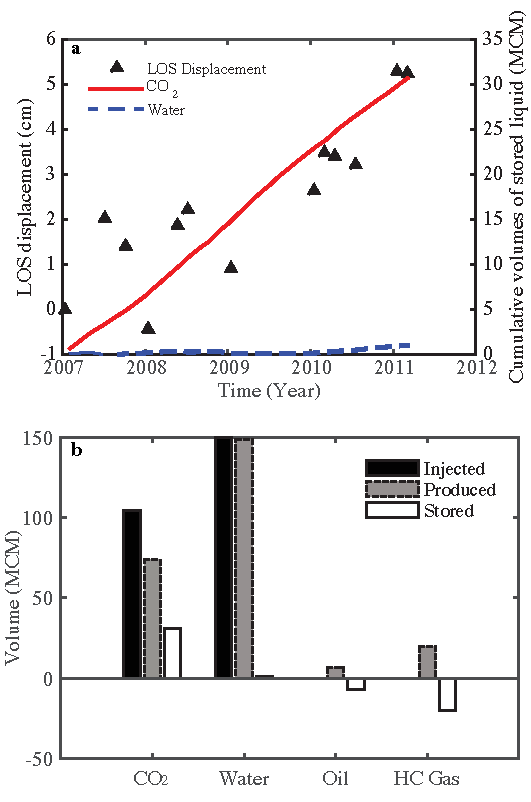
\includegraphics{figs_paper3/Fig4.pdf}	
	\caption[(a) Comparison between Line of Sight (LOS) displacement at Snyder (red star marked in Figure \ref{fig:chpt5_fig1b}) and cumulative volumes of stored (injection minus production) CO$_{2}$ and water in the field from January 2007 to March 2011.  (b) The total volumes of injected/produced/stored CO$_{2}$, water, oil and HC gas in the field from January 2007 – March 2011.]{(a) Comparison between Line of Sight (LOS) displacement at Snyder (red star marked in Figure \ref{fig:chpt5_fig1b}) and cumulative volumes of stored (injection minus production) CO$_{2}$ and water in the field from January 2007 to March 2011.  (b) The total volumes of injected/produced/stored CO$_{2}$, water, oil and HC gas in the field from January 2007 – March 2011.  Volumes of fluid injection and production are reported at 16 MPa, 41.5 \textordmasculine C.}
	\label{fig:chpt5_fig4}
\end{figure}

\clearpage
\begin{figure}
	\centering
	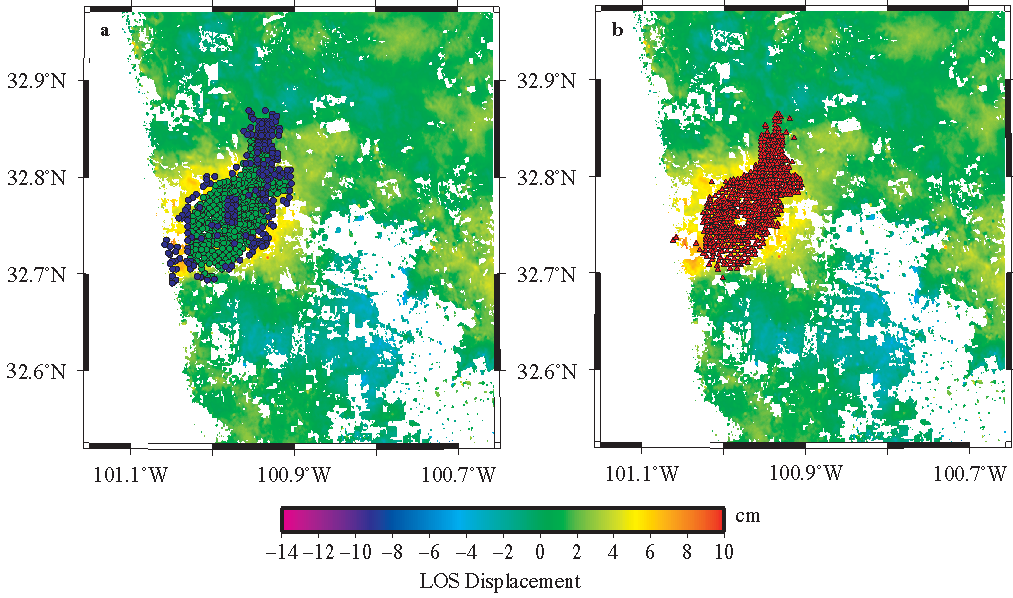
\includegraphics[width=\textwidth]{figs_paper3/Fig5.pdf}	
	\caption{Map of study area, showing total LOS displacement from January 08, 2007 to March. 06, 2011, (a) wells injecting CO$_{2}$ (green circle) and water (blue circle), and (b) well producing CO$_{2}$, water, Oil and HC gas (red triangle).}
	\label{fig:chpt5_fig5}
\end{figure}

\clearpage
\begin{figure}
	\centering
	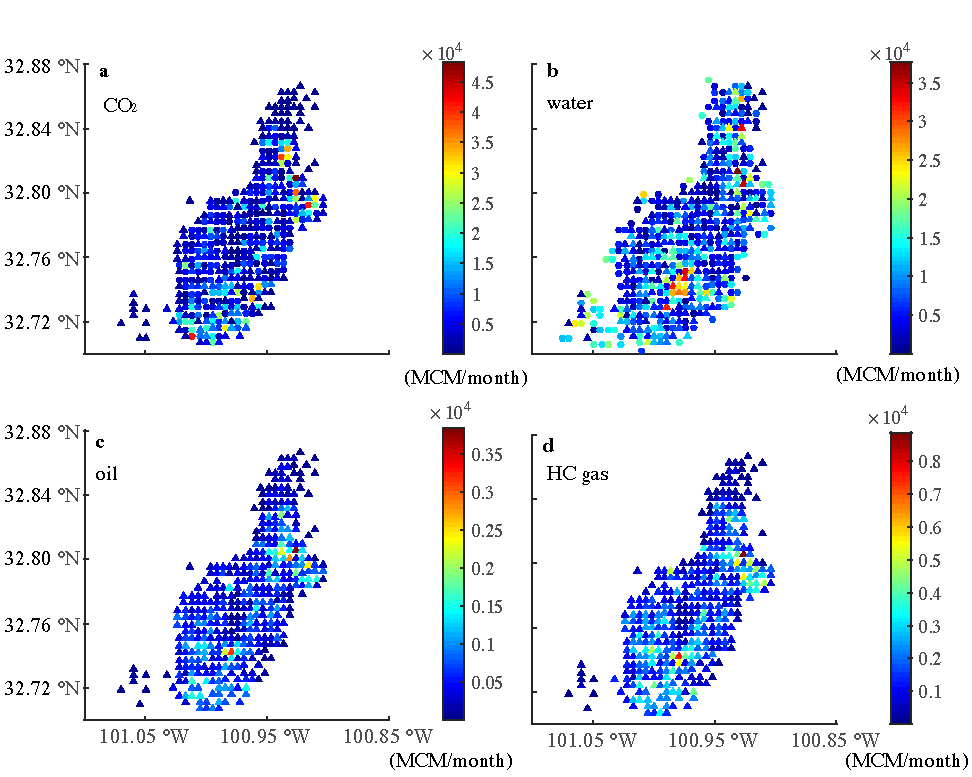
\includegraphics{figs_paper3/Fig6.pdf}	
	\caption[Location of virtual wells for each type fluid and the average monthly injection/production rate for each virtual well.]{Location of virtual wells for each type fluid and the average monthly injection/production rate for each virtual well.  Circles represent injection wells and triangles represent production wells.  Volumes of fluid injection and production are reported at 16 MPa, 41.5 \textordmasculine C.}
	\label{fig:chpt5_fig6}
\end{figure}

\clearpage
\begin{figure}
	\centering
	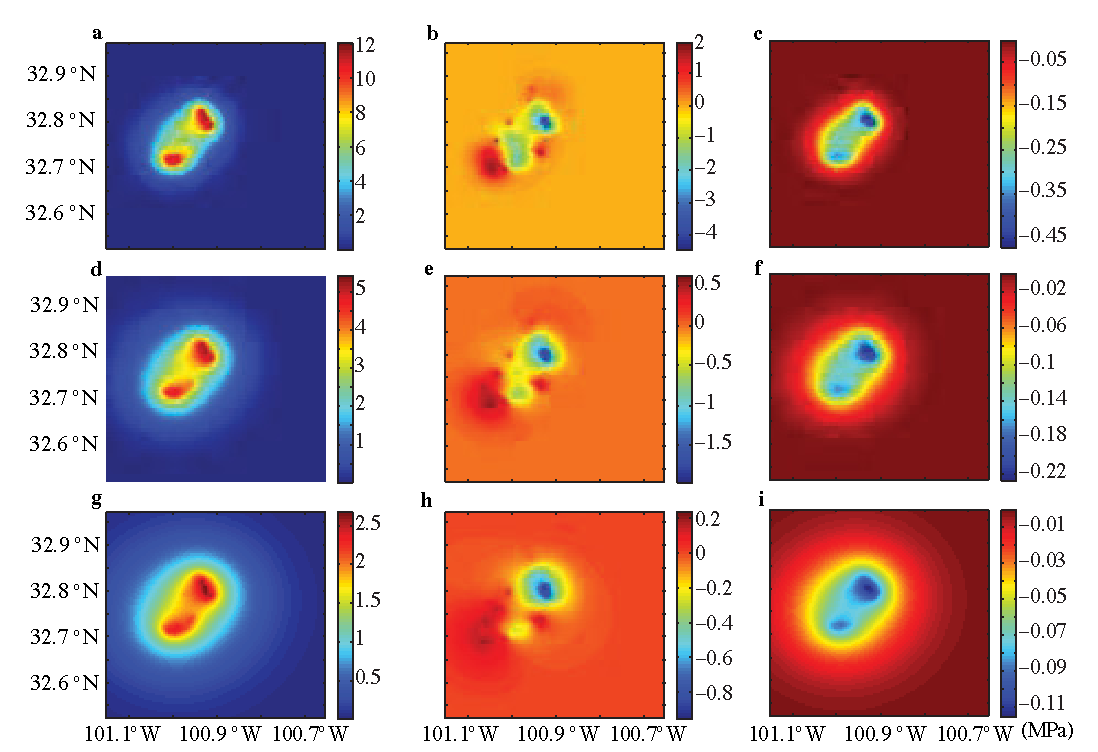
\includegraphics[width=\textwidth]{figs_paper3/Fig7.pdf}	
	\caption[Calculated pressure change due to fluid injection and production at three levels of porosity and permeability.]{Calculated pressure change due to fluid injection and production at three levels of porosity and permeability. (a-c: low porosity/permeability; d-f: medium porosity/permeability; g-i: high porosity and permeability).  a,d and g are calculated pressure buildup due to net CO$_{2}$ injection.  b, e and h are derived from net water injection.  c, f and I are derived from oil and HC gas production}
	\label{fig:chpt5_fig7}
\end{figure}

\clearpage
\begin{figure}
	\centering
	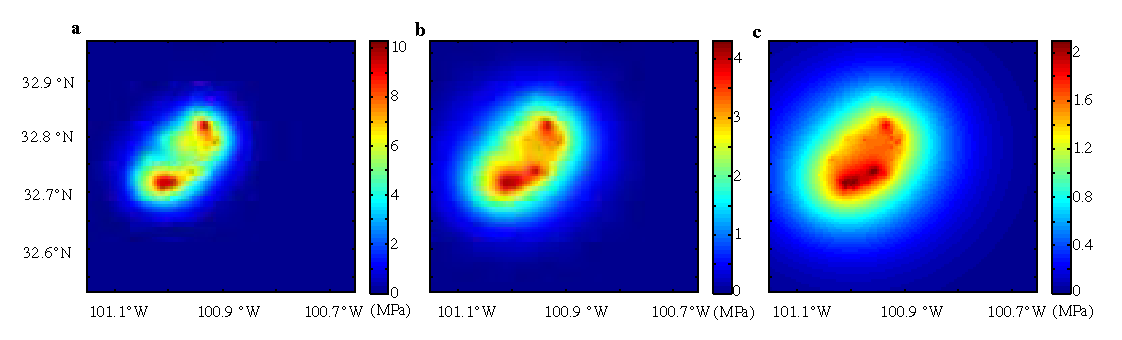
\includegraphics[width=\textwidth]{figs_paper3/Fig8.pdf}	
	\caption[Calculated pressure change due to all injection and production activities at three levels of porosity and permeability.]{Calculated pressure change due to all injection and production activities at three levels of porosity and permeability. (a) low porosity/permeability level; (b) medium porosity/permeability level; (c) high porosity and permeability level.}
	\label{fig:chpt5_fig8}
\end{figure}

\clearpage
\begin{figure}
	\centering
	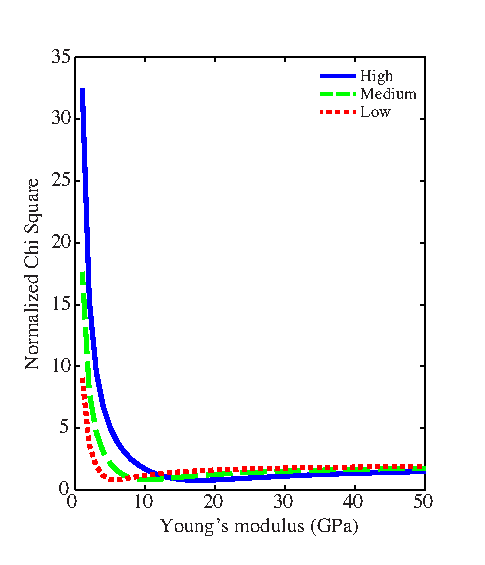
\includegraphics{figs_paper3/Fig9.eps}	
	\caption[Goodness of fit versus Young’s modulus at three levels of pressure change conditions.]{Goodness of fit versus Young’s modulus at three levels of pressure change conditions.  Simulated LOS displacements are fitted to LOS displacement observation along the profile shown in Figure \ref{fig:chpt5_fig1b}.  Note that the minimum value of Young’s modulus is well constrained, but the upper bound value is not.}
	\label{fig:chpt5_fig9}
\end{figure}

\clearpage
\begin{figure}
	\centering
	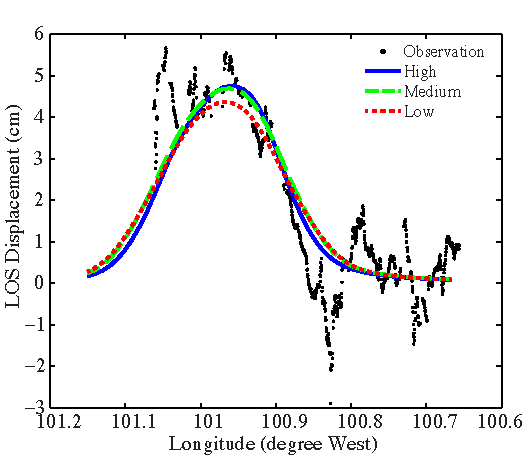
\includegraphics{figs_paper3/Fig10.pdf}	
	\caption{Simulated LOS displacement at three levels of pressure change conditions versus InSAR observation along the profile shown in Figure \ref{fig:chpt5_fig1b}.}
	\label{fig:chpt5_fig10}
\end{figure}

\clearpage
\begin{figure}
	\centering
	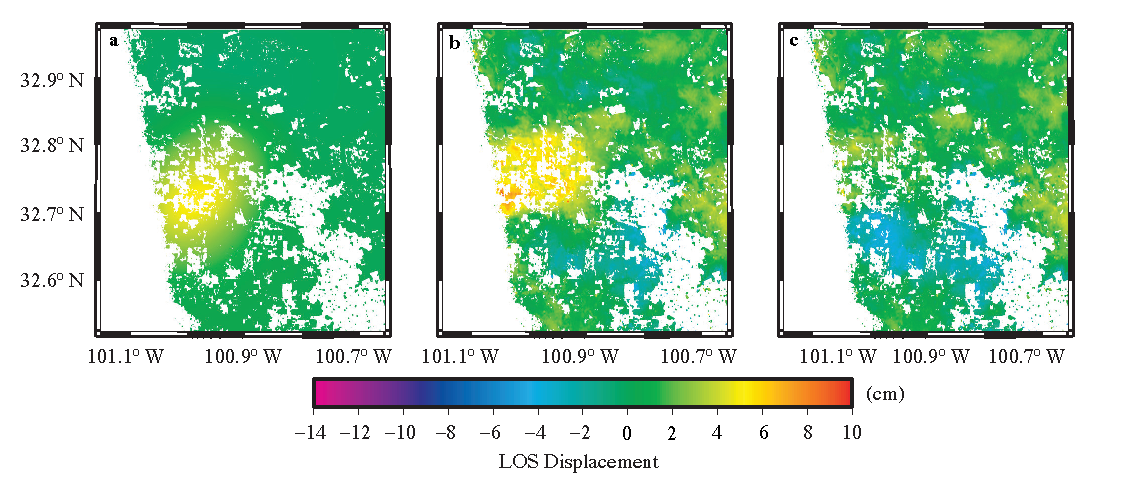
\includegraphics[width=\textwidth]{figs_paper3/Fig11.pdf}	
	\caption[Comparison between simulated LOS displacements and InSAR observation for the entire study area.]{Comparison between simulated LOS displacements and InSAR observation for the entire study area.  Surface displacements were derived from high-pressure change condition.  (a) Simulated LOS displacements; (b) InSAR observation; (c) residual.}
	\label{fig:chpt5_fig11}
\end{figure}
% \end{document}

\chapter{Conclusions and Future Work}
\section{Conclusions}
This dissertation presents three studies that use satellite geodesy to study environmental and global change.  The main conclusions from these studies are described in Chapters Three, Four and Five and are summarized here. 

Chapter Three shows that short-term annual variations in coastal uplift in Greenland as measured by GPS are useful to study spatial and temporal changes in mass loss of the ice sheet.  Anomalously large uplift is observed at most GPS sites in 2010, indicating significant ice mass loss in 2010.  Comparison between GPS data and climatic data suggests that the anomalous melting in 2010 is caused by a combination of warm air and warm sub-surface ocean water.  The Irminger Current, a warm subsurface current that constitutes part of the sub-polar gyre, plays an important role in "shaping" the spatial pattern of coastal melting; the amount of ice mass loss decreases along the pathway of the Irminger Current (from southeastern and southern and then southwestern Greenland).  The maximum northern extent of its influence in 2010 was about 69 \textordmasculine N.  

Chapter Four shows that accelerated melting of the Greenland ice sheet can in turn influence the regional ocean.  Recent freshwater flux from Greenland is estimated using GRACE gravity data.  Freshwater flux from Greenland, the Canadian Arctic Archipelago and the Arctic sea ice increase by 20 mSv from the mid-late 1990s to 2013.  I estimate that at least 70 percent of the increase winds up in the Labrador Sea due to the clockwise nature of ocean circulation around Greenland.  This study shows that a rapid decline in Labrador Sea Water thickness and density coincided with a rapid increase in freshwater flux into the Labrador Sea while the salt flux into the region remained high.  This suggests that recent accelerated melting of the Greenland ice sheet has started to reduce the formation of Labrador Sea Water and potentially weaken the Atlantic Meridional Overturning Circulation. 

Chapter Five shows that InSAR monitoring of surface deformation is a promising approach to estimate pressure changes in deep reservoirs subject to fluid injection.  Up to 10 cm surface uplift was observed between January 2007 and March 2011 at a CO$_{2}$-EOR field in Scurry County, West Texas. Monthly injection and production data and an analytical model are utilized to estimate the pressure change in the reservoir and to investigate causes of the observed uplift. Net CO$_{2}$ injection results in up to 12 MPa pressure build up in the reservoir, and was major contributor to the observed surface uplift.
 
\section{Future Work}
In Chapter Three, the GPS data are collected and processed up till 2011.  This study shows extreme ice mass loss in 2010, while later studies show that ice mass loss in 2012 and 2015 was also high \cite[e.g.,][]{hanna2014chpt6,tedesco2015chpt6}.  Continuous monitoring of annual variations in coastal uplift allows estimates of ice mass loss in coastal Greenland that are independent of GRACE.  Longer observations would allow for better correlation analysis between annual uplift and climatic factors.  Until now, only short-term elastic crustal response to current mass loss and long-term viscous crustal and upper mantle response to past ice mass loss have been considered as the controlling factor to vertical surface motion here.  Since recent accelerated mass loss of the Greenland ice sheet started three decades ago, the viscous response to this recent mass change should be considered \cite[e.g.,][]{nick2009chpt6,nield2014chpt6}.  KULU is a long-term GPS station located near Helheim Glacier in southeast Greenland.  The GPS time series here shows non-linear uplift since 2003.  The rapid speed up and a subsequent slowdown behavior are well known from various types of data for Helheim Glacier \cite[e.g.,][]{howat2005chpt6,nick2009chpt6}, which is probably a big source of the KULU uplift.  Thus, it is probably an over-simplification to fit a constant acceleration model to the KULU GPS time series.  A combination of various ice mass change record and a viscoelastic crustal/upper mantle response could better explain the non-linear uplift pattern at KULU.  

In Chapter Four, the freshwater flux estimate is a minimum estimate.  I  focused on three freshwater sources that likely influence Labrador Sea convection and can be estimated by remote techniques: the Greenland Ice Sheet, glaciers in the Canadian Arctic Archipelago, and changes in Arctic sea ice.  Other sources such as precipitation minus evaporation, oceanic transport and melt water from the annual freeze-thaw cycle of Arctic Sea ice also contribute to the Arctic freshwater budget.  Thus, besides remote techniques, in situ measurements are required to better measure the Arctic freshwater budget.  Chemical tracers can help to investigate the pathways of freshwater and distinguish freshwater of different origins \cite[]{haine2015chpt6}.  This study suggests that at least 70\% of Arctic freshwater flux ends up in the Labrador Sea, reducing the formation of Labrador Sea Water, hence weakening the AMOC.  This hypothesis can be validated by sophisticated numerical  experiments that allow freshwater flux to be focused into the Labrador Sea and determining its effect on the AMOC.  

In Chapter Five, I show that InSAR-monitored surface deformation can be an indicator of reservoir pressure change.  However, better knowledge of rheological parameters such as Young’s modulus is required to more quantitatively link surface deformation and reservoir pressure.  Thus, independent determination of Young’s modulus from down-hole measurements or other methods is suggested for future work.  

\section{References}
\bibliographystyle{apalike}  
\bibliography{chpt6_ref}
\chapter*{Appendices}
% \label{ch:appendices}
%this relabels the table of contents to have Figure A1 instead of Figure 7.1
\setcounter{figure}{0}
\setcounter{equation}{0}
\setcounter{table}{0}
\renewcommand{\thefigure}{A\arabic{figure}}
\renewcommand{\theequation}{A\arabic{equation}}
\renewcommand{\thetable}{A\arabic{table}}
\addcontentsline{toc}{chapter}{Appendices}


\newpage
\section*{Appendix A: Supplementary information for Chapter 3}
\addcontentsline{toc}{section}{Appendix A: Supplementary information for Chapter 3}
\subsection*{Atmospheric loading correction}
Variable atmospheric pressure can cause cm-scale crustal deformation \cite[]{magie1969source,darwin1882xlvi,petrov2004study} and has been detected in GPS time series \cite[]{vandam1994atmospheric,dong2002anatomy}.  Atmospheric contributions therefore need to be removed from the GPS time series in order to isolate the ice load effects.  To correct for air pressure loading, we use pre-computed Atmospheric Loading Displacements (ALD) provided by the Atmospheric Pressure Loading Service (http://gemini.gsfc.nasa.gov/aplo/).  This provides a global 3-D ALD model on a 2.5 $\times$ 2.5 degree grid for routine reduction of geodetic data.  The procedure for computing ALD is described by \citet{petrov2004study}.  Briefly, ALD is calculated by convolving Farrell’s elastic Green’s functions \cite[]{farrell1972deformation} with modeled global pressure data (2.5 $\times$ 2.5 degree grid), obtained by subtracting the mean surface pressure field over a baseline period (1980 to 2002) from the NCEP Reanalysis pressure field \cite[]{kalnay1996ncep}.  ALD can thus be considered a deviation from an average position. Accuracy of the ALD model is validated by comparing with VLBI observations, and the uncertainty of this model is considered to be better than 15\%.  However, there is no VLBI in Greenland so the model uncertainty in Greenland could be larger.

Figure \ref{fig:SI3_fig1} shows an example of GPS vertical displacement time series before and after ALD correction and time series of ALD.  After the ALD correction, GPS vertical displacement ($D_{\V{cal}}$) caused by ice mass change is:  
\begin{equation} \label{eq:SI_chpt3_1}
\begin{aligned}
D_{\V{cal}}=D_{\V{nal}}-D_{\V{alc}}
\end{aligned}
\end{equation}
where $D$ is the displacement, subscript cal and nal represent values with corrected atmospheric loading and with non-corrected atmospheric loading, and $D_{\V{alc}}$ is the atmospheric loading correction, the displacement caused by changes of surface air mass load.  In the summer months (May to August) when air pressure decreases, $D_{\V{alc}}$ may be as high as 13 mm (light blue in Figure 2).  In winter months (November to January) when air pressure increases, $D_{\V{alc}}$ is more negative (light yellow zone in Figure 2).  Similar seasonal variations are observed in most time series used in this study.

Figure \ref{fig:SI3_fig2} shows a time series before and after atmospheric pressure loading correction and the respective best fit cubic spline models.  The five parameters describing seasonal uplift derived from those models show slight differences (Table \ref{tab:SI_chpt3_table1}).  Analysis of all time series shows that uplift values estimated from data corrected for atmospheric loading are higher compared to values estimated without correction.

Annual uplift ($U$) is the difference between annual highest displacement ($D_{\V{h}}$) and lowest displacement ($D_{\V{l}}$) estimated by the spline model:
\begin{equation} \label{eq:SI_chpt3_2}
\begin{aligned}
U=D_{\V{h}}-D_{\V{l}}
\end{aligned}
\end{equation}
The difference $\Delta U$ between annual uplifts estimated with and without atmospheric loading correction can be expressed as:
\begin{equation} \label{eq:SI_chpt3_3}
\begin{aligned}
\Delta U=U_{\V{cal}}-U_{\V{nal}}=(D_{\V{h\_cal}}-D_{\V{l\_cal}})-(D_{\V{h\_nal}}-D_{\V{l\_nal}})
\end{aligned}
\end{equation}
Substituting equation \ref{eq:SI_chpt3_1} into equation \ref{eq:SI_chpt3_3} yields:
\begin{equation} \label{eq:SI_chpt3_4}
\begin{aligned}
\Delta U=[(D_{\V{h\_nal}}-D_{\V{h\_alc}})-(D_{\V{l\_nal}}-D_{\V{l\_alc}})]-(D_{\V{h\_nal}}-D_{\V{l\_nal}})=-D_{\V{h\_alc}}+D_{\V{l\_alc}}
\end{aligned}
\end{equation}
Uplift start time is usually between May and July when $D_{\V{l\_alc}}$ is positive and uplift end time is usually between November to January when $D_{\V{h\_alc}}$ is negative (Figure \ref{fig:SI3_fig1}), thus the value of $\Delta U$ is positive.

Except for Figure \ref{fig:SI3_fig2}, all the data used in this paper are corrected for atmospheric loading as described above.

\subsection*{Local snow load effect}
All GPS stations discussed in this report are installed on the rocky coastal margin of Greenland. These stations are sensitive not only to net surface mass balance and dynamic mass changes of the nearby ice sheet and glaciers, but also to local snow load changes.  We assessed the impact of these local snow loading effects using the snow depth dataset provided by DMI.  These data show that in general stations in southern Greenland tend to have high winter snow loads.  We selected meteorological station WMO-ID 04272 (Table \ref{tab:SI_chpt3_table2}) in the southern Greenland coastal area as typical \cite[]{carstensen2011app}. Figure \ref{fig:SI3_fig3} shows the recorded snow depth from 1961 to 2003.  The deepest snow depth recorded during that time is 100 cm in 1990. Assuming that 1 cm snow is equal to 1mm water (typical values for fresh snow) gives 100 mm water load.  A simple elastic model for load-related subsidence   at the surface of an infinite elastic medium is:
\begin{equation} \label{eq:SI_chpt3_5}
\begin{aligned}
dl=\sigma \cdot l_{0}/\V{E}
\end{aligned}
\end{equation}
where $\sigma$ is the normal stress due to snow load (100 mm water = 100 Pa), $l_{0}$ is the thickness of the crust ($l_{0}$ = 30 km), and $E$ is the Young's modulus (E = 30 GPa).  Calculated subsidence is less than one mm. Thus, we ignored the effect of local snow load.

\subsection*{Uncetainty calculation}
Uncertainties for the various parameter estimates were determined with a Monte Carlo simulation, as follows. Random noise was added to the GPS daily solutions, scaled by the daily uncertainties.  This creates a new time series, from which the five seasonal uplift variables were re-estimated using the spline technique.  The process is repeated 10,000 times, producing 10,000 estimates for each parameter, for each GPS site.  A histogram of these values in shown in Figure \ref{fig:SI3_fig4}, for an example time series (SENU).   The distribution is approximately Gaussian, and the range of values that contains 68\% of the values is used to define the one sigma confidence level, also shown in Figure \ref{fig:SI3_fig4}.  The uncertainty analysis shows that the spline fit, which is sensitive to seasonal variations in the time series, is not sensitive to random daily position changes in the time series. As a results, the estimated uncertainties of the five seasonal parameters are small.

\newpage
\section*{Appendix B: Supplementary information for Chapter 4}
\addcontentsline{toc}{section}{Appendix B: Supplementary information for Chapter 4}
\subsection*{Note 1: Additional information on Figure \ref{fig:chpt4_fig4}}
Figure \ref{fig:chpt4_fig4} shows the sum of freshwater flux from Greenland, the Canadian Arctic Archipelago and Arctic sea ice. Grey shading in Figure \ref{fig:chpt4_fig4} indicates propagated uncertainty.  It is computed by taking the quadratic sum of the uncertainty associated with each freshwater flux estimate (Figures \ref{fig:SI4_fig3},\ref{fig:SI4_fig6},\ref{fig:SI4_fig12}), and then taking the square root of the sum.

\subsection*{Freshwater flux from Greenland}
Freshwater flux from Greenland ($FWF_{\V{GL}}$) is described by \citet{bamber2012recent}:
\begin{equation} \label{eq:SI_chpt4_1}
\begin{aligned}
FWF_{\V{GL}}=A_{\V{GL}}-MB_{\V{GL}}
\end{aligned}
\end{equation}
where $A_{\V{GL}}=A_{\V{ice}}+A_{\V{tundra}}$ and $MB_{\V{GL}}=MB_{\V{ice}}+MB_{\V{tundra}}$.
$A_{\V{GL}}$ is the total accumulation in Greenland, $A_{\V{ice}}$ is accumulation on ice and $A_{\V{tundra}}$ is accumulation on tundra. $MB_{\V{GL}}$ is the total mass balance of Greenland, $MB_{\V{ice}}$ is the ice mass balance and $MB_{\V{tundra}}$ is the snow mass balance on tundra.  Since $A_{\V{GL}}$ can be estimated from RACMO2.3 (precipitation minus sublimation/evaporation) and $MB_{\V{GL}}$ can be estimated from GRACE observations, we can estimate the freshwater flux from Greenland directly with equation \ref{eq:SI_chpt4_1}.  Note that the accumulation predicted by RACMO2.3 is variable from year to year.  We therefore smooth the accumulation with a 5-year running average (both values are shown in Figure \ref{fig:SI4_fig3}). 

We then examined two components of freshwater flux from Greenland ($FWF_{\V{GL}}$), namely freshwater flux from ice mass loss ($FWF_{\V{ice}}$) and freshwater flux from snow melt on tundra ($FWF_{\V{tundra}}$) (Figure \ref{fig:SI4_fig11}): 
\begin{equation} \label{eq:SI_chpt4_2}
\begin{aligned}
FWF_{\V{ice}}=R_{\V{ice}}+D_{\V{ice}}
\end{aligned}
\end{equation}
\begin{equation} \label{eq:SI_chpt4_3}
\begin{aligned}
FWF_{\V{tundra}}=R_{\V{tundra}}
\end{aligned}
\end{equation}
where $R_{\V{ice}}$ is ice runoff, $D_{\V{ice}}$ is ice discharge and $R_{\V{tundra}}$ is tundra runoff. 
$FWF_{\V{GL}}$ is already estimated using equation \ref{eq:SI_chpt4_1} and $R_{\V{tundra}}$ is given by RACMO2.3 directly.  Thus, we can estimate $FWF_{\V{ice}}$ by subtracting $FWF_{\V{tundra}}$ from $FWF_{\V{GL}}$.

\subsection*{Freshwater flux from the Canadian Arctic Archipelago(CAA)}
Like $FWF_{\V{GL}}$, freshwater flux from the CAA ($FWF_{\V{CAA}}$) is composed of freshwater flux from ice mass loss $FWF_{\V{ice}}$ and freshwater flux from snowmelt on tundra ($FWF_{\V{tundra}}$) (Figure \ref{fig:SI4_fig12}).  Glaciers in the CAA are mainly land-terminating, so freshwater flux by ice discharge is small (5 $\pm$ 2 Gt yr$^{-1}$/0.16 $\pm$ 0.06 mSv) \cite[]{gardner2011sharply}. Thus, we only consider ice runoff ($R_{\V{ice}}$) and neglect ice discharge ($D_{\V{ice}}$) for the $FWF_{\V{ice}}$ calculation (equation A2).  $FWF_{tundra}$ thus equals tundra runoff ($R_{\V{tundra}}$) (equation \ref{eq:SI_chpt4_3}).  $FWF_{\V{CAA}}$ is then derived from runoff predicted by RACMO2.3. 
  
\subsection*{Changes in  freshwater flux from Arctic sea ice}
Freshwater sources in the Arctic Ocean include runoff from rivers and streams, ground water discharge, the difference between precipitation and evaporation ($P-E$) and sea ice formation, which forms fresh water through fractionation. All of these sources are thought to be freshening the Arctic Ocean\cite[]{haine2015arctic}.

Freshwater is exported from the Arctic Ocean as liquid water and sea ice, mainly through Fram Strait, Nares Strait and the CAA. Freshwater fluxes from the Arctic Ocean far exceed fluxes from Greenland or melting of CAA glaciers, but are also difficult to quantify. Annual fluxes through Fram Strait are thought to be about  $\sim$2800 km$^{3}$ and $\sim$1900 km$^{3}$ of liquid freshwater and sea ice respectively ($\sim$140 mSv total freshwater exported to the Nordic Seas and Labrador Sea) while annual fluxes through the CAA (and subsequently Davis Strait) are $\sim$2900 km$^{3}$ and $\sim$320 km$^{3}$ of liquid freshwater and sea ice respectively ($\sim$100 mSv total freshwater)\cite[]{haine2015arctic}.   These recent estimates do not show significant change over the last few decades, but the uncertainties are quite large, of the order of the changes we observe for Greenland (Figure \ref{fig:chpt4_fig4}). 

Arctic sea ice contributes to freshwater flux in several ways.  It is useful to consider two components.  The first component is associated with the annual freeze-thaw cycle that fractionates sea water into freshwater and brine (since the freezing point of brine is lower than freshwater; see \citet{aagaard1989role} for a review).  The solid ice remains at the surface, while the liquid brine sinks, some of which is subsequently exported from the Arctic to form a component of deep water.  Most of the ice melts the following summer, contributing significant freshwater.  However, some ice may remain unmelted, forming multi-year ice.  A large reservoir of thick multi-year ice may eventually form.  If the system is in steady state, it is mainly new ice that melts each summer and contributes to freshwater flux. 

The second component represents additional ice that melts during periods of extended multi-year warming.  If previously accumulated multi-year ice begins to melt, sea ice volume decreases year by year.  Here, we ignore the first (larger) component, because it is difficult to calculate, and focus just on changes in freshwater flux due to accelerated melting and export of sea ice. 

Another variable to consider is the partitioning between freshwater that is exported from the Arctic Ocean, and freshwater that is retained. The CCSM4 climate model suggests that increased import of freshwater into the Arctic Ocean and increased sea ice melting forces increased export of freshwater\cite[]{vavrus2012twenty}.  However, decadal freshening of the Arctic has been observed since 2000, indicating that some of the increased fresh water must also be retained, at least temporarily, possibly influenced by decadal changes in wind stress\cite[]{haine2015arctic,proshutinsky2015arctic}. Additional studies are required to refine our picture of freshwater sinks and sources.

We use the annual minimum of Arctic sea ice volume, and its long term change, to estimate changes in the freshwater flux from Arctic sea ice.  Three data sets (sea ice volume, extent and area) are used.  We obtained the monthly Arctic sea ice volume time series from the Pan-Arctic Ice Ocean Modeling and Assimilation System (PIOMAS)\cite[]{zhang2003modeling}.  Monthly Arctic sea ice extent and sea ice area time series are obtained from the National Snow and Ice Data Center (NSIDC)\cite[]{fetterer2002app}.  To convert extent and area to volume we assume the average thickness of Arctic sea ice is 2 m. 

Many studies report a long-term decline in Arctic sea ice\cite[]{cavalieri200330,kwok2009thinning,maslowski2012future}.  The sea ice data compiled here also show a clear trend of accelerating loss, with the loss rate increasing in the 1990s (Figure \ref{fig:SI4_fig5}).  To determine the timing of this change more accurately, we fit all three time series with a two-slope model, where the trend change occurs at a ramp time.  We conducted a one dimensional grid search from 1979 to 2013 with 1 year spacing to determine the best-fit ramp time.  Our results suggest that the melting rate of Artic sea ice started to increase around 1996 (based on the ice extent and area data sets) or 1997 (based on the ice volume data set) (Figure \ref{fig:SI4_fig5}a), in agreement with \citet{comiso2008accelerated}.

The two-slope model is good at detecting the onset time of accelerated melting, but poorly describes the time-varying melt rate.  To better estimate this rate, we also fit the three time series with a linear state space model, described below. 

A general linear state space model can be represented by an observation equation and a state evolution equation as\cite[]{durbin2012time}:
\begin{equation} \label{eq:SI_chpt4_4}
\begin{aligned}
\textbf{y}_{t}=\textbf{F}_{t}\textbf{X}_{t}+\textbf{v}_{t}
\end{aligned}
\end{equation}
\begin{equation} \label{eq:SI_chpt4_5}
\begin{aligned}
\textbf{x}_{t}=\textbf{G}_{t}\textbf{X}_{t-1}+\textbf{w}_{t}
\end{aligned}
\end{equation}
where$\textbf{y}_{t}$ is the observation vector at time $t$ $(t=1,2,3,...n)$,$\textbf{x}_{t}$ is the state vector, $\textbf{F}_{t}$ is the measurement matrix and $\textbf{G}_{t}$ is the state transition matrix for the time step from time $t$ to time $t+1$. $\textbf{v}_{t}$ and $\textbf{w}_{t}$ are assumed to be Gaussian with zero mean and measurement noise covariance matrix $\textbf{V}_{t}$ and process noise covariance matrix $\textbf{W}_{t}$.  In our analysis, $\textbf{y}_{t}$ is a 1 $\times$ 1 matrix and equals annual minimum Arctic sea ice volume. $\textbf{x}_{t}=\begin{bmatrix} \mu_{t} & \alpha_{t} \end{bmatrix}^{T}$, where $\mu_{t}$ is the initial volume state, $\alpha_{t}$ is the melting rate state. $\textbf{V}_{t}$ is a 1 $\times$ 1 matrix and equals the observation uncertainty (1500 km$^{3}$).  We use the same strategy described in \citet{laine2014analysing}, defining $\textbf{F}$,$\textbf{G}$, and $\textbf{W}$ to be time-invariant, so they can be represented by:
\begin{equation} \label{eq:SI_chpt4_6}
\begin{aligned}
\textbf{F}=\begin{bmatrix} 1 & 0 \end{bmatrix}
\end{aligned}
\end{equation}
\begin{equation} \label{eq:SI_chpt4_7}
\begin{aligned}
\textbf{G}=\begin{bmatrix} 1 & 1 \\ 0 & 1\end{bmatrix}
\end{aligned}
\end{equation}
\begin{equation} \label{eq:SI_chpt4_8}
\begin{aligned}
	diag(\textbf{W})=\begin{bmatrix} 0 & \sigma_{rate}^{2} \end{bmatrix}
\end{aligned}
\end{equation}
$\sigma_{rate}$ describes allowed change of sea ice volume in a year, with units of km$^{3}$ yr$^{-1}$.  Here, we assume $\sigma_{rate}=40$ km$^{3}$ yr$^{-1}$.  This value balances the trade-off between goodness of fit and smoothing.  We then adopt the Kalman filtering technique to estimate the time-dependent state vectors described in the above state space model.  We use the software described in \citet{laine2014analysing} to implement the Kalman filter.  

Figure \ref{fig:SI4_fig5}b shows the annual minimum sea ice volume time series and the linear state space model for the three data sets.  Figure \ref{fig:SI4_fig6} shows the estimated long-term freshwater flux (mSv) from Arctic sea ice for the three data sets.  Note that the freshwater flux from Arctic sea ice is calculated by multiplying the estimated melting rate (km$^{3}$ yr$^{-1}$) and the density of sea ice (900 kg m$^{-3}$). Melting rate derived from the volume data set is somewhat higher compared to the other two data sets.  However, all three data sets show accelerated melting beginning between 1990 and 2000.

\subsection*{Portion of increased freshwater flux that reaches the Labrador Sea}
We estimate $\sim$20 mSv of increased freshwater flux into the sub-polar North Atlantic over the last two decades, focusing on three sources that are likely to influence Labrador Sea convection and can be estimated by remote techniques:  the Greenland Ice Sheet (GrIS), glaciers in the CAA and changes in Arctic sea ice.  We recognize that there are additional freshwater sources such as river runoff and P – E, and that these may also have increased in the last few decades\cite[]{peterson2006trajectory} but are difficult to quantify\cite[]{bacon2015arctic}.  Also, our sea ice change estimate does not capture all the freshwater flux associated with sea ice formation.  Hence our estimate of changes in freshwater flux is a minimum estimate.  However, it is also important to determine what fraction of our freshwater flux change estimate winds up in the Labrador Sea.  

On the east side of Greenland, Arctic Ocean freshwater (liquid freshwater plus sea ice) is exported through Fram Strait.  The sea ice melts in the East Greenland Current (EGC), adding to the liquid component.  Some of the Arctic freshwater is lost to the Nordic Seas, but the amounts are not well known.  Limited in situ data may not capture annual or longer term variation, but do allow a crude estimate of the partitioning of freshwater flux during the sampling period through several key flux gates.  Using a reference salinity of 35.20, \citet{dickson2007current} estimate that 148 mSv of freshwater (liquid freshwater plus sea ice) is exported from Fram Strait.   This represents freshwater from all sources, including river runoff and $P-E$, but in the calculations below we assume that freshwater sourced just from Arctic sea ice is similarly partitioned.   Note that the numbers change if a different reference salinity is used, however overall partitioning is less affected.  51 mSv of the freshwater is exported directly to the deep Atlantic in dense water overflows, leaving 97 mSv in the EGC, or about 65\% of the original flux through Fram Strait.   An additional 54 mSv of freshwater is added from other sources (including runoff, mass loss of GrIS and $P-E$), such that 151 mSv of freshwater is transported by the EGC through Denmark Strait.  For comparison, a recent study of \citet{vaage2013revised} estimated the southward freshwater flux transported by the EGC through Denmark Strait is about 137 mSv, using a reference salinity of 34.80.  Freshwater then continues southward in the EGC and the East Greenland Coastal Current (EGCC), an inner branch of the EGC.  The EGC-EGCC system is shelf trapped with little freshwater lost offshore as it flows southwards towards Cape Farewell, and receives added freshwater from Greenland mass loss, sea ice melt and $P-E$.  \citet{sutherland2008east} estimate 37 mSv (reference salinity is 34.80) of freshwater flux added to the EGC-EGCC system between 68 $\textordmasculine$ N and Cape Farewell near 60 $\textordmasculine$ N, based on measurements in 2004.  The West Greenland Current (WGC) connects with the EGC-EGCC, transporting all of the freshwater that rounds Cape Farewell and any added freshwater from west Greenland northward, and into the Labrador Sea.   Data in \citet{myers2007interdecadal,myers2009structure} and \citet{rykova2015seasonal} as well as modeling studies \cite[]{kawasaki2014effect,saenko2014role} show that virtually all of the freshwater that rounds Cape Farewell eventually ends up in the Labrador Sea.  Thus, on the east side of Greenland, approximately 65\% of Arctic Ocean freshwater exported through Fram Strait, and virtually all of the freshwater from Greenland that is added to the EGC-EGCC, is focused towards the Labrador Sea.  

On the west side of Greenland, freshwater export from the Arctic Ocean (liquid freshwater plus sea ice) and freshwater from CAA glaciers and GrIS (melting plus calving) enters Baffin Bay, and then exits through Davis Strait in the Baffin Island Current \cite[]{haine2015arctic,curry2011volume,curry2014multiyear}.  This flows south into the Labrador Current, joined by freshwater outflow from Hudson Strait \cite[]{straneo2008outflow,st2011fate}.  All of this freshwater then flows south in the Labrador Current along the Labrador shelf.  \citet{myers2005impact} suggest that transport into the northern Labrador Sea interior here is relatively small, while \citet{schmidt2007origin} and \citet{mcgeehan2011impact} suggest that some transport to the interior does occur here.  The larger fraction of freshwater is exported farther south, around Flemish Cap and the Grand Banks \cite[]{loder1998coastal,fratantoni2007western,fratantoni2010freshwater}, where much of it will be incorporated into the sub-polar gyre, eventually re-entering the EGC-EGCC and WGC, and ultimately, the Labrador Sea.  Less than 25\% of the freshwater passes south of the Grand Banks.  Thus, at least 75\% of the freshwater exported on the west side of Greenland from the three sources cited above (Arctic sea ice, GrIS and glaciers in the CAA) ultimately winds up in the Labrador Sea, either directly or indirectly through the sub-polar gyre. 
 
With these various assumption and estimates, of the 20 mSv total increase of freshwater flux that we observe, at least 14 mSv (70\%, of which 9 mSv is from GrIS and CAA and 5 mSv from Arctic sea ice), is advected into the Labrador Sea. 
  
Since most of the 137 mSv of freshwater flux passing through Denmark Strait \cite[]{vaage2013revised} on the east side of Greenland rounds Cape Farewell, and at least 75\% of the 100 mSv of freshwater flux passing through Davis Strait \cite[]{haine2015arctic} on the west side of Greenland eventually makes it to the Labrador Sea,  total freshwater flux into the Labrador Sea likely exceeds 200 mSv.  Thus, our estimate of increased freshwater flux into the Labrador Sea (14 – 20 mSv) may only represent 7 – 10\% of the total.  Future observations are required to refine these estimates and characterize their temporal variability. 

Our study suggests that the sub-polar gyre’s coastal currents focus increased freshwater from Greenland into the Labrador Sea, suppressing winter convection.  Perhaps in the future the Nordic Seas will become more important relative to the Labrador Sea in terms of producing North Atlantic Deep Water and the southward return flow of the AMOC.

\newpage
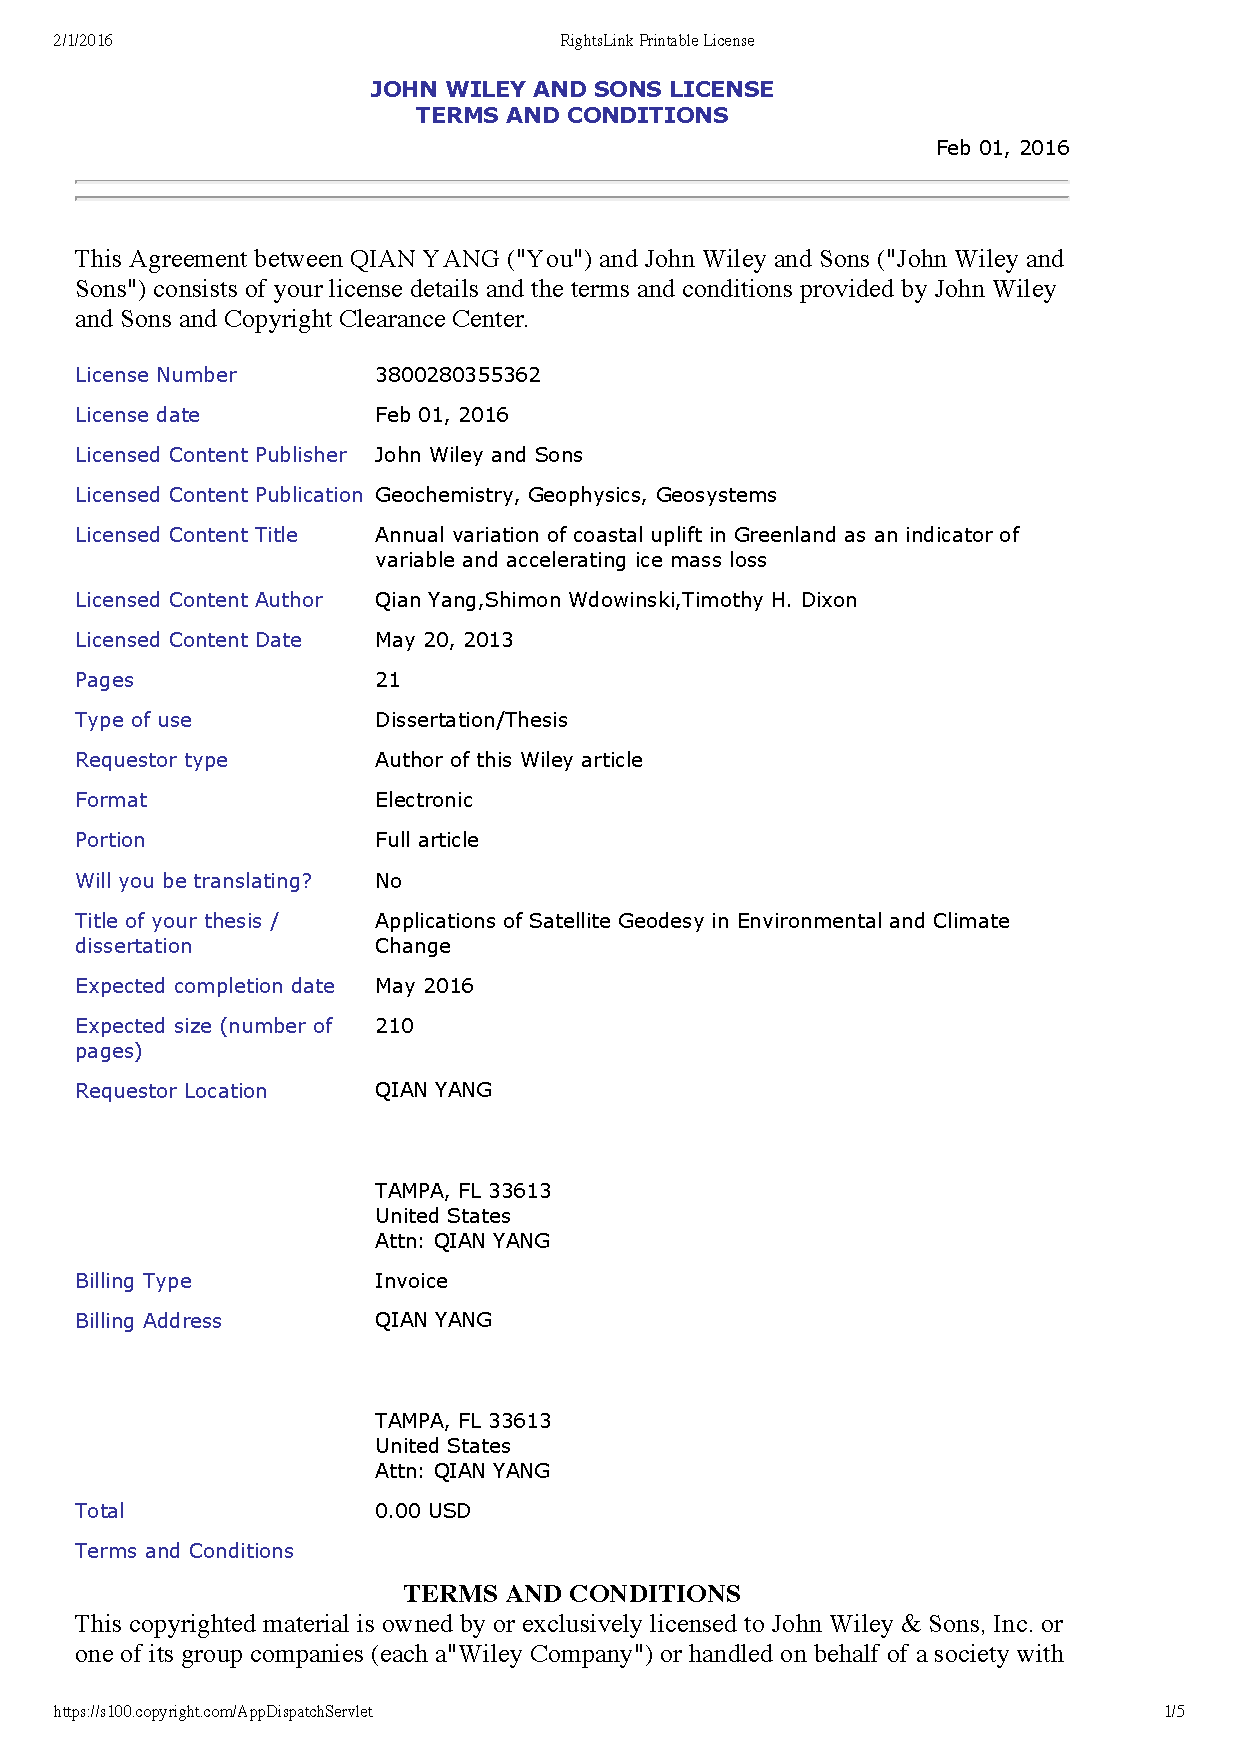
\includepdf[pages={1},scale=0.75,pagecommand={\section*{Appendix C: Copyright permission}\addcontentsline{toc}{section}{Appendix C: Copyright permission}}]{/Users/qianyang/Dropbox/Disseratation/dissertation_latex/copyright/chpt3.pdf}
\includepdf[pages={2-5},scale=0.75]{/Users/qianyang/Dropbox/Disseratation/dissertation_latex/copyright/chpt3.pdf}
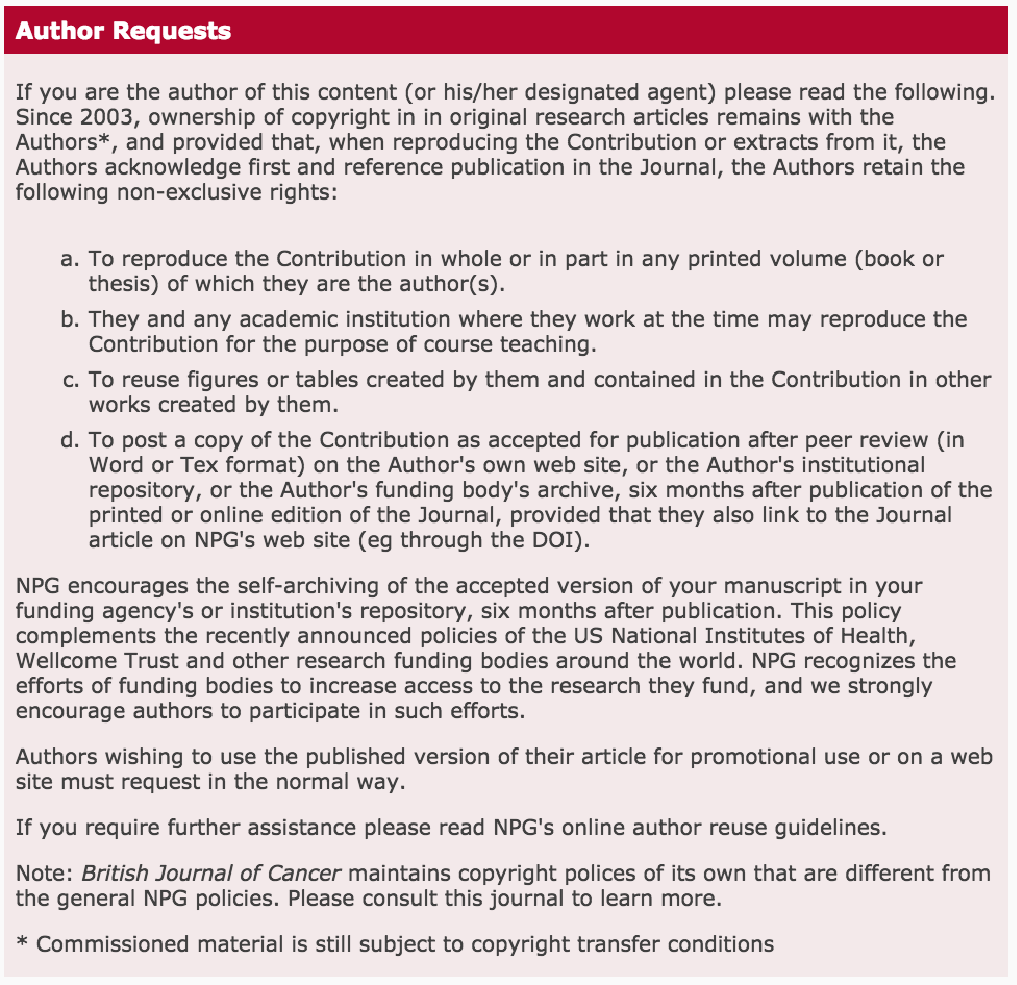
\includepdf[pages={1-},scale=0.75]{/Users/qianyang/Dropbox/Disseratation/dissertation_latex/copyright/chpt4.pdf}
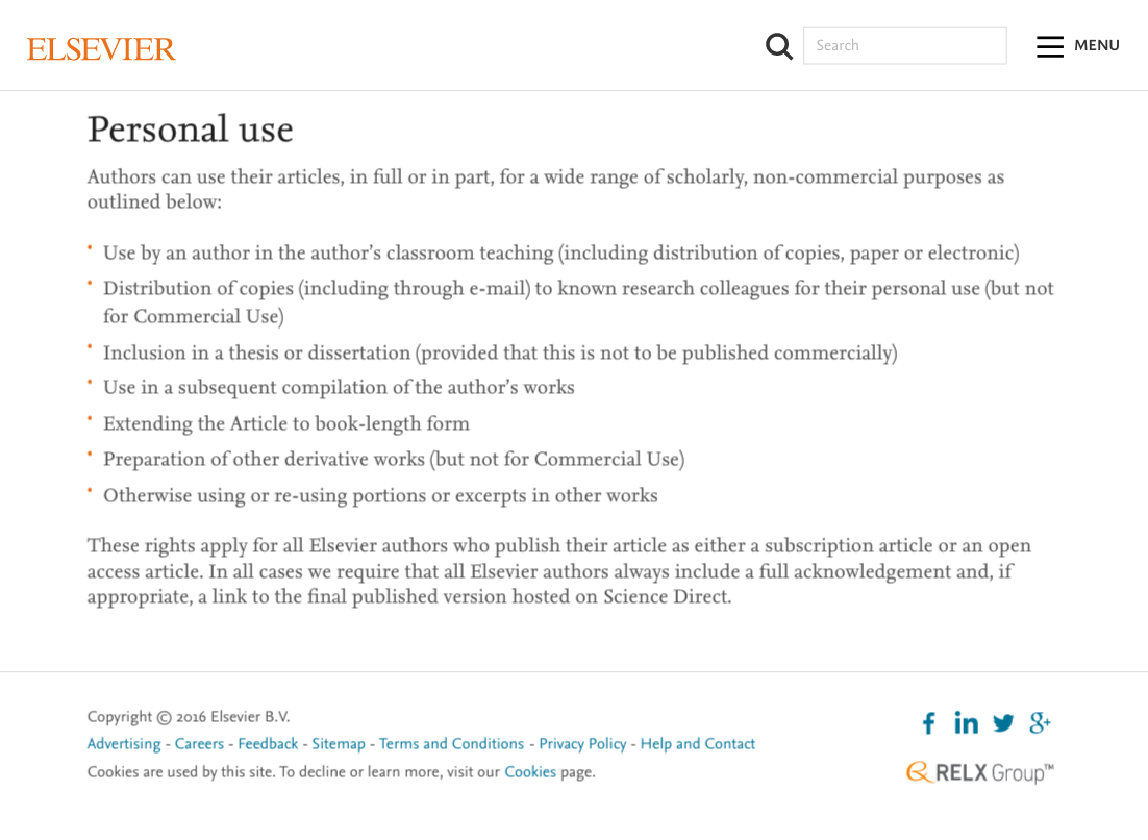
\includepdf[pages={1-},scale=0.75]{/Users/qianyang/Dropbox/Disseratation/dissertation_latex/copyright/chpt5.pdf}

\clearpage
\section*{Appendix D: References}
\addcontentsline{toc}{section}{Appendix D: References}
\bibliography{app_ref}
\bibliographystyle{apalike}

%insert tables for chapter 3
\clearpage
\begin{table}[h!]
	\centering
	\caption{Comparison of seasonal uplift patterns parameters estimated from fitting GPS vertical time series with and without atmospheric loading correction to a cubic spline model.}
	\begin{adjustbox}{width=1\textwidth}
	\begin{threeparttable}
		\begin{tabular}{lcccccc}
			\midrule
			&\multicolumn{2}{c}{2008} & \multicolumn{2}{c}{2009} & \multicolumn{2}{c}{2010} \\
			& No APLC & APLC & NO APLC & APLC & NO APLC & APLC \\
			\midrule
			Start time (doy) & N/D & N/D & 146 & 150 & 142 & 153\\
			End time (doy) & 320 & 315 & 323 & 321 & 327 & 332\\
			Duration (days) & N/D & N/D & 177 & 171 & 185 & 179\\
			Uplift (mm) & N/D & N/D & 9.2 & 11.5 & 16 & 19.3\\
			Uplift rate($10^{-2}$ mm day$^{-1}$) & N/D & N/D & 5.2 & 6.7 & 8.7 & 10.8\\
			\midrule
		\end{tabular}
		\begin{tablenotes}
			\small
			\item $\bullet$ NO ALC mean no atmospheric loading correction is applied; ALC means atmospheric loading correction is applied. 
			\item $\bullet$ Other symbols are the same as in Table \ref{tab:chpt3_table1}.
		\end{tablenotes}
		\end{threeparttable}
	\end{adjustbox}
	\label{tab:SI_chpt3_table1}
\end{table}

\clearpage
\begin{table}[h!]
\centering
\caption{List of meteorological stations}
\begin{adjustbox}{width=1\textwidth}
\begin{threeparttable}
\begin{tabular}{lccccccc}
	\midrule
	WMO-ID and & Latitude & Longitude & Elevation & Near GPS site & Horizontal dist & Elevation Diff & Distance \\
	station name & (deg N) & (deg E) & (m.a.s) & & (km) & (m) & (km)\\
	\midrule
	04205 Mitt.Qaanaaq* & 77.48 & -69.38 & 16 & DKSG & 231.4 & 579 & 231.4\\
	&  &  &  & MARG & 95.7 & 641 & 95.7\\
	&  &  &  & THU3 & 105.5 & 20 & 105.5\\
	04208 Kitsissorsuit & 74.03 & -57.82 & 40 & KULL & 63.4 & 54 & 63.4\\
	04211 Mitt.Upernavik & 72.78 & -56.13 & 126 & SRMP & 58.8 & 218 & 58.8\\
	04213 Mitt.Qaarsut & 70.73 & -52.70 & 88 & QAAR & 0.8 & 35 & 0.8\\
	&  &  &  & RINK & 138.4 & 1252 & 138.4\\
	04221 Mitt.Iiulissat & 69.23 & -51.07 & 29 & KAGA & 49.5 & 120 & 49.5\\
	04231 Kangerlussuaq* & 67.02 & -51.70 & 50 & KELY & 10.8 & 194 & 10.8\\
	04272 Qaqortoq* & 60.72 & -46.05 & 32 & SENU & 71.6 & 634 & 71.6\\
	&  &  &  & QAQ1 & 1.0 & 78 & 1.0\\
	04351 Aputiteeq & 67.78 & -32.30 & 13 & PLPK & 123.1 & 56 & 123.1\\
	04360 Tasiilaq* & 65.60 & -37.62 & 53 & HEL2 & 93.1 & 374 & 93.1\\
	&  &  &  & KULU & 21.5 & 14 & 21.5\\
	04361 Mitt.Kulusuk & 65.58 & -37.15 & 35 & KSNB & 158.6 & 1624 & 158.6\\
	04373 Ikermit & 64.78 & -40.30 & 85 & HJOR & 157.3 & 680 & 157.3\\
	&  &  &  & LYNS & 39.6 & 89 & 39.6\\
	&  &  &  & TREO & 76.2 & 38 & 76.2\\
	&  &  &  & TIMM & 268.3 & 230 & 268.3\\
	\midrule
\end{tabular}
\begin{tablenotes}
	\small
	\item $\bullet$ WMO-ID and station information are provided by Technical Report 11-10 of Danish Meteorological Institute.  
	\item $\bullet$ Horizontal dist: horizontal distance between GPS site and nearby MET station. 
	\item $\bullet$ Elevation diff: elevation difference between GPS site and nearby MET station.
\end{tablenotes}
\end{threeparttable}
\end{adjustbox}
\label{tab:SI_chpt3_table2}
\end{table}

\clearpage
\begin{center}
\begin{ThreePartTable}
\begin{longtable}{lccc}
\caption{Five parameters of seasonal uplift patterns estimated from fitting GPS vertical data to a cubic spline model and parameters describing both atmospheric and oceanic condition at each GPS site.}\\
\midrule 
\multicolumn{1}{c}{Year} & 2008 & 2009 & 2010 \\
\midrule 
\multicolumn{1}{c}{DKSG} & & & \\
				Start time (doy) & 136$\pm$12 & 233$\pm$7 & 197$\pm$5\\
				End time (doy) & 370$\pm$7 & 382$\pm$4 & 359$\pm$5\\
				Duration (days) & 234$\pm$12 & 149$\pm$7 & 162$\pm$6\\
				Uplift (mm) & 5.2$\pm$0.8 & 8.3$\pm$0.8 & 8.1$\pm$1.0\\
				Uplift rate ($10^{-2}$ mm day$^{-1}$) & 2.2$\pm$0.4 & 5.6$\pm$0.4 & 5.0$\pm$0.5\\
				AMSAT ($\textordmasculine$ C) & -9.2 & -9.0 & -6.8\\
				CAPDD (days) & 113 & 107 & 116\\
				AMSSWT ($\textordmasculine$ C) & 0.5 & 0.3 & 0.5\\
				&  &  & \\
				\multicolumn{1}{c}{HEL2} & & & \\
				Start time (doy) & 144$\pm$5 & 154$\pm$5 & 174$\pm$2\\
				End time (doy) & 348$\pm$3 & 350$\pm$3 & 361$\pm$2\\
				Duration (days) & 204$\pm$5 & 196$\pm$5 & 187$\pm$3\\
				Uplift (mm) & 12.2$\pm$0.7 & 9.0$\pm$0.7 & 19.0$\pm$0.8\\
				Uplift rate ($10^{-2}$ mm day$^{-1}$) & 6.0$\pm$0.4 & 4.6$\pm$0.3 & 10.2$\pm$0.4\\
				AMSAT ($\textordmasculine$ C) & -0.5 & -0.2 & 1.0\\
				CAPDD (days) & 180 & 183 & 188\\
				AMSSWT ($\textordmasculine$ C) & 5.0 & 4.7 & 5.3\\
				&  &  & \\
				\multicolumn{1}{c}{HJOR} & & & \\
				Start time (doy) & 133$\pm$8 & 174$\pm$7 & 155$\pm$3\\
				End time (doy) & 336$\pm$3 & 344$\pm$3 & 346$\pm$2\\
				Duration (days) & 224$\pm$8 & 169$\pm$6 & 190$\pm$3\\
				Uplift (mm) & 12.5$\pm$0.7 & 7.0$\pm$0.6 & 18.3$\pm$0.7\\
				Uplift rate ($10^{-2}$ mm day$^{-1}$) & 5.6$\pm$0.4 & 4.2$\pm$0.3 & 9.6$\pm$0.4\\
				AMSAT ($\textordmasculine$ C) & -1.4 & -1.0 & 0.5\\
				CAPDD (days) & 155 & 155 & 195\\
				AMSSWT ($\textordmasculine$ C) & 5.4 & 5.1 & 5.8\\	
				&  &  & \\
				\multicolumn{1}{c}{KAGA} & & & \\
				Start time (doy) & 149$\pm$8 & 186$\pm$4 & 158$\pm$3\\
				End time (doy) & 367$\pm$3 & 362$\pm$3 & 338$\pm$2\\
				Duration (days) & 218$\pm$8 & 177$\pm$4 & 180$\pm$3\\
				Uplift (mm) & 7.6$\pm$0.7 & 8.2$\pm$0.7 & 16.7$\pm$0.8\\
				Uplift rate ($10^{-2}$ mm day$^{-1}$) & 3.5$\pm$0.4 & 4.7$\pm$0.4 & 9.3$\pm$0.4\\
				AMSAT ($\textordmasculine$ C) & -3.7 & -3.2 & 0.0\\
				CAPDD (days) & 148 & 144 & 182\\
				AMSSWT ($\textordmasculine$ C) & 2.0 & 1.6 & 2.3\\
				&  &  & \\
				\multicolumn{1}{c}{KELY} & & & \\
				Start time (doy) & 153$\pm$28 & 205$\pm$74 & 108$\pm$36\\
				End time (doy) & 356$\pm$21 & 373$\pm$54 & 335$\pm$12\\
				Duration (days) & 203$\pm$29 & 169$\pm$75 & 228$\pm$35\\
				Uplift (mm) & 6.4$\pm$2.2 & 2.1$\pm$2.2 & 14.1$\pm$2.5\\
				Uplift rate ($10^{-2}$ mm day$^{-1}$) & 3.2$\pm$0.4 & 1.2$\pm$0.5 & 6.2$\pm$0.6\\
				AMSAT ($\textordmasculine$ C) & -4.4 & -4.7 & -0.2\\
				CAPDD (days) & 163 & 148 & 196\\
				AMSSWT ($\textordmasculine$ C) & 2.5 & 2.3 & 3.1\\
				&  &  & \\
				\multicolumn{1}{c}{KSNB} & & & \\
				Start time (doy) & 133$\pm$10 & 221$\pm$5 & 183$\pm$4\\
				End time (doy) & 370$\pm$5 & 366$\pm$3 & 375$\pm$4\\
				Duration (days) & 238$\pm$10 & 145$\pm$5 & 192$\pm$5\\
				Uplift (mm) & 9.6$\pm$0.8 & 7.6$\pm$0.6 & 12.0$\pm$0.8\\
				Uplift rate ($10^{-2}$ mm day$^{-1}$) & 4.1$\pm$0.4 & 5.2$\pm$0.4 & 6.3$\pm$0.4\\
				AMSAT ($\textordmasculine$ C) & -1.3 & -0.6 & 0.5\\
				CAPDD (days) & 153 & 170 & 192\\
				AMSSWT ($\textordmasculine$ C) & 5.0 & 4.8 & 5.4\\ 
				&  &  & \\
				\multicolumn{1}{c}{KULL} & & & \\
Start time (doy) & 247$\pm$9 & 250$\pm$4 & 208$\pm$5\\
End time (doy)&393$\pm$5&399$\pm$5&355$\pm$4\\
Duration (days)&146$\pm$8&149$\pm$5&147$\pm$5\\
Uplift (mm)&6.0$\pm$0.7&8.5$\pm$0.7&6.5$\pm$0.8\\
Uplit rate ($10^{-2}$ mm day$^{-1}$)&4.1$\pm$0.4&5.7$\pm$0.4&4.4$\pm$0.4\\
AMSAT ($\textordmasculine$C)&-7.4&-7.0&-4.7\\
CAPDD (days)&108&108&138\\
AMSSWT ($\textordmasculine$C)&1.0&0.7&1.0\\																				
				&  &  & \\	
\multicolumn{1}{c}{KULU} & & & \\
Start time (doy)&318$\pm$179&110$\pm$36&108$\pm$24\\
End time (doy)&116$\pm$204&312$\pm$22&334$\pm$10\\
Duration (days)&-179$\pm$380&207$\pm$36&227$\pm$24\\
Uplift (mm)&5.1$\pm$5.1&2.9$\pm$1.7&11.9$\pm$2.0\\
Uplit rate ($10^{-2}$ mm day$^{-1}$)&0.0$\pm$1.0&1.4$\pm$0.3&5.2$\pm$0.4\\
AMSAT ($\textordmasculine$C)&-0.5&-0.2&1.0\\
CAPDD (days)&180&183&188\\
AMSSWT ($\textordmasculine$C)&5.3&4.9&5.7\\
&  &  & \\	
\multicolumn{1}{c}{LYNS} & & & \\
Start time (doy)&121$\pm$8&259$\pm$4&210$\pm$6\\
End time (doy)&374$\pm$8&401$\pm$6&361$\pm$4\\
Duration (days)&254$\pm$11&142$\pm$5&151$\pm$6\\
Uplift (mm)&4.6$\pm$0.8&7.2$\pm$0.8&6.9$\pm$0.8\\
Uplit rate ($10^{-2}$ mm day$^{-1}$)&1.8$\pm$0.4&5.1$\pm$0.4&4.6$\pm$0.5\\
AMSAT ($\textordmasculine$C)&-9.2&-9.0&-6.8\\
CAPDD (days)&113&107&116\\
AMSSWT ($\textordmasculine$C)&0.3&0.1&0.2\\
&  &  & \\
\multicolumn{1}{c}{MARG} & & & \\
Start time (doy)&77$\pm$10&193$\pm$11&172$\pm$3\\
End time (doy)&355$\pm$4&369$\pm$3&356$\pm$2\\
Duration (days)&278$\pm$11&176$\pm$11&185$\pm$3\\
Uplift (mm)&11.1$\pm$0.7&7.2$\pm$0.6&14.7$\pm$0.7\\
Uplit rate ($10^{-2}$ mm day$^{-1}$)&4.0$\pm$0.3&4.1$\pm$0.4&7.9$\pm$0.4\\
AMSAT ($\textordmasculine$C)&-1.4&-1.0&0.5\\
CAPDD (days)&155&155&195\\
AMSSWT ($\textordmasculine$C)&5.5&5.2&5.9\\
&  &  & \\
\multicolumn{1}{c}{PLPK} & & & \\
Start time (doy)&85$\pm$9&186$\pm$17&172$\pm$4\\
End time (doy)&344$\pm$5&352$\pm$4&379$\pm$10\\
Duration (days)&258$\pm$10&165$\pm$16&207$\pm$10\\
Uplift (mm)&9.8$\pm$0.8&5.8$\pm$0.7&14.2$\pm$1.0\\
Uplit rate ($10^{-2}$ mm day$^{-1}$)&3.8$\pm$0.3&3.6$\pm$0.4&6.9$\pm$0.4\\
AMSAT ($\textordmasculine$C)&-3.3&-3.1&-2.6\\
CAPDD (days)&125&142&146\\
AMSSWT ($\textordmasculine$C)&5.0&4.8&5.4\\
&  &  & \\	
\multicolumn{1}{c}{QAQ1} & & & \\
Start time (doy)&165$\pm$37&225$\pm$23&165$\pm$11\\
End time (doy)&350$\pm$19&384$\pm$13&370$\pm$8\\
Duration (days)&185$\pm$36&159$\pm$21&204$\pm$12\\
Uplift (mm)&3.6$\pm$1.6&5.1$\pm$1.5&12.4$\pm$1.7\\
Uplit rate ($10^{-2}$ mm day$^{-1}$)&1.9$\pm$0.4&3.2$\pm$0.4&6.1$\pm$0.4\\
AMSAT ($\textordmasculine$C)&0.5&1.4&4.6\\
CAPDD (days)&219&194&272\\
AMSSWT ($\textordmasculine$C)&4.6&4.3&4.9\\
&  &  & \\
\multicolumn{1}{c}{RINK} & & & \\
Start time (doy)&168$\pm$12&237$\pm$6&184$\pm$5\\
End time (doy)&376$\pm$6&380$\pm$3&357$\pm$4\\
Duration (days)&208$\pm$11&143$\pm$6&173$\pm$5\\
Uplift (mm)&6.9$\pm$0.8&7.3$\pm$0.7&10.0$\pm$0.8\\
Uplit rate ($10^{-2}$ mm day$^{-1}$)&3.3$\pm$0.4&5.1$\pm$0.4&5.6$\pm$0.4\\
AMSAT ($\textordmasculine$C)&-4.0&-3.8&-0.6\\
CAPDD (days)&135&129&184\\
AMSSWT ($\textordmasculine$C)&1.7&1.3&1.8\\
&  &  & \\
\multicolumn{1}{c}{SENU} & & & \\
Start time (doy)&N/D&151$\pm$3&152$\pm$2\\
End time (doy)&313$\pm$3&322$\pm$4&331$\pm$2\\
Duration (days)&N/D&170$\pm$4&179$\pm$2\\
Uplift (mm)&N/D&11.5$\pm$0.6&19.3$\pm$0.7\\
Uplit rate ($10^{-2}$ mm day$^{-1}$)&N/D&6.7$\pm$0.3&10.8$\pm$0.4\\
AMSAT ($\textordmasculine$C)&0.5&1.4&4.6\\
CAPDD (days)&219&194&270\\
AMSSWT ($\textordmasculine$C)&4.6&4.3&4.9\\
&  &  & \\	
\multicolumn{1}{c}{SRMP} & & & \\
Start time (doy)&150$\pm$13&238$\pm$5&174$\pm$4\\
End time (doy)&373$\pm$5&376$\pm$3&350$\pm$3\\
Duration (days)&223$\pm$13&139$\pm$5&176$\pm$4\\
Uplift (mm)&6.9$\pm$0.8&7.7$\pm$0.7&11.6$\pm$0.8\\
Uplit rate ($10^{-2}$ mm day$^{-1}$)&3.1$\pm$0.4&5.6$\pm$0.4&6.6$\pm$0.4\\
AMSAT ($\textordmasculine$C)&-6.0&-5.5&-3.1\\
CAPDD (days)&118&114&150\\
AMSSWT ($\textordmasculine$C)&1.1&0.8&1.1\\
&  &  & \\		
\multicolumn{1}{c}{THU3} & & & \\
Start time (doy)&76$\pm$277&218$\pm$37&211$\pm$16\\
End time (doy)&367$\pm$29&398$\pm$23&350$\pm$11\\
Duration (days)&333$\pm$257&184$\pm$36&139$\pm$16\\
Uplift (mm)&3.5$\pm$3.4&5.6$\pm$2.0&5.7$\pm$1.9\\
Uplit rate ($10^{-2}$ mm day$^{-1}$)&1.2$\pm$0.3&3.1$\pm$0.4&4.1$\pm$0.5\\
AMSAT ($\textordmasculine$C)&-9.2&-9.0&-6.8\\
CAPDD (days)&113&107&116\\
AMSSWT ($\textordmasculine$C)&0.3&0.1&0.2\\
&  &  & \\
\multicolumn{1}{c}{TIMM} & & & \\
Start time (doy)&151$\pm$7&196$\pm$9&181$\pm$3\\
End time (doy)&352$\pm$3&374$\pm$3&360$\pm$3\\
Duration (days)&200$\pm$7&177$\pm$8&179$\pm$3\\
Uplift (mm)&10.4$\pm$0.7&8.4$\pm$0.7&13.7$\pm$0.7\\
Uplit rate ($10^{-2}$ mm day$^{-1}$)&5.2$\pm$0.4&4.7$\pm$0.4&7.7$\pm$0.4\\
AMSAT ($\textordmasculine$C)&-1.4&-1.0&0.5\\
CAPDD (days)&155&155&195\\
AMSSWT ($\textordmasculine$C)&5.4&5.1&5.8\\
&  &  & \\
\multicolumn{1}{c}{TREO} & & & \\
Start time (doy)&122$\pm$6&176$\pm$6&162$\pm$4\\
End time (doy)&349$\pm$3&343$\pm$4&367$\pm$3\\
Duration (days)&227$\pm$6&167$\pm$6&205$\pm$4\\
Uplift (mm)&14.7$\pm$0.7&5.4$\pm$0.6&17.6$\pm$0.8\\
Uplit rate ($10^{-2}$ mm day$^{-1}$)&6.5$\pm$0.4&3.3$\pm$0.4&8.6$\pm$0.4\\
AMSAT ($\textordmasculine$C)&-1.4&-1.0&0.5\\
CAPDD (days)&155&155&195\\
AMSSWT ($\textordmasculine$C)&5.5&5.2&5.9\\
\midrule	
%%%%%%%%%%%%%%%%%%%%%%%%%%%%%%%%%%%%	
\end{longtable}
	\begin{tablenotes}
		\small
		\item $\bullet$ Symbols are the same as in Table \ref{tab:chpt3_table1}.
	\end{tablenotes}
	\label{tab:SI_chpt3_table3}
\end{ThreePartTable}
\end{center}

%insert figures for chapter 3
\clearpage
\begin{figure}
	\centering
	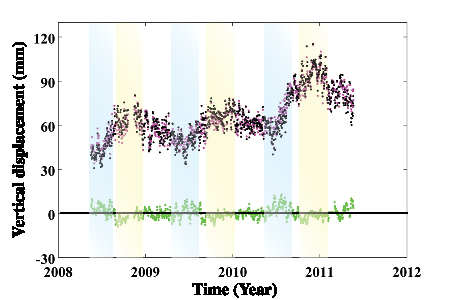
\includegraphics{figs_chpt3/2012GC004432-pA01.pdf}
	\caption[GPS time series from site SENU before (pink) and after (black) atmospheric pressure loading correction.]{GPS time series from site SENU before (pink) and after (black) atmospheric pressure loading correction. Green dots are vertical displacement due to atmospheric pressure loading. Light blue vertical bands mark approximate time period when atmospheric loading displacement is mainly positive. Light yellow vertical bands mark corresponding negative displacement.}
	\label{fig:SI3_fig1}
\end{figure}

\clearpage
\begin{figure}
	\centering
	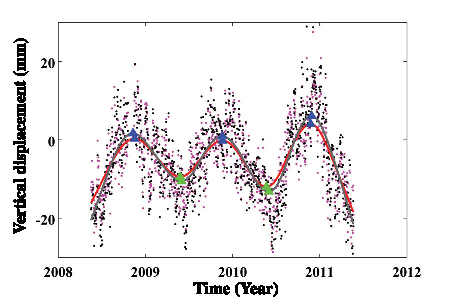
\includegraphics{figs_chpt3/2012GC004432-pA02.pdf}
	\caption[Example GPS time series for site SENU, de-trended and fit with annual model shown in Figure \ref{fig:fig2}.]{Example GPS time series for site SENU, de-trended and fit with annual model shown in \ref{fig:fig2}. Pink and black dots represent daily vertical position estimates before and after atmospheric pressure loading correction respectively. Red and grey curves are respective best-fit cubic splines with smoothing parameter set to 0.91.}
	\label{fig:SI3_fig2}
\end{figure}

\clearpage
\begin{figure}
	\centering
	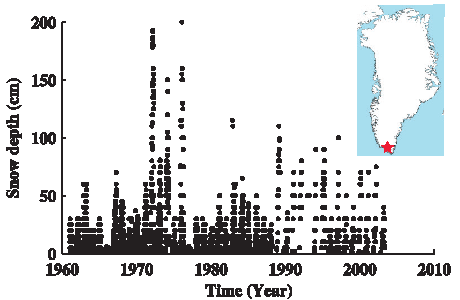
\includegraphics{figs_chpt3/2012GC004432-pA03.pdf}
	\caption[Snow depth recorded at a meteorological station  (WMO-ID 04272, Table \ref{tab:SI_chpt3_table2}) in southern Greenland coastal area.]{Snow depth recorded at a meteorological station  (WMO-ID 04272, Table \ref{tab:SI_chpt3_table2}) in southern Greenland coastal area.  Red star indicates location of the meteorological station.}
	\label{fig:SI3_fig3}
\end{figure}

\clearpage
\begin{figure}
	\centering
	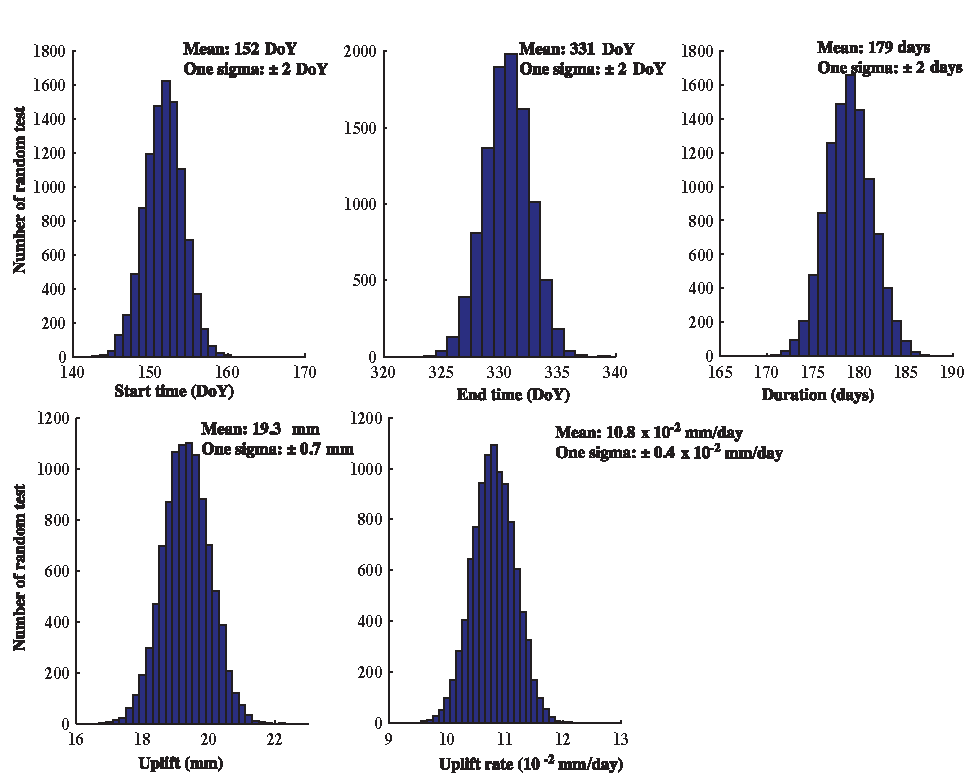
\includegraphics{figs_chpt3/2012GC004432-pA04.pdf}
	\caption[Histogram showing statistical result for five seasonal uplift variables at GPS station SENU.]{Histogram showing statistical result for five seasonal uplift variables at GPS station SENU.  Five variables are normally distributed.}
	\label{fig:SI3_fig4}
\end{figure}

\clearpage
\begin{figure}
	\centering
	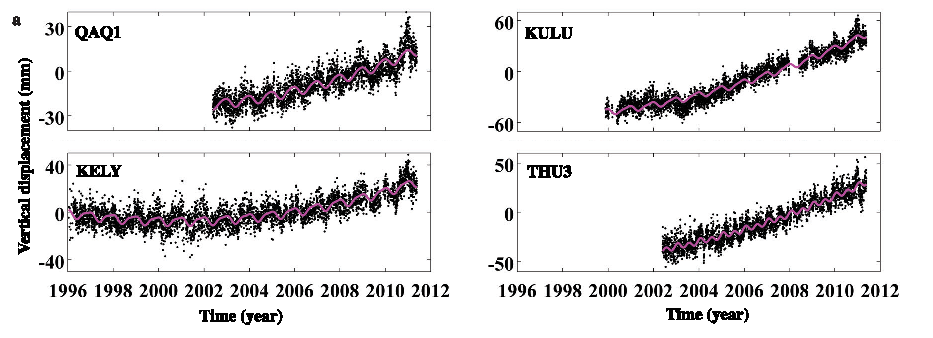
\includegraphics{figs_chpt3/2012GC004432-pA05a.pdf}
	\label{fig:SI3_fig5a}
\end{figure}

\clearpage
\begin{figure}
	\centering
	\includegraphics{figs_chpt3/2012GC004432-pA05b.pdf}
	\caption[Time series of GPS vertical component position.]{Time series of GPS vertical component position.  (a) Time series of long-term GPS records. (b) Time series of short-term GPS records.  For comparison with other sites, time series between mid-2007 and early 2011 at sites KULU, QAQ1, KELY and KULU are also shown in (b).  Vertical position is relative to arbitrary position. Pink curve shows constant acceleration model, including annual and semi-annual components.  GPS stations are organized from south to north.}
	\label{fig:SI3_fig5b}
\end{figure}

\clearpage
\begin{figure}
	\centering
	\includegraphics{figs_chpt3/2012GC004432-pA06a.pdf}
	\label{fig:SI3_fig6a}
\end{figure}

\clearpage
\begin{figure}
	\centering
	\includegraphics{figs_chpt3/2012GC004432-pA06b.pdf}
	\caption[Time series of GPS vertical component position after removing long-term trend by low pass filter.]{Time series of GPS vertical component position after removing long-term trend by low pass filter. (a) Time series of long-term GPS records. (b) Time series of short-term GPS records. In (b), we zoom in to the last 3 years of four long time series. Red curve is cubic spline best-fit model with 0.91 as smoothing parameter.  Blue triangle is the maximum value per year, and green triangle is the minimum value per year.}
	\label{fig:SI3_fig6b}
\end{figure}

\clearpage
\begin{figure}
	\centering
	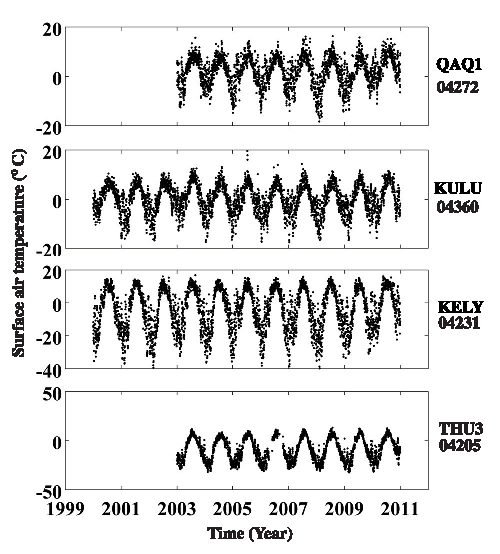
\includegraphics{figs_chpt3/2012GC004432-pA07.pdf}
	\caption[Time series of surface air temperature at meteorological stations near 4 GPS site.]{Time series of surface air temperature at meteorological stations near 4 GPS site.  Name of nearby GPS site and WMO-ID are on the right side of each plot. }
	\label{fig:SI3_fig7}
\end{figure}

%insert figures for chapter 4
\clearpage
\begin{figure}
\centering
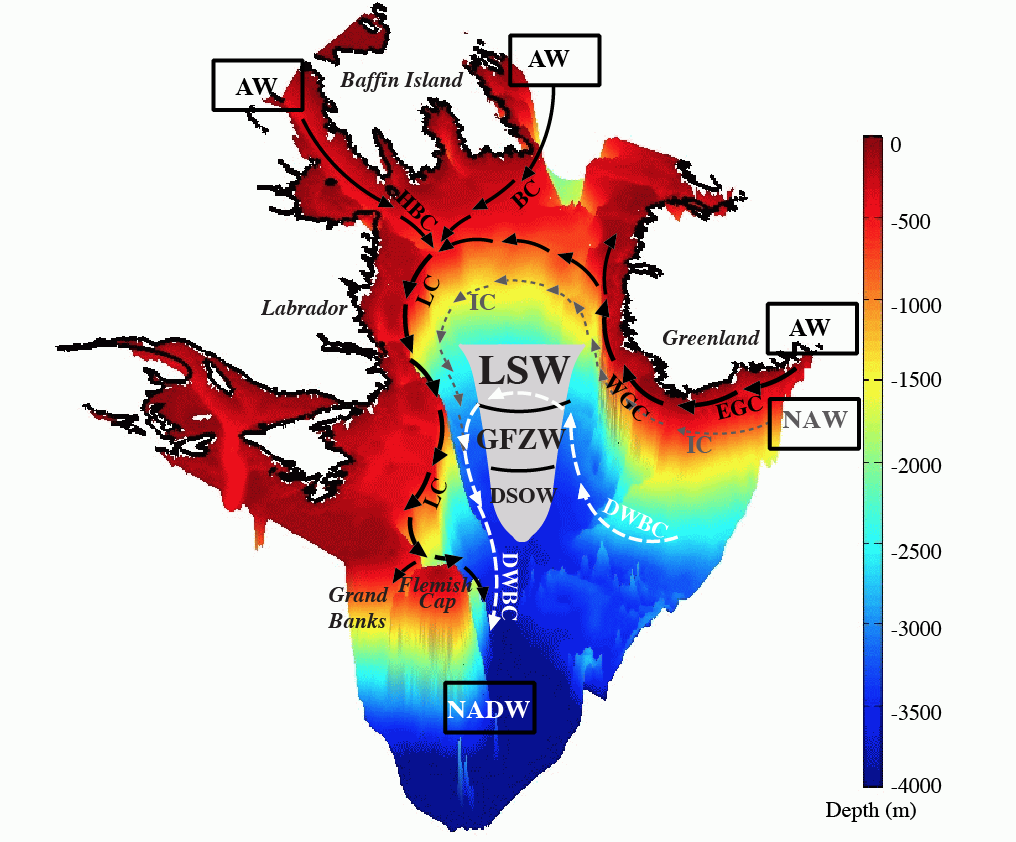
\includegraphics{figs_app/FigS1.png}
\caption[Simplified sketch illustrating 3-D structure of the Labrador Sea and major currents and water masses.]{Simplified sketch illustrating 3-D structure of the Labrador Sea and major currents and water masses. Black boxes represent water masses input to and output from the Labrador Sea along specific currents.  Arrows represent ocean currents at different depths: black solid arrows represent surface ocean currents carrying cold and fresh Arctic Water; grey dashed arrows represent subsurface ocean current carrying warm and salty North Atlantic Water; white dashed arrows represent the Deep Western Boundary Current that moves North Atlantic Deep Water southward.  EGC is East Greenland Current, WGC is West Greenland Current, HBC is Hudson's Bay Current, BC is Baffin Current, LC is Labrador Current, IC is Irminger Current, DWBC is Deep Western Boundary Current. AW is Arctic Water, NAW is North Atlantic Water, LSW is Labrador Sea Water, GFZW is Gibbs Fracture Zone Water, DSOW is Denmark Strait Overflow Water, NADW is North Atlantic Deep Water.  Not shown are the geographic sources of Arctic Water, which include the Greenland ice sheet, Arctic Ocean, Canadian Arctic Archipelago, and Hudson Bay, or the types of ice and water masses that contribute, which include glaciers and ice sheets, rivers, sea ice, and precipitation.  Also not shown are the major time scales for significant variability, which include annual (summer ice melting, winter cooling and convection) and decadal to multi-decadal (e.g., North Atlantic Oscillation, Atlantic Multi-decadal Oscillation).}
\label{fig:SI4_fig1}
\end{figure}

\begin{figure}
	\centering
	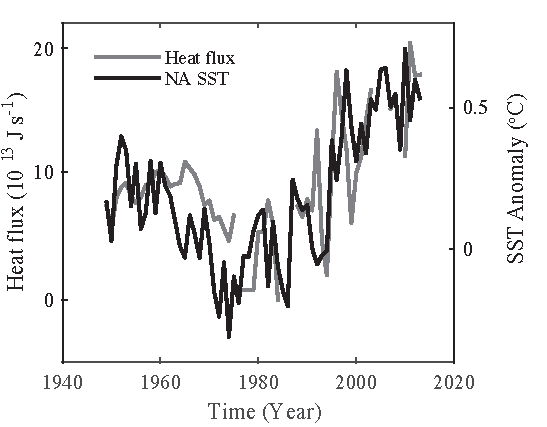
\includegraphics{figs_app/FigS2.pdf}
	\caption[Comparison of Irminger Water heat flux and North Atlantic SST anomaly over the period 1949 – 2013]{Comparison of Irminger Water heat flux and North Atlantic SST anomaly over the period 1949 – 2013.  Grey line indicates Irminger Water heat flux, black line indicates North Atlantic SST anomaly.  We use the HADISST dataset to compute SST anomaly.  We compute the annual average SST anomaly over a broad area of the North Atlantic, using as boundaries 0 $\textordmasculine$ - 60 $\textordmasculine$ North latitude and 0 $\textordmasculine$ - 80 $\textordmasculine$ West longitude, relative to the average temperature for the period 1901 to 1970.  Average North Atlantic SST anomaly shows a strong ($R=0.68$) and significant ($P=0.001$) correlation with our Irminger heat flux data for the 1949 to 2013 period, with both indices increasing strongly after 1995.}
	\label{fig:SI4_fig2}
\end{figure}

\begin{figure}
	\centering
	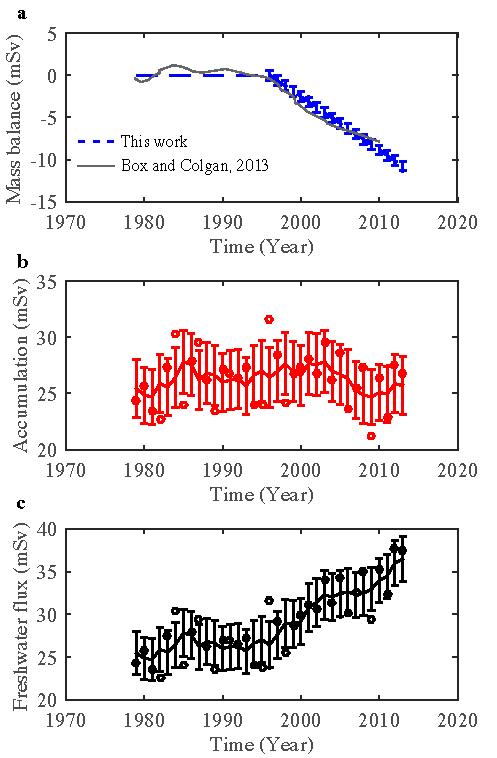
\includegraphics{figs_app/FigS3.pdf}
	\caption[Freshwater flux from Greenland estimated from mass balance and accumulation.  (a) Greenland mass balance.]{Freshwater flux from Greenland estimated from mass balance and accumulation.  (a) Greenland mass balance. Estimate from this study (blue dashed line) is compared with estimate from \citet{box2013greenland}. Blue error bars indicate uncertainty of mass balance, estimated at 95\% confidence level. (b) Greenland accumulation.  Red circles represent annual value.  Red solid line represents 5-year running average.  Red error bars indicate uncertainty of smoothed accumulation, which is approximated by uncertainty of accumulation modeled by RACMO2.3 ($\pm$ 9\%).  (c) Freshwater flux from Greenland.  Black circles represent freshwater flux from mass balance and annual accumulation (see equation \ref{eq:SI_chpt4_1}).  Black solid line represents freshwater flux from mass balance and smoothed accumulation.  Black error bars indicate propagated uncertainty.}
	\label{fig:SI4_fig3}
\end{figure}

\begin{figure}
	\centering
	\includegraphics{figs_app/FigS4.pdf}
	\caption[Comparison between estimates of freshwater flux from Greenland.]{Comparison between estimates of freshwater flux from Greenland.  (a) Comparison between two estimates of solid ice discharge from Greenland.  Blue line from \citet{bamber2012recent}, red line from \citet{enderlin2014improved}.  The estimate from \citet{bamber2012recent} required extrapolation to cover all Greenland discharge and is $\sim$3 mSv ($\sim$100 km 3 yr$^{-1}$) larger than the more recent estimate from \citet{enderlin2014improved}. (b) Comparison of three estimates of freshwater flux from Greenland: black line (this study), blue line (\citet{bamber2012recent}), red line (\citet{bamber2012recent}) with correction following \citet{enderlin2014improved}.}
	\label{fig:SI4_fig4}
\end{figure}

\begin{figure}
	\centering
	\includegraphics{figs_app/FigS5.pdf}
	\caption[Three estimates of the annual minimum Arctic sea ice volume time series.]{Three estimates of the annual minimum Arctic sea ice volume time series.  Red line represents estimate based on ice extent assuming 2 m thickness.  Blue line represents estimate based on ice area assuming 2 m thickness. Black line represents volume modeled by the Pan-Arctic Ice Ocean Modeling and Assimilation System (PIOMAS)\cite[]{zhang2003modeling}.  Error bars represent the uncertainty of annual minimum Arctic sea ice volume (1500 km$^{3}$).  (a) Three time series described above are fit with a two-slope model (thick solid line) (Supplementary methods).  Arrow marks the onset time of accelerated melting derived from three data sets: 1996 for ice extent and ice area data sets, 1997 for PIOMAS data set. (b) Three time series are fit with the linear state space model (thick solid line) (see methods in Appendix A). }
	\label{fig:SI4_fig5}
\end{figure}

\begin{figure}
	\centering
	\includegraphics{figs_app/FigS6.pdf}
	\caption[Long term melting rate of Arctic sea ice from three data sets.]{Long term melting rate of Arctic sea ice from three data sets.  Red line represents estimate based on ice extent data set.  Blue line represents estimate based on ice area data set. Black line represents estimate from the Pan-Arctic Ice Ocean Modeling and Assimilation System (PIOMAS) data set. The melting rate is estimated using the linear state space model (Figure \ref{fig:SI4_fig5}b).  Error bars indicate uncertainty at 95\% confidence level.}
	\label{fig:SI4_fig6}
\end{figure}

\begin{figure}
	\centering
	\includegraphics{figs_app/FigS7.pdf}
	\caption[Similar to Figure \ref{fig:chpt4_fig5} except salt flux of Irminger Water is expressed in terms of freshwater flux.]{Similar to Figure \ref{fig:chpt4_fig5} except salt flux of Irminger Water is expressed in terms of freshwater flux.  Grey solid line represents thickness of Labrador Sea Water.  Black solid line represents Arctic freshwater flux (the sum of freshwater flux from Greenland, the Canadian Arctic Archipelago and Arctic sea ice).  Dotted line represents freshwater flux of Irminger Water (IW). Salt flux is converted to freshwater flux using 34.80 as a reference salinity.}
	\label{fig:SI4_fig7}
\end{figure}

\begin{figure}
	\centering
	\includegraphics{figs_app/FigS8.pdf}
	\caption[Similar to Figure \ref{fig:chpt4_fig5} except grey solid line represents the mass of Labrador Sea Water.]{Similar to Figure \ref{fig:chpt4_fig5} except grey solid line represents the mass of Labrador Sea Water.  Black solid line represents Arctic freshwater flux (the sum of freshwater flux from Greenland, the Canadian Arctic Archipelago and Arctic sea ice). Density of Labrador Sea Water is obtained from the objective analyses of EN4.0.2 dataset from the UK Met Office Hadley Center\cite[]{good2013en4}.  Mass values are calculated by integrating density with volume between 50 $\textordmasculine$ N – 65 $\textordmasculine$ N, 38 $\textordmasculine$ W – 65 $\textordmasculine$ W and three depth range (900 – 2400 m, 1000 - 2500 m and 1100 – 2600 m), relative to the mean of 1950 – 2006. }
	\label{fig:SI4_fig8}
\end{figure}

\begin{figure}
	\centering
	\includegraphics{figs_app/FigS9a.pdf}
\end{figure}

\begin{figure}
	\centering
	\includegraphics{figs_app/FigS9b.pdf}
	\caption[Seasonal variation of freshwater flux from Greenland and the Canadian Arctic Archipelago.]{Seasonal variation of freshwater flux from Greenland and the Canadian Arctic Archipelago. (a) Monthly freshwater flux from Greenland (GL), Canadian Arctic Archipelago (CAA) and their total for 1979 – 2013.   Freshwater flux from Greenland and CAA peaks in July.  Freshwater flux since 2002 has exceeded 100 mSv for about a month a year 9 times, with 2012 having the highest value (150 mSv).  (b) Total summer (June, July and August) freshwater flux (solid line) compared to long-term averaged annual freshwater flux (dashed line).  Note that summer freshwater flux increased significantly about the time when GRACE data and a simple model of constant acceleration suggest that the current phase of accelerated Greenland mass loss began (red arrow) (see Figure \ref{fig:chpt4_fig2}).}
	\label{fig:SI4_fig9}
\end{figure}

\begin{figure}
	\centering
	\includegraphics{figs_app/FigS10.pdf}
	\caption[Predefined regions used in this paper to localize the GRACE mass change signal.]{Predefined regions used in this paper to localize the GRACE mass change signal.  Greenland is outlined with solid red line.}
	\label{fig:SI4_fig10}
\end{figure}

\begin{figure}
	\centering
	\includegraphics{figs_app/FigS11.pdf}
	\caption[Freshwater flux from Greenland and its two components.]{Freshwater flux from Greenland and its two components.  Black circles and solid line represent freshwater flux from Greenland.  Red circles and solid line represent freshwater flux component from ice mass loss.  Blue circles and solid line represent freshwater flux component from tundra runoff.  Circles represent annual value and solid line represents 5-year running average.  Black error bars indicate propagated uncertainty (Figure \ref{fig:SI4_fig3}).}
	\label{fig:SI4_fig11}
\end{figure}

\begin{figure}
	\centering
	\includegraphics{figs_app/FigS12.pdf}
	\caption[Freshwater flux from the Canadian Arctic Archipelago and its two components.]{Freshwater flux from the Canadian Arctic Archipelago and its two components.  Black circles and solid line represent freshwater flux from the Canadian Arctic Archipelago (CAA).  Red circles and solid line represent freshwater flux component from ice mass loss.  Blue circles and solid line represent freshwater flux component from tundra runoff.  Circle represents annual value and solid line represents 5-year running average.  Black error bars indicate uncertainty of smoothed freshwater flux from CAA, approximated by uncertainty of runoff modeled by RACMO2.3, believed to be accurate to $\pm$ 30\%\cite[]{lenaerts2013irreversible}.}
	\label{fig:SI4_fig12}
\end{figure}

\end{document}